\documentclass[a4paper,11pt, uplatex]{ujreport} % A4,11pt標準 for uplatex
\usepackage[top=30truemm,bottom=30truemm,left=30truemm,right=30truemm]{geometry}

\usepackage[dvipdfmx]{graphicx}
\usepackage[dvipdfmx, colorlinks=true, linkcolor=blue, citecolor=red, filecolor=black, urlcolor=blue]{hyperref}
\usepackage{amsmath,amssymb}
\usepackage{cleveref}
\usepackage{threeparttable}
\usepackage{enumerate}


%% subcaptionを使うためのもの
\makeatletter
\let\MYcaption\@makecaption
\makeatother

\usepackage{subcaption}
%\captionsetup{compatibility=false}      % 必要に応じて

\makeatletter
\let\@makecaption\MYcaption
\makeatother


\usepackage[left]{lineno}
%\pagewiselinenumbers
%% 行間を2倍
%\renewcommand{\baselinestretch}{2}
%\doublespacing

% コマンド類
\newcommand{\fknee}{$f_{{\rm knee}}$}
\newcommand{\he}{$^3{\rm He}$}
\newcommand{\Pint}{$P_{{\rm int}}$}
\newcommand{\Pread}{$P_{{\rm read}}$}
\newcommand{\ctext}[1]{\raise0.2ex\hbox{\textcircled{\scriptsize{#1}}}}

\renewcommand{\bibname}{参考文献}
\renewcommand{\baselinestretch}{1.1}


\begin{document}

% 表紙
\thispagestyle{empty}
\begin{center}
\vspace*{1cm}
{\LARGE {\bf {\rm 修士論文} } }\\
\vspace*{1.5cm}
\setlength{\baselineskip}{1cm}
%{\LARGE {\bf {\rm CMB観測実験に用いる超伝導検出器~MKID~のノイズ低減を行うための評価環境開発研究}}}\\
%{\LARGE {\bf {\rm CMB観測実験で用いる超伝導検出器MKIDの評価研究}}}\\
{\Large {\bf {\rm CMB観測実験GroundBIRDの焦点面検出器アライメントと\\
長期運用に向けた角度データ取得システムの最適化
% CMB観測におけるベースラインゆらぎの抑制研究
}}}\\
%{\LARGE {\bf {\rm CMB偏光観測実験GroundBIRDで用いる\\高透過率真空窓の開発研究}}}\\
\vspace{1.5cm}
{\Large 京都大学 理学研究科 物理学・宇宙物理学専攻}\\
%\vspace{0.01cm}
{\Large 物理学第二教室 高エネルギー物理学研究室}\\
\vspace{1.5cm}
{\Large 片岡~敬涼}\\
%\vspace{0.5cm}
\vspace{0.5cm}
{\Large 2025年1月 24日}
\begin{figure}[h]
 \centering
 
\includegraphics[width=0.6\columnwidth]{0_title/E-C.png}
\end{figure}


%\vspace{3cm}
%{\Large 2019年1月2日}

\end{center}

%

% abstract
\newpage
\begin{abstract}
\hspace{-4mm}

%gaiyou(CMBで迫りたい物理(ニュートリノ質量和、tau)、GB、自分のやったことがどう重要なのかを簡潔に記す)
宇宙マイクロ波背景放射(CMB)の温度異方性の観測によって、宇宙の進化を記述する標準理論が構築されてきた。現在ではCMBの偏光観測が大きなテーマとなっており、偏光を通してインフレーション理論やニュートリノ質量和、宇宙の再電離といった課題に迫ることができる。

GroundBIRDはスペイン領テネリフェ島の標高2,400 mに位置する大角度スケールの観測に特化した地上CMB望遠鏡である。望遠鏡を1分間で20回転させる高速スキャンによって大気揺らぎの影響を抑制した観測を行う。高速スキャンがもたらす効果を最大限に発揮するために、時間応答性の良い超伝導検出器MKIDを焦点面検出器として採用し、2023年5月から本格的な観測を開始した。大角度スケールでの偏光Eモードを観測することで、宇宙再電離期を特徴付け、さらにニュートリノ質量和と縮退したパラメータである光学的厚み$\tau$を誤差$\sigma_{\tau}\sim 0.01$で測定することを目指している。

観測を続けてデータを蓄積する段階にある現在、安定して長期運用をすること、そして質の良いデータを取得することが要求される。しかし、本研究の開始前の観測システムにおいて2つの未解決課題があった。1つは望遠鏡仰角データ取得システムが硬直的であること、もう1つは天球上での検出器配置がスキャン軸から傾いていることである。本論文ではこれらの課題に対する改善と最適化を行なった。

仰角データの取得にFPGAボードを使用しているが、人手を必要とするメンテナンスを高頻度で要し、システム運用をリモート主体で行えないことが、長期運用に対する障壁となっていた。本論文ではボード内のFPGAチップにPYNQと呼ばれるOSシステムを搭載し、OS上からソフトウェアを動かすことでデータ取得の操作性向上とアクセス性の向上を図ることにした。本研究でこのシステムを開発し、望遠鏡にインストールし、信号処理の確認と安定動作を確認した。

焦点面に搭載した多数のMKIDによってCMBの偏光信号を検出する。ここで、無偏光な大気放射ノイズを抑制するためにスキャン軸上の異なるMKID間で信号の差分をとる。しかし、スキャン軸とMKIDの配置軸に傾きがあると差分をとっても大気放射ノイズを十分に差し引けない。本研究では、月の観測データからこの問題を定量的に洗い出した。具体的には、MKIDの配置軸が望遠鏡のスキャン軸に対して約6°傾いていることを見積もった。そして、この結果をもとに、焦点面を含む望遠鏡の構造体を回転させることで天球上でのMKIDの配置軸を改善した。本研究ではさらに月と木星の観測データからこの改善の確認も行なった。加えて、スキャン軸上に配置されているMKID間で信号差分をとり、各入射信号の相関の強さを示す指標に焼き直し、回転の前後で比較することで観測する大気の揺らぎを抑制する結果を得た。

以上2点の改善と最適化を通してGroundBIRDが持つ運用、観測性能の向上を成功させた。



%本論文の構成を述べる。第\ref{chapter1}章でCMBに関わる理論的な背景、第\ref{chapter2}章でGroundBIRD実験の概要を説明する。以降は第\ref{chapter3}章と第\ref{chapter4}章の2部構成になっており、第\ref{chapter3}章でGroundBIRDの角度データ取得システムの改善について、第\ref{chapter4}章で焦点面検出器のアライメント較正とその結果について述べる。第\ref{chapter5}章で今後の展望を述べ、第\ref{chapter6}章でまとめを述べる。


\end{abstract}


%\thispagestyle{empty}
%

% 目次
\newpage
\pagenumbering{roman}
\setcounter{page}{1}
\setcounter{tocdepth}{2}
\tableofcontents
%\listoffigures
%


% 本文
\newpage
\pagestyle{headings}
\pagenumbering{arabic}
\setcounter{page}{1}
\setlength\floatsep{0pt} %dblfloatsep		%ページの上下に出力される図と図の間のスペース
\setlength\abovecaptionskip{0pt}	%図とキャプションの間のスペース


%
\include{2_cosmology/kk_Introduction}
\chapter{GroundBIRD実験}
\label{chapter2}

CMB観測実験には地上から観測する実験と衛星を用いて宇宙から観測する実験に分けられる。ここでは私が参加しているGroundBIRD実験(図\ref{GB_overview})について実験の概要と現在の観測状況について説明する。

\begin{figure}[htbp]
  \centering
  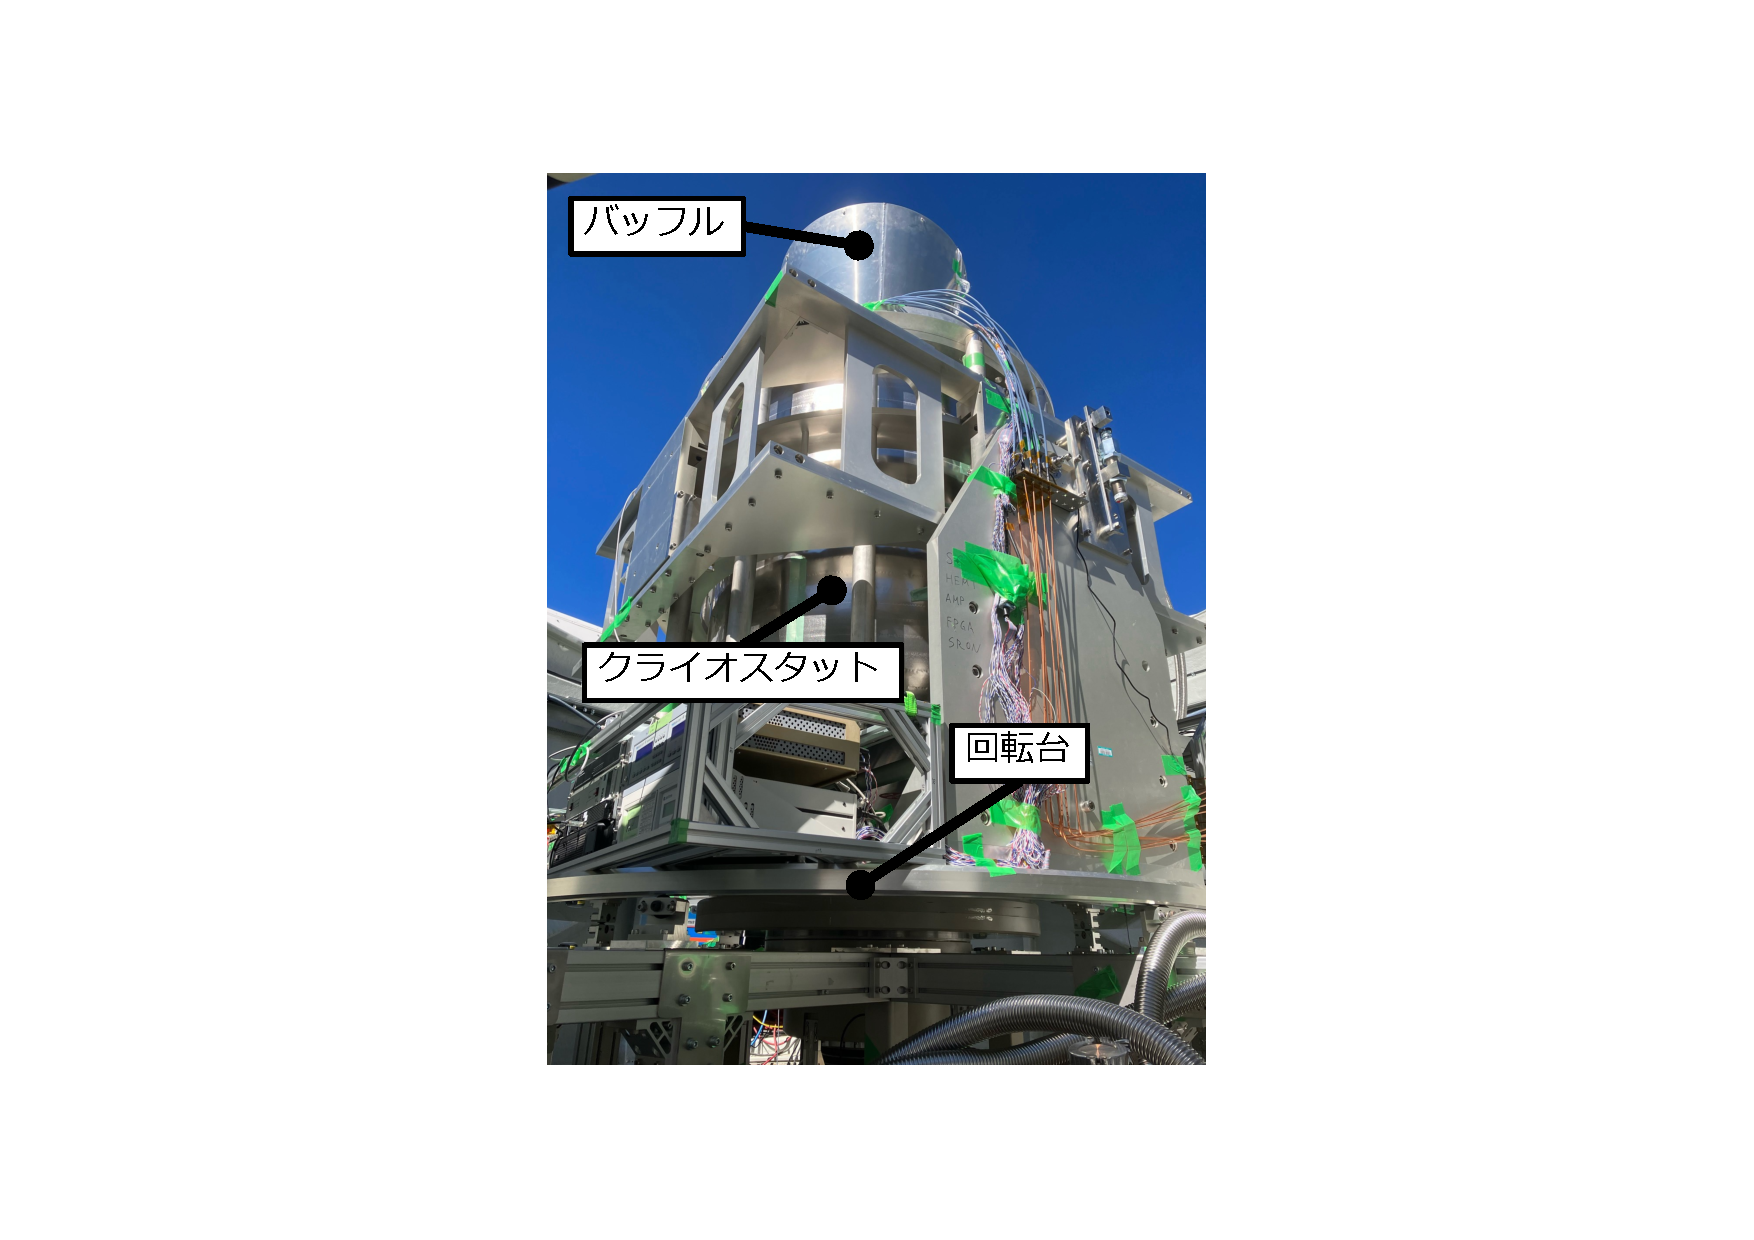
\includegraphics[width=0.5\columnwidth]{3_GB/figs/GB_overview2.pdf}
  \caption{GroundBIRD望遠鏡の外観。望遠鏡クライオスタットが方位角回転台の上に設置されており、回転台とともに最大で20RPM(1分間で20回転)の速度で回転する。}
  \label{GB_overview}
\end{figure}
\section{実験概要}

\subsection{GroundBIRD望遠鏡とスキャン戦略}
GroundBIRD望遠鏡はスペイン領カナリア諸島の1つであるテネリフェ島のテイデ観測所(高度2,400m)に位置する地上CMB望遠鏡である。地上からの観測において最も邪魔なのが大気からの放射であるが、テイデ観測所は大気中の積算水蒸気量(Precipitable Water Vapor、以下PWVと略す)がおよそ3.5mm\cite{PWV}と、観測に適した場所である。

GroundBIRDはスキャン戦略に大きな特徴を持つ。地上からの観測では大気放射に由来するノイズが本来見たいCMBに混入する。大気放射は無偏光であるが、観測装置の不完全性などで誤って偽偏光として観測されるおそれがある。特に、大気は刻一刻と揺らいでいるため、観測する空の領域ごとで観測される大気のノイズも揺らぎ、偽偏光を検出する影響は無視できなくなる。その影響を回避するためには大気揺らぎを抑制する変調が必要になる。GroundBIRDでは、望遠鏡を最大で20RPM(3秒で1回転)させる独自のスキャン戦略をとることで大気揺らぎを抑制したCMB観測を実現する。加えて望遠鏡の仰角を$70^{\circ}$に固定し、方位角方向に高速スキャンさせることで、全天の広い領域を観測することができる。望遠鏡の連続回転と地球の自転を組み合わせることで全天の約45$\%$を観測することができる(図\ref{scan_strategy})。

\begin{figure}[htbp]
  \centering
  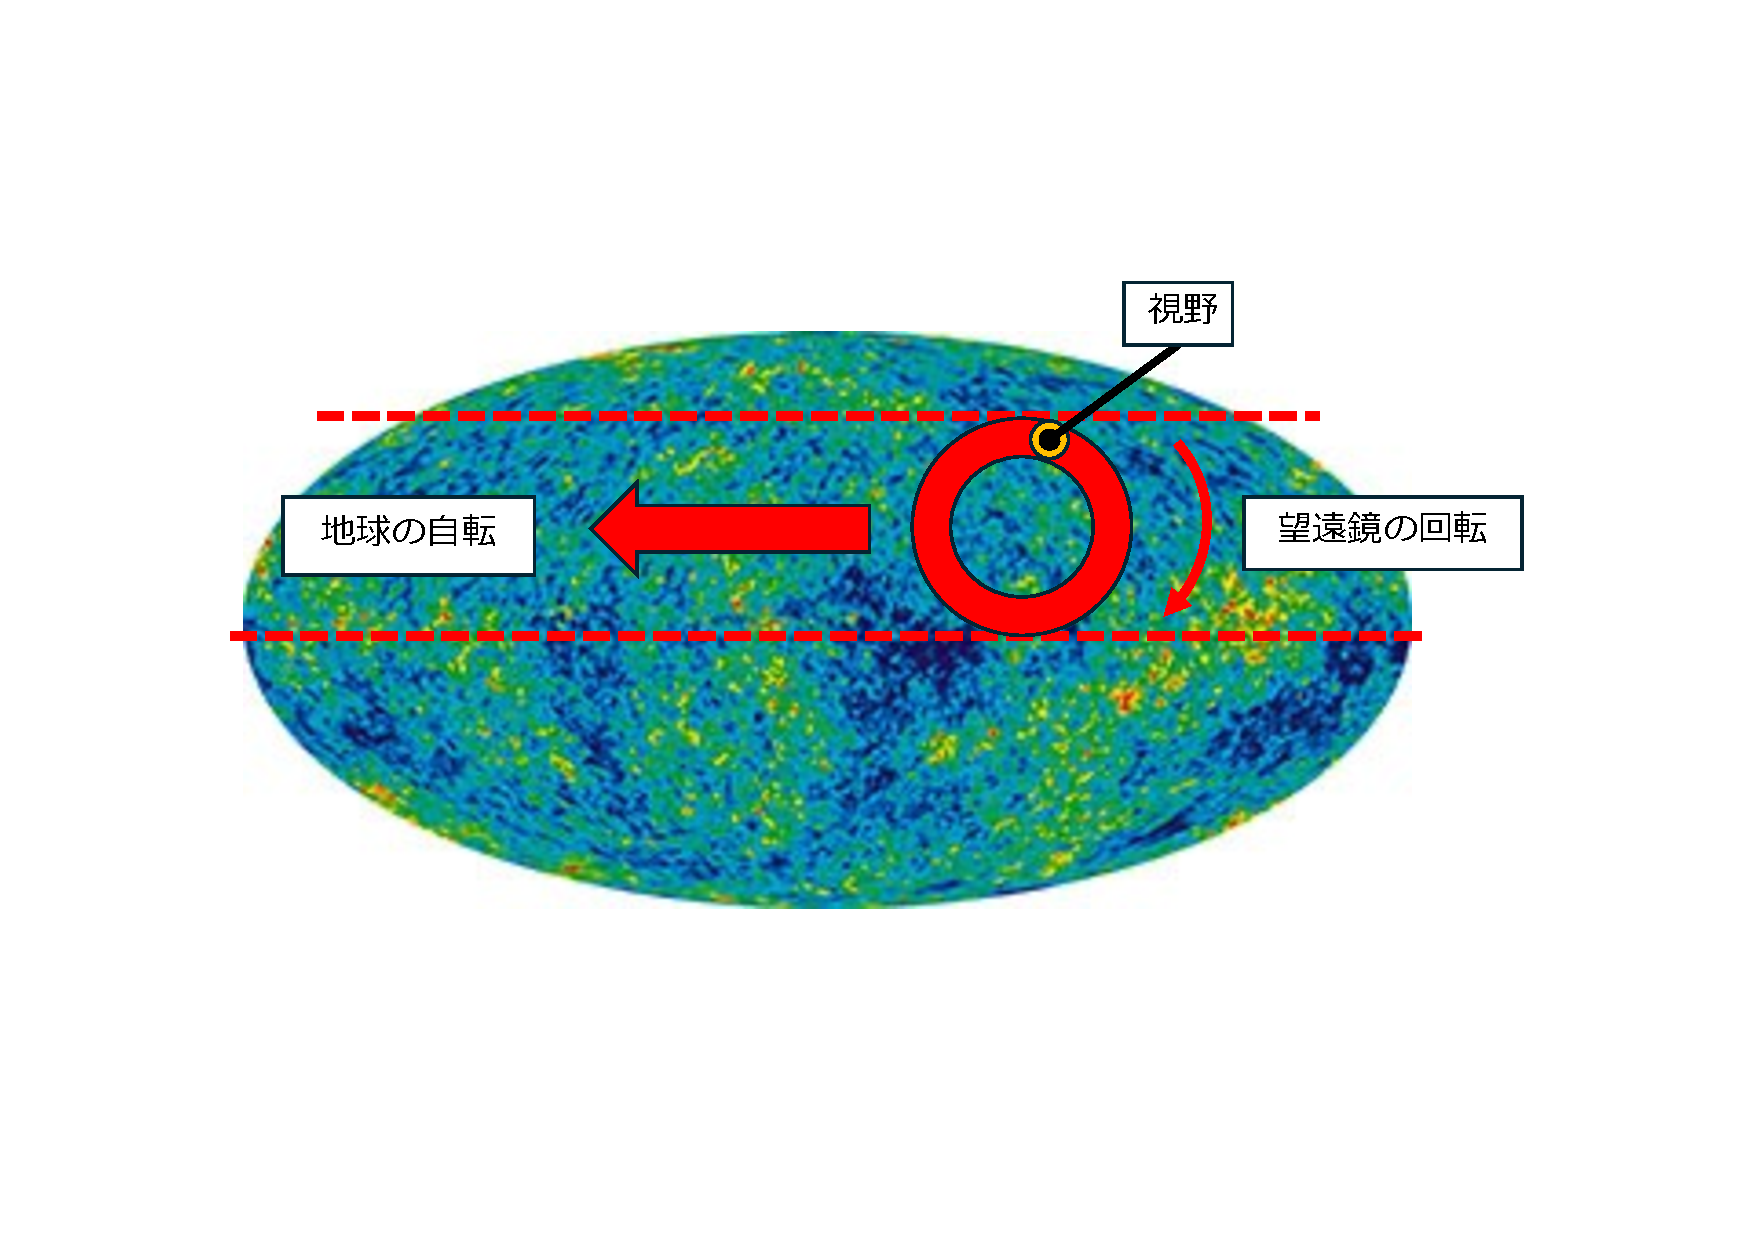
\includegraphics[width=0.8\columnwidth]{3_GB/figs/scan_strategy.pdf}
  \caption{GroundBIRDのスキャン戦略。GroundBIRDは視野$\pm 11^{\circ}$で観測する。望遠鏡の回転と地球の自転を組み合わせることで1日で全天の約半分をカバーできる。}
  \label{scan_strategy}
\end{figure}

次に、GroundBIRDの内部構造の概略を図\ref{GB_inside}に示す。光学系は放物面の主鏡と双曲面の副鏡から成り、CMBがバッフルから入り、光学系で2回反射させた後に、焦点面検出器ステージに入る。クライオスタット内は真空かつ低温になっており、外側のチャンバー部(300K)、40Kシールド、4Kシールドの3層から構成されている。4Kシールドの冷却にはパルスチューブ冷凍機を使用している。GroundBIRDでは超伝導検出器``MKID(Microwave Kinetic Inductance Detector)''を採用しているため、焦点面の温度は極低温に保つ必要がある。焦点面の冷却にはHeソープション冷凍機を使用し、温度を280mK付近に保持している。

\begin{figure}[htbp]
  \centering
  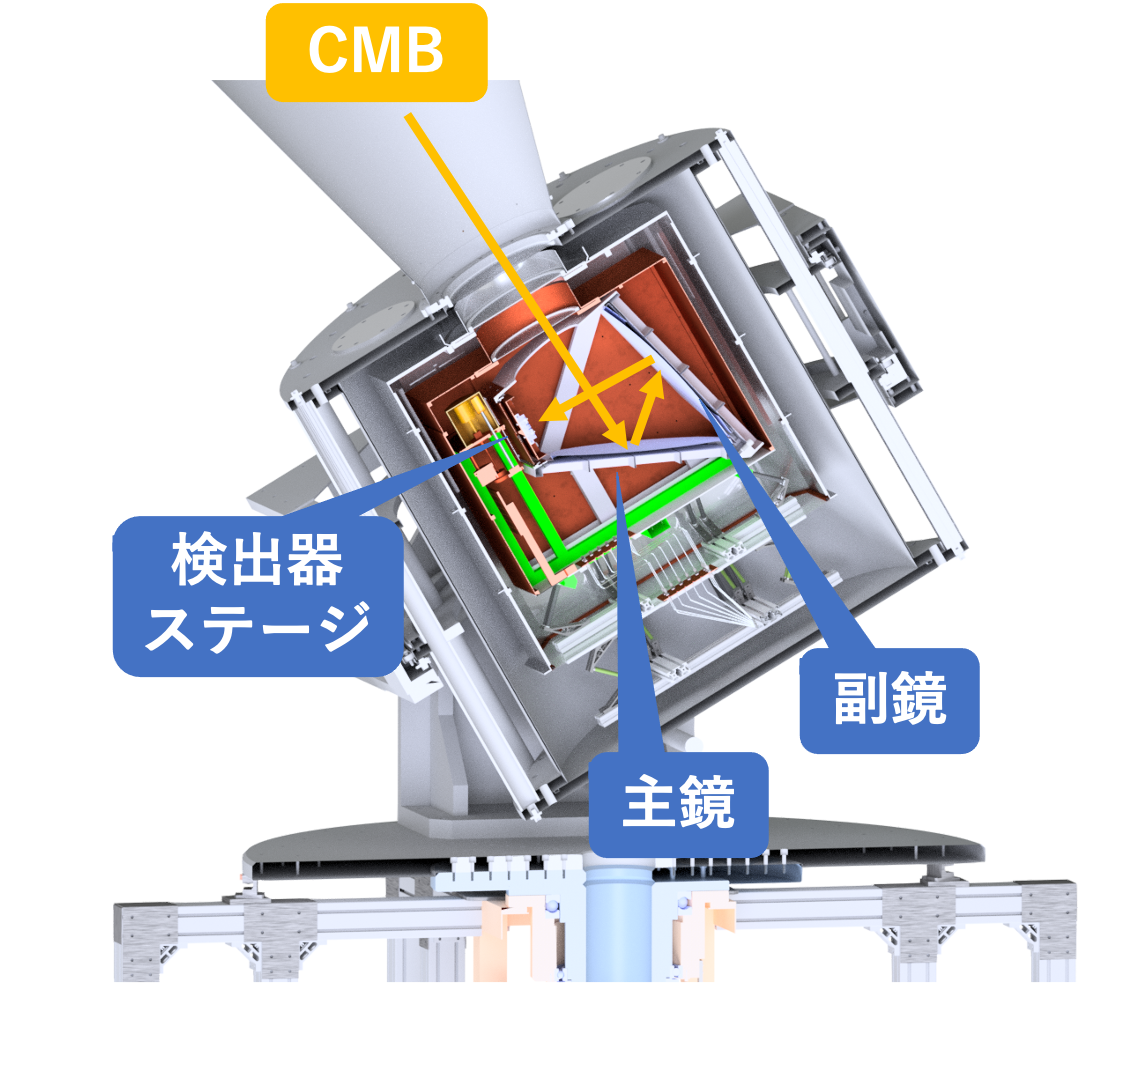
\includegraphics[width=0.6\columnwidth]{3_GB/figs/gb_int.png}
  \caption{GroundBIRD内部の概略図。バッフルを通ってCMBが望遠鏡内に入り、主鏡と副鏡で反射されて検出器ステージに入る。}
  \label{GB_inside}
\end{figure}

\subsection{超伝導検出器MKID}
GroundBIRDでは高速スキャンのもとで角度分解能を失わないようにサンプリングレートを1kHzにしている。そのため、検出器の応答時間が$< \mathcal{O}$(1)msであることが要求される。MKIDの典型的な応答時間は$< \mathcal{O}$(1)msであり\cite{MKID_res}、この要求を満たしている。CMB観測実験では他にも検出器として``TES(Transition Edge Sensor)''ボロメータを使うこともあるが、GroundBIRDでは時間応答性の面からMKIDを採用している。

MKIDの動作原理の概要を説明する。MKIDは超伝導共振回路を応用した高感度な光検出器である。入射する光子のエネルギーに応じて変化する回路内のインダクタンスを、数GHzで読み出す。MKIDの電子顕微鏡写真\cite{MKID_pic}と、等価回路を図\ref{mkid_pic}に示す。MKIDは読み出し線、超伝導体からなる共振器回路、アンテナからなっている。アンテナから電磁波が入射すると超伝導共振器の状態が変化し、そのインピーダンスの変化を読み出すことで入射エネルギーを測定する。具体的には、検出器の温度上昇やエネルギーが$h\nu > 2\Delta$($\Delta$は超伝導ギャップエネルギー)の光子との反応で、超伝導共振器内のクーパー対(結合した電子対)が壊れる。対になっていた電子はエネルギーギャップより上の準位へと押し上げられる(図\ref{cooper})。この過程で生成される電子を準粒子という。準粒子によって共振器内の超伝導状態が変化し、可変インダクタンスの値が変化する。また、1つの読み出し線に複数の共振器が容量性カップリング(Capacitive coupling; Cカップリング)しており、1対の読み出し配線を使って$\mathcal{O}$(1000)個のMKIDを同時に読み出すことができる。

\begin{figure}[h]
  \begin{tabular}{cc}
    %---- 最初の図 ---------------------------
    \begin{minipage}[t]{0.45\hsize}
      \centering
      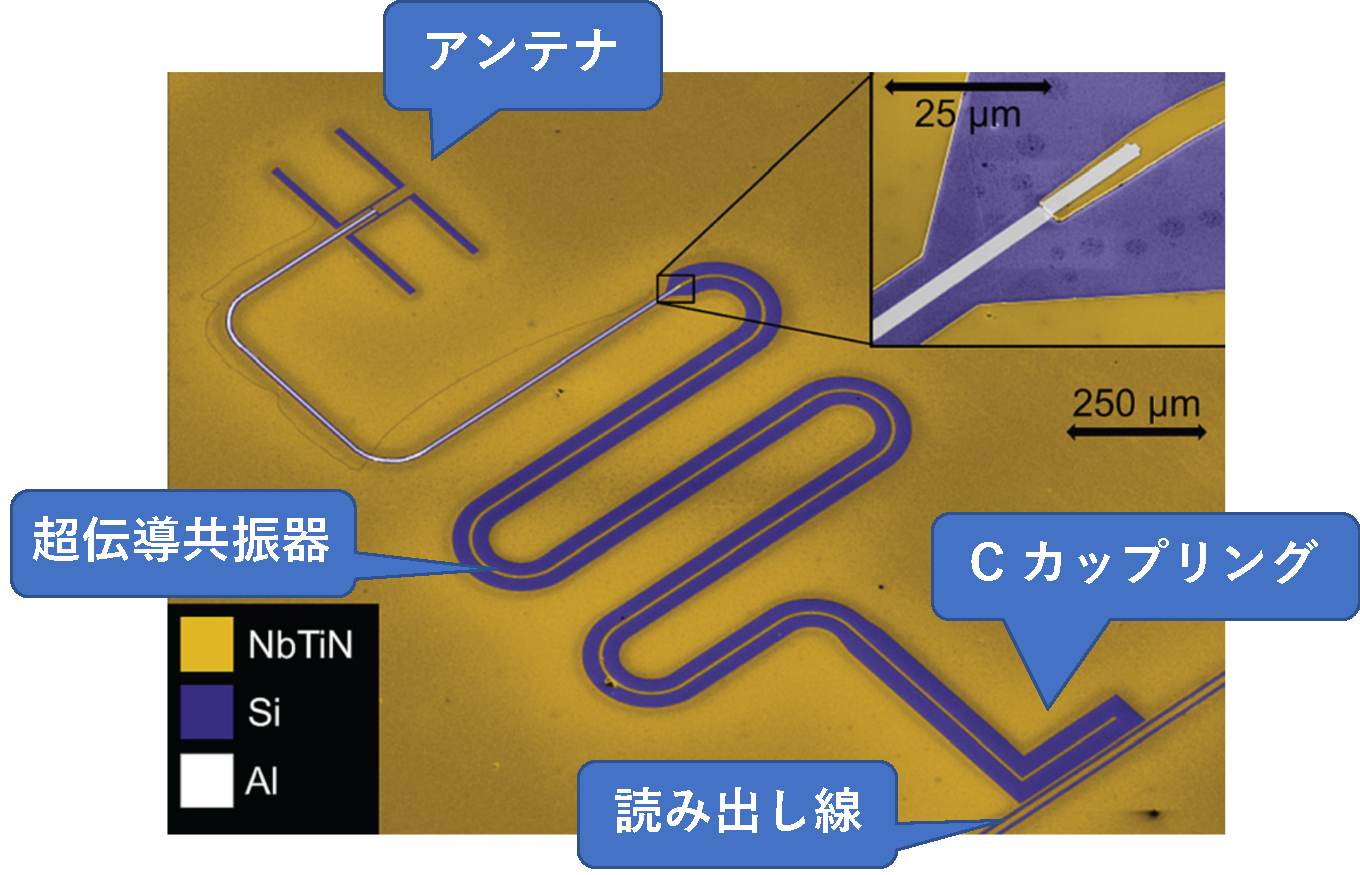
\includegraphics[keepaspectratio, scale=0.3]{3_GB/figs/mkid_pic.pdf}
      \subcaption{MKIDの電子顕微鏡写真\cite{MKID_pic}。読み出し線、超伝導共振器、アンテナからなる。}
    \end{minipage}
    %---- 2番目の図 --------------------------
    \begin{minipage}[t]{0.45\hsize}
      \centering
      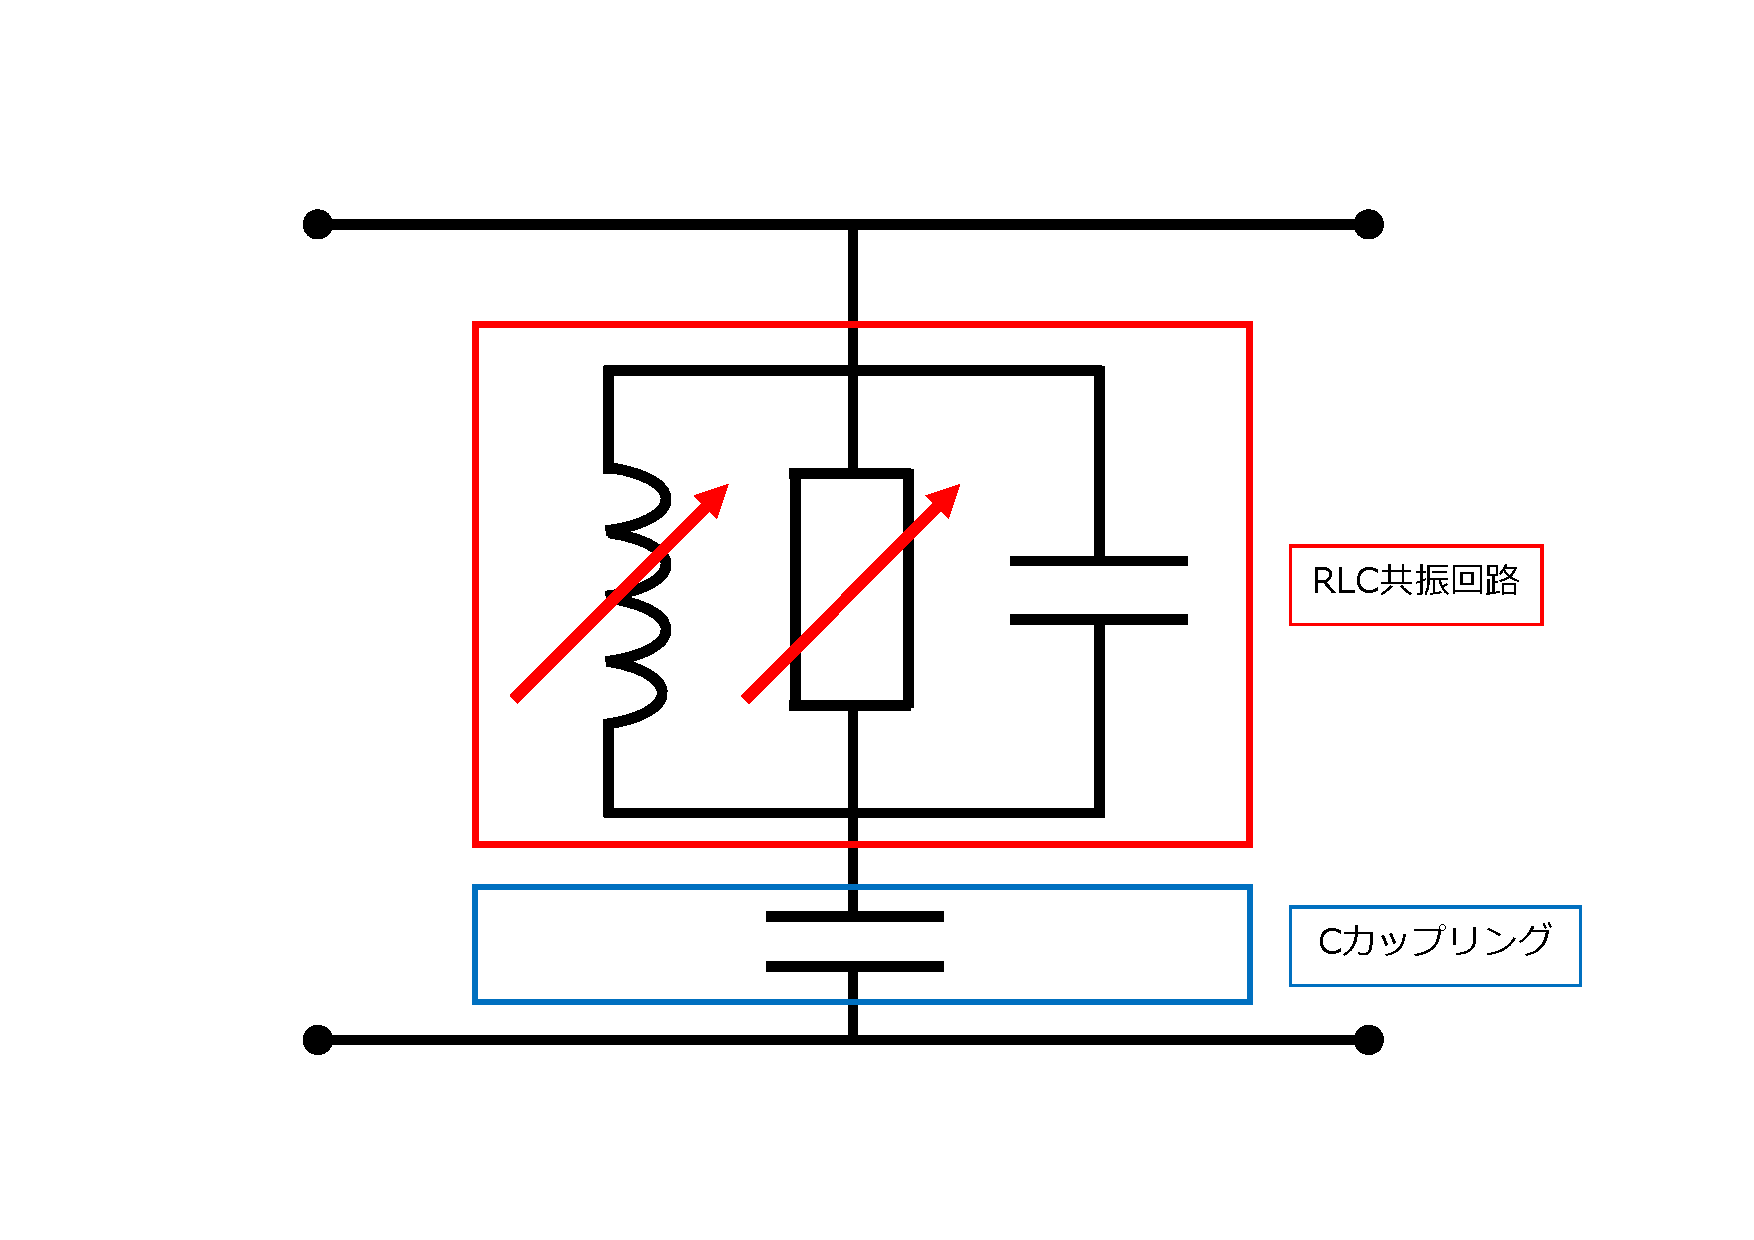
\includegraphics[keepaspectratio, scale=0.3]{3_GB/figs/mkid_circ.pdf}
      \subcaption{MKIDの等価回路。可変インダクタンスと可変抵抗をもつRLC共振回路になっている。}
    \end{minipage}
    %---- 図はここまで ----------------------
  \end{tabular}
  \caption{超伝導検出器MKID}
  \label{mkid_pic}
\end{figure}

\begin{figure}[htbp]
  \centering
  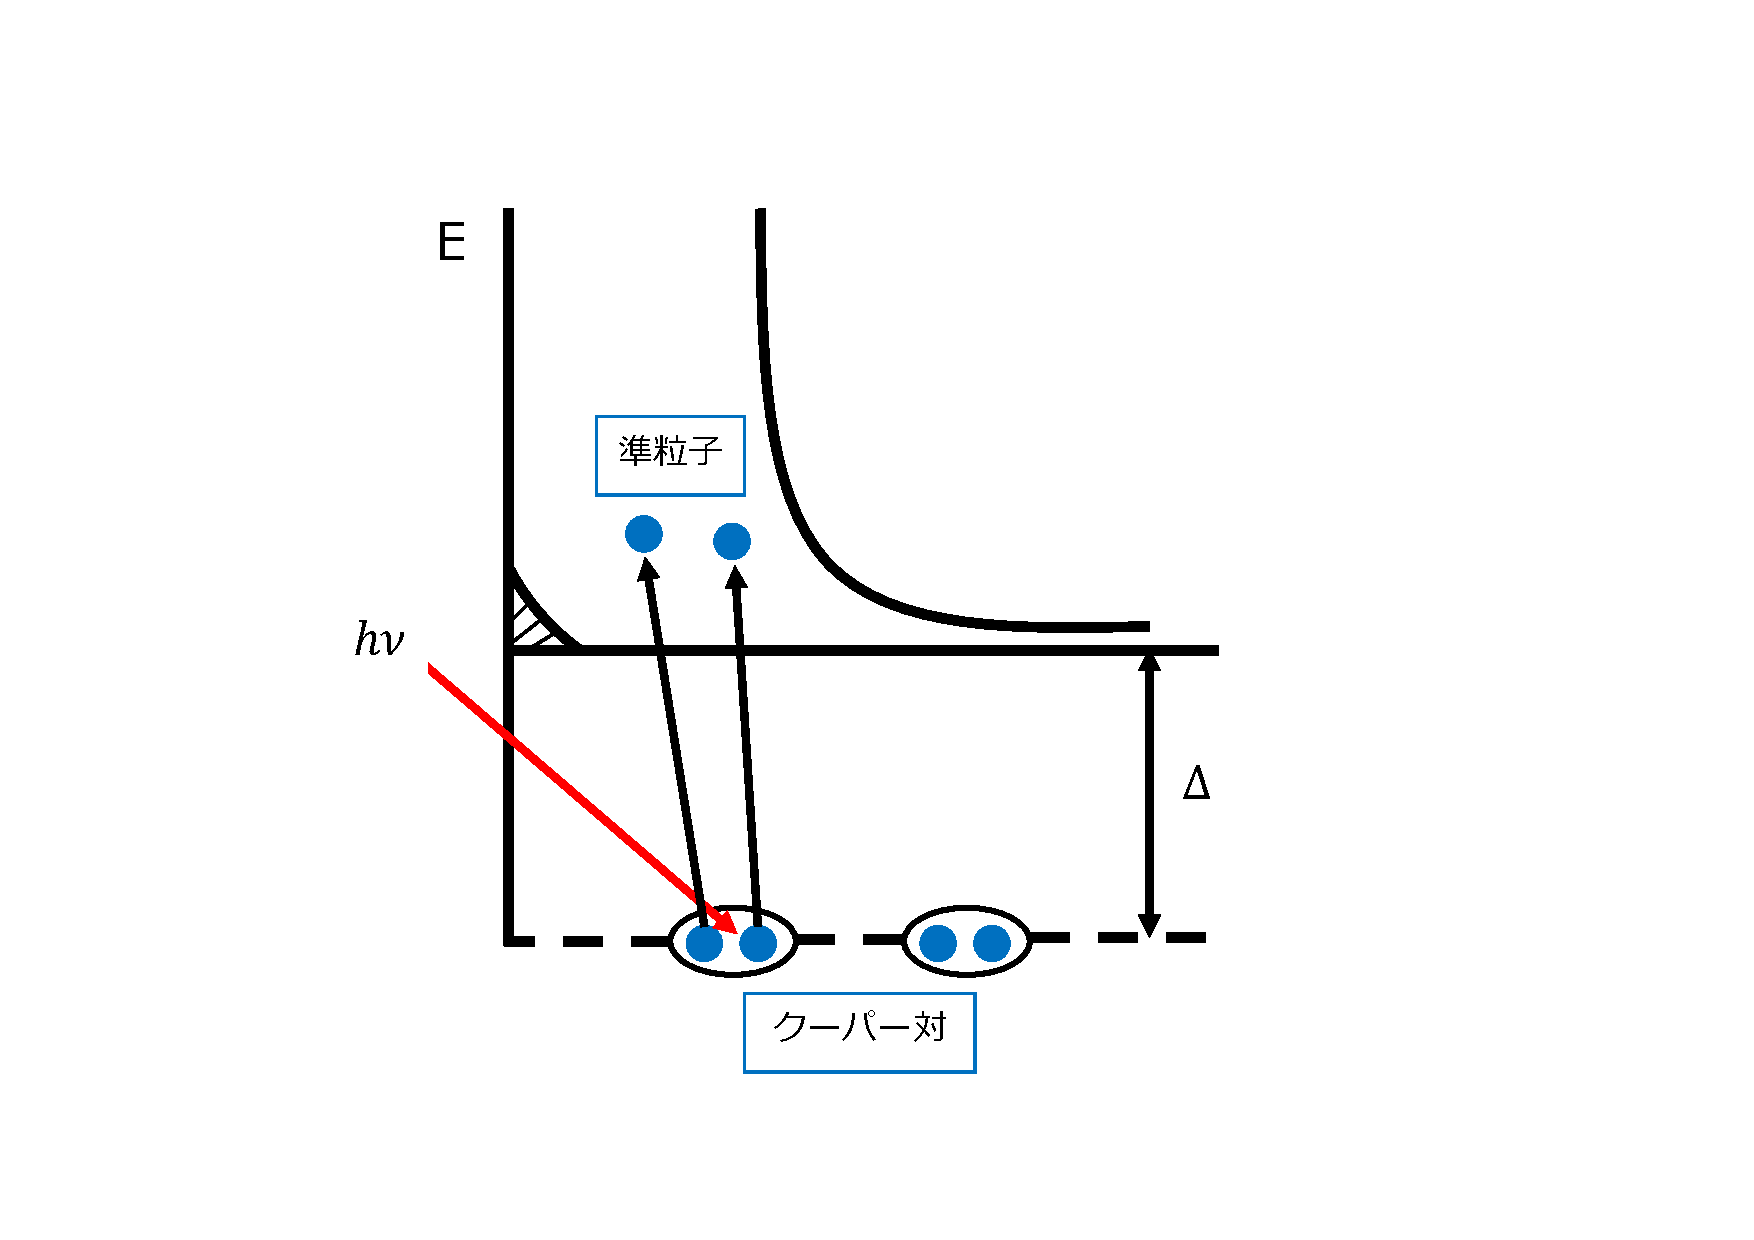
\includegraphics[width=0.6\columnwidth]{3_GB/figs/cooper.pdf}
  \caption{入射光子による準粒子生成の模式図。縦軸は電子のエネルギーを表す。$h\nu > 2\Delta$のエネルギーを持つ光が超伝導共振器に入射すると、クーパー対が壊されてエネルギー準位が押し上げられ、準粒子になる。}
  \label{cooper}
\end{figure}

\subsection{物理ターゲット}
GroundBIRDが探る物理ターゲットは\ref{E_and_tau}で見た光学的厚み$\tau$の地上からの再測定である。光学的厚み$\tau$の測定は今までにWMAPやPlanckといった衛星実験によって測定がされてきた。図\ref{tau_planck}に測定された$\tau$の値の変遷を示す。誤差が小さくなってきており、最新の測定結果ではその誤差は$\sim 10\%$である。しかし、平均値は系統的に下がっている傾向にあり、独立した測定によってこの結果の妥当性を評価する必要がある。そのため、地上実験(例えばCLASS\cite{CLASS}やQUIJOTE\cite{QUIJOTE}など)からの$\tau$の精密測定が始まっている。

\begin{figure}[htbp]
  \centering
  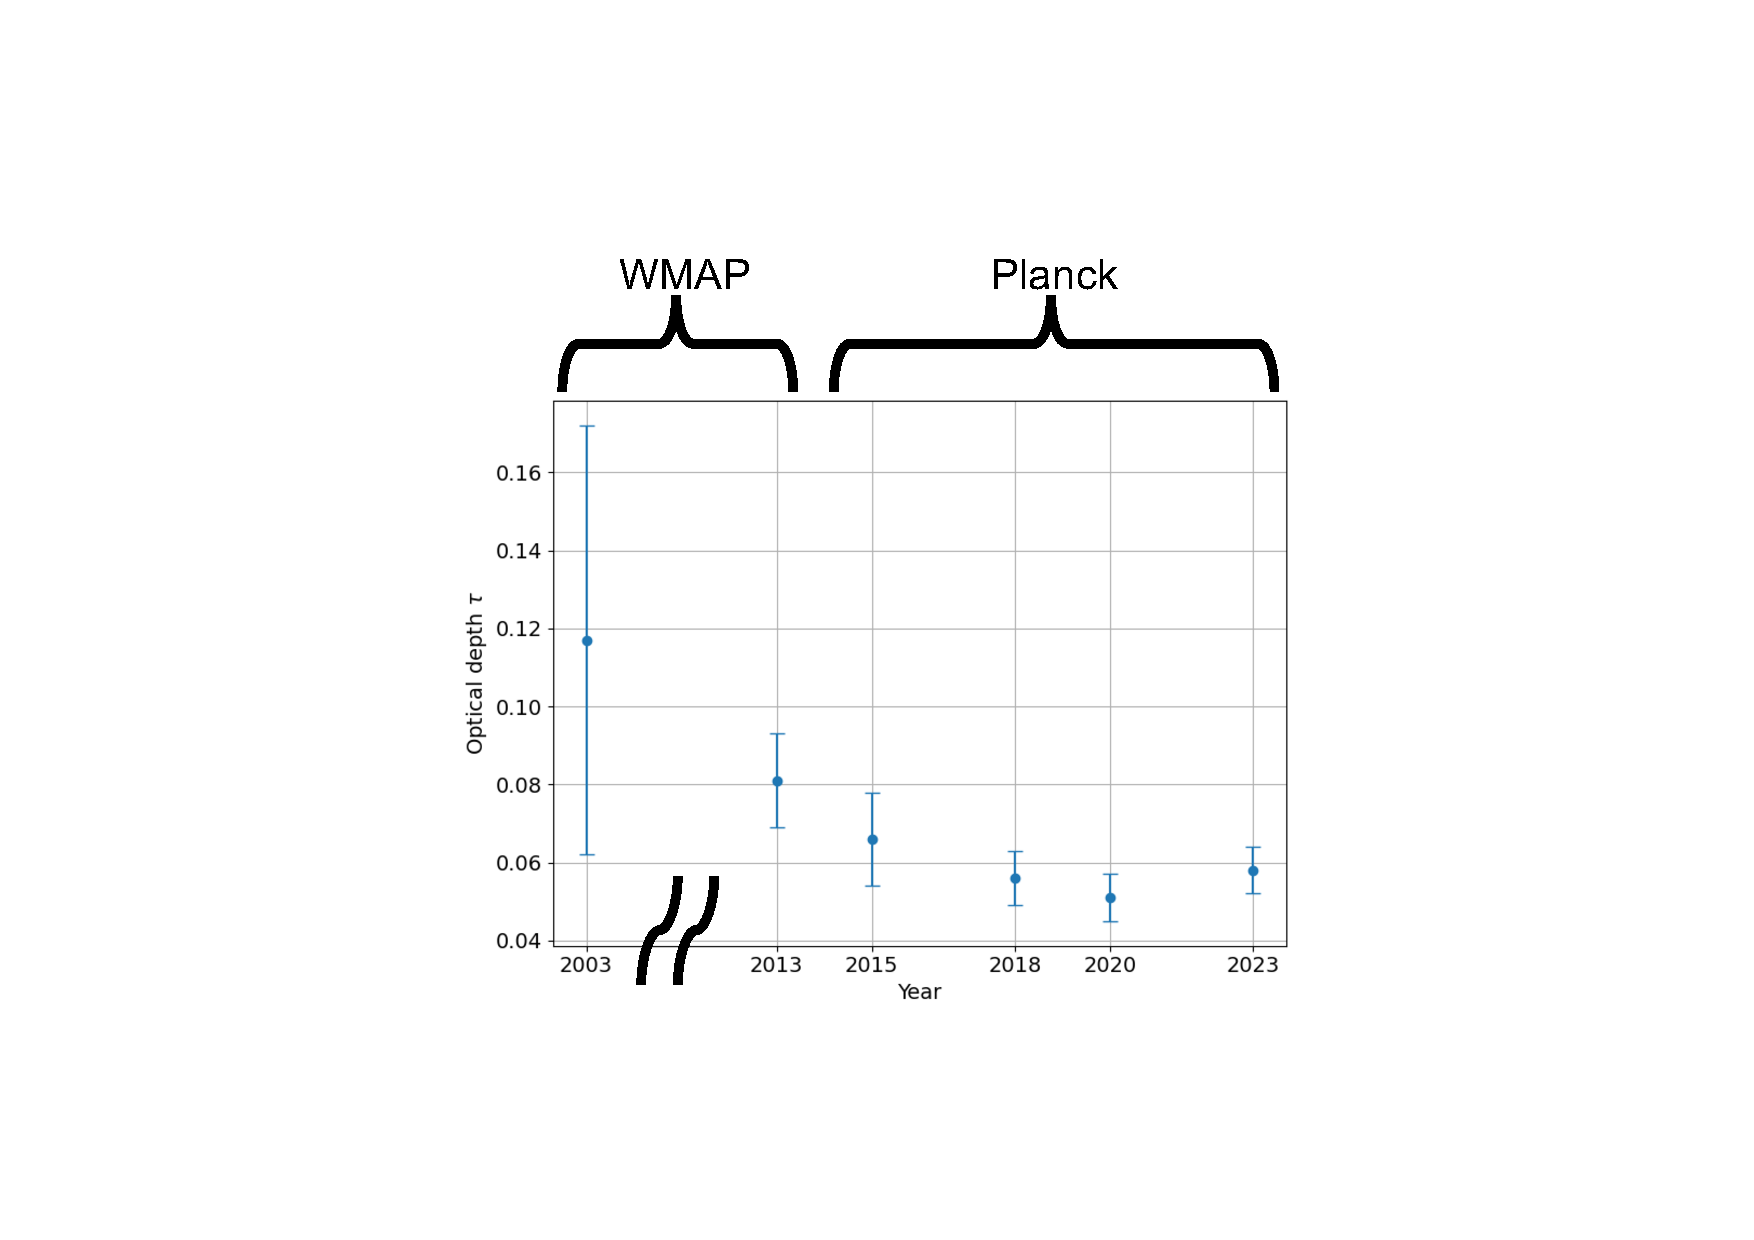
\includegraphics[width=0.8\columnwidth]{3_GB/figs/tau_planck_wmap_cut.pdf}
  \caption{WMAPとPlanckによって測定された光学的厚み$\tau$の値\cite{tau_measure}。最新では誤差は$\sim 10\%$である。}
  \label{tau_planck}
\end{figure}

特にGroundBIRDは独自のスキャン戦略を活かして$\tau$の値に迫ることができる。高速スキャンによって大角度スケール(6 $<\ell<$ 300)のCMB偏光を測定することができる。大角度スケールと$\tau$の関係を図\ref{cl_honda}に示す。偏光Eモードのパワースペクトルは大角度スケール($\geq 10^{\circ}$)で$\tau$に応じて異なる振る舞いをする。GroundBIRDはこの振る舞いを観測することができるため、$\tau$の測定に適している。

\begin{figure}[htbp]
  \centering
  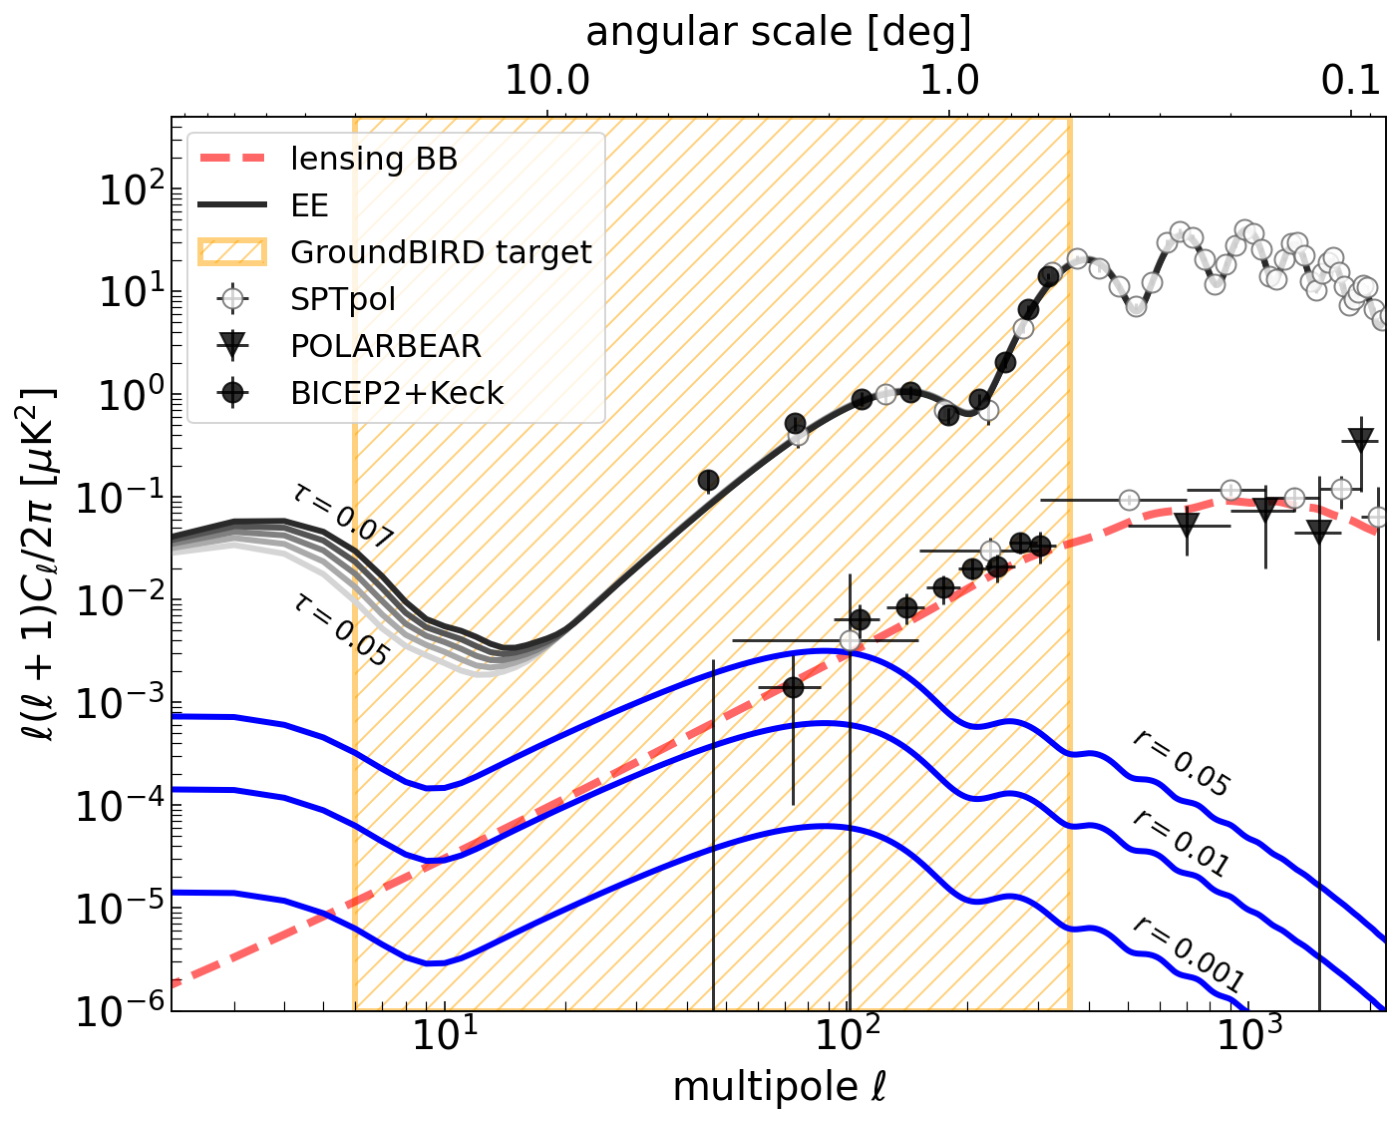
\includegraphics[width=0.8\columnwidth]{3_GB/figs/cl_shonda.pdf}
  \caption{パワースペクトルの過去の観測結果とE,Bモードの理論線、そしてGroundBIRDの観測領域\cite{spie_honda}をオレンジで示す。青実線はテンソル$\cdot$スカラー比を仮定した時の原始重力波由来の偏光Bモード、赤点線は重力レンズ効果由来のBモードを表す。黒実線はEモードであり、大角度スケール($\geq 10^{\circ}$)で$\tau$の値によってスペクトルに違いが生まれる。}
  \label{cl_honda}
\end{figure}

CMB偏光の観測から$\tau$の測定を行うためにはCMBと、銀河などから来るCMBと同周波数帯の放射である``前景放射''とを分離する必要がある。これらの前景放射はそれぞれ異なる周波数依存性を持つ(図\ref{planck_spectrum})。主な前景放射には低周波側で卓越する``シンクロトロン放射''と高周波側で卓越する``ダスト熱放射''があり、CMBにとって大きなノイズとなる。そのため、低周波側$\mathcal{O}$(10)GHzから高周波側$\mathcal{O}$(100)GHzまでの広い帯域での観測を行い前景放射を取り除くことが求められる。\ref{full_array}で述べるが、GroundBIRDはCMBに感度のある145GHzと、ダスト放射に感度がある220GHzの2つの帯域で観測する。一方で、低周波側はQUIJOTE\footnote{QUIJOTE実験はGroundBIRDから20mほどしか離れていない隣に位置する望遠鏡である。}のデータを使うことでカバーする。3年間の観測で、GroundBIRDとQUIJOTEの共同解析によって$\tau$を誤差$\sigma_{\tau}\sim$ 0.01で測定することを目指す\cite{joint_ana}。

\begin{figure}[htbp]
  \centering
  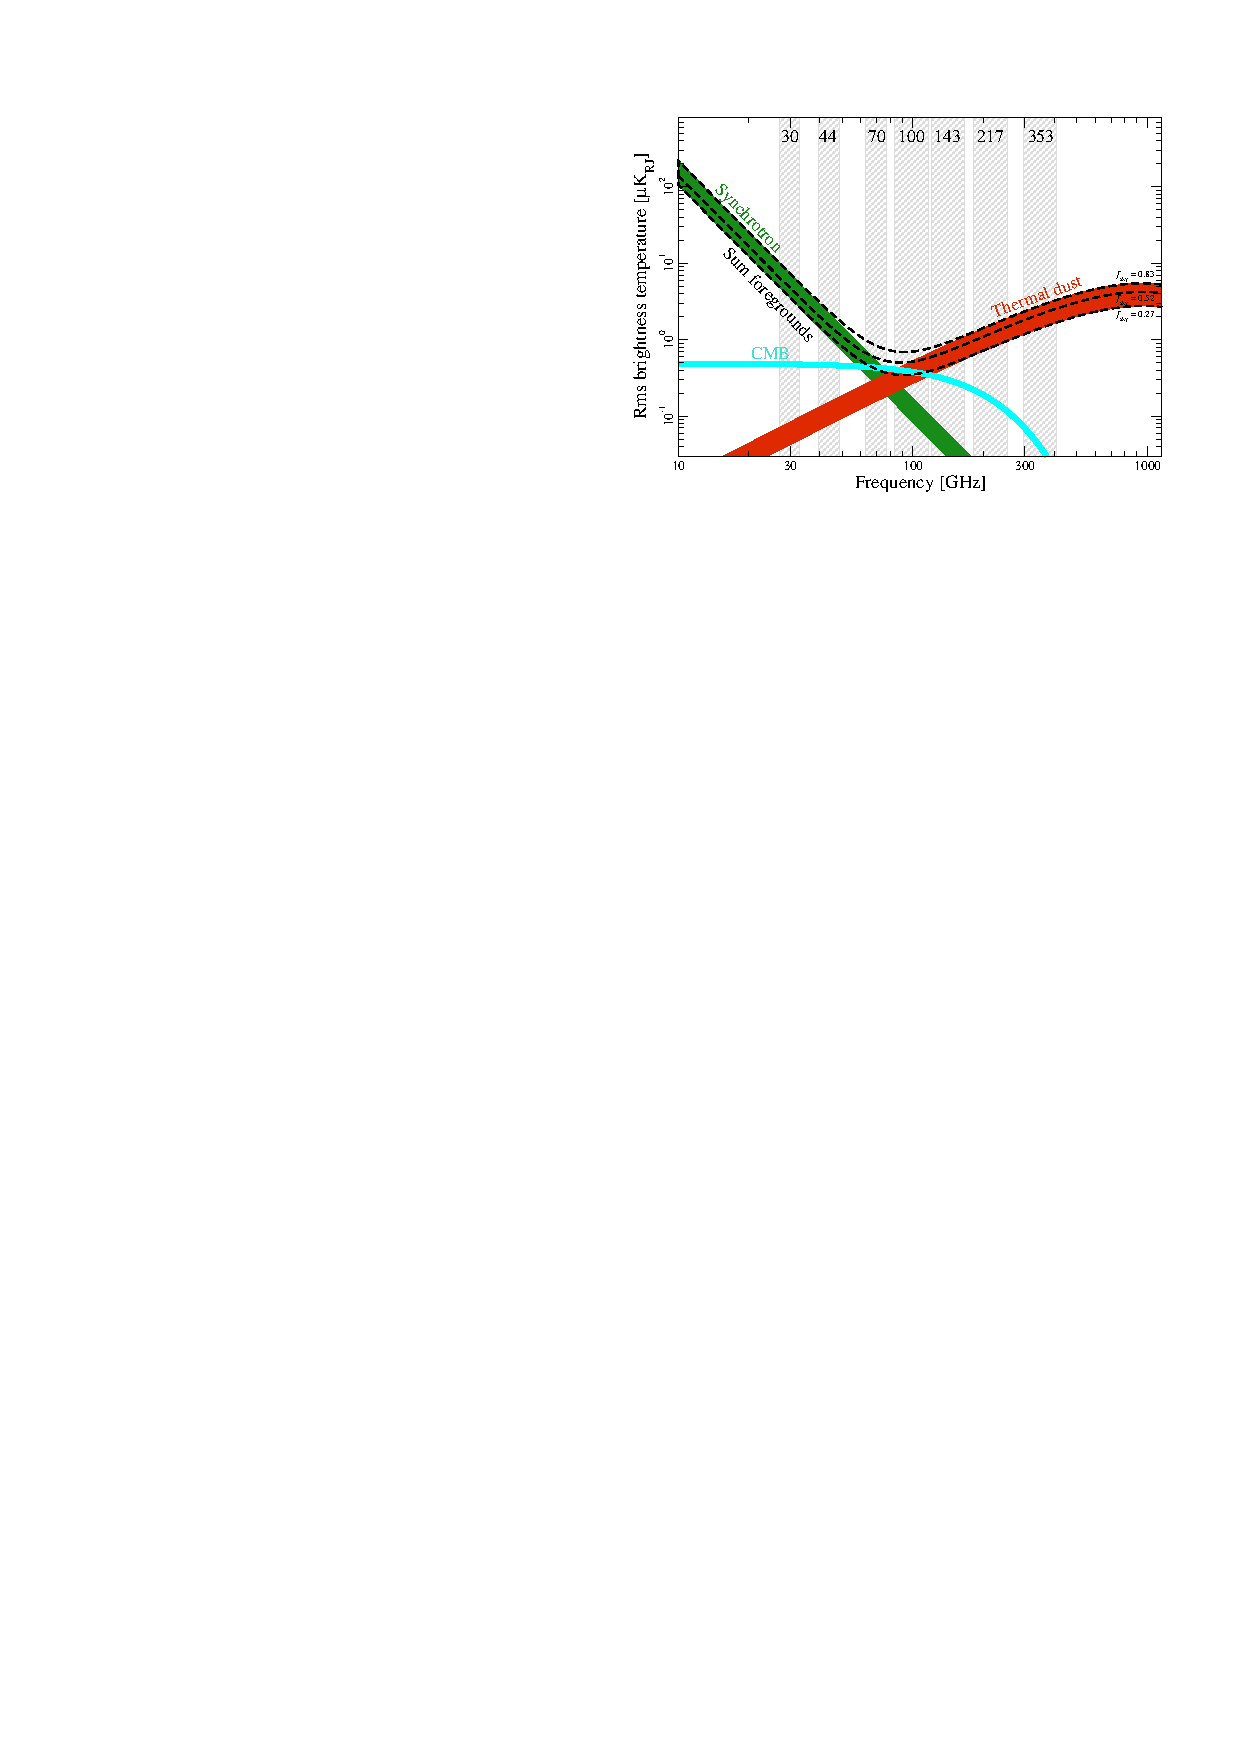
\includegraphics[width=0.8\columnwidth]{3_GB/figs/planck_spectrum.pdf}
  \caption{CMBと前景放射の偏光強度を周波数の関数として表した図。Planck\cite{planck_cmb}を参照。それぞれの前景放射は異なる周波数依存性を持ち、CMBとこれらを分離するためには広い帯域での観測が必要になる。}
  \label{planck_spectrum}
\end{figure}

\section{現在の観測状況}

\subsection{検出器のフルアレイインストール}
\label{full_array}
GroundBIRDの現在の状況について説明する。2022年1月から2022年5月まではプロトタイプ検出器を用いたコミッショニング観測が行われた。コミッショニングデータを用いて望遠鏡の視線方向の較正\cite{sueno_paper}や、偏光角較正、ノイズ特性の理解\cite{sueno_doctor}などがされてきた。並行して、2023年5月に全焦点面検出器のインストールが完了し、本格的な物理観測がスタートした。インストールした焦点面検出器を図\ref{full_array_mkid}に示す。複数のMKIDが1つのアレイに搭載されており、145GHzが6アレイと220GHzが1アレイの全7アレイからなる。中央に220GHzアレイがあり、その周りを145GHzアレイが囲むように並んでいる。アレイごとに読み出しを行う。アレイ内でのMKIDの配置は図\ref{mkid_design}にようになっている。

\begin{figure}[h]
  \begin{tabular}{cc}
    %---- 最初の図 ---------------------------
    \begin{minipage}[t]{0.45\hsize}
      \centering
      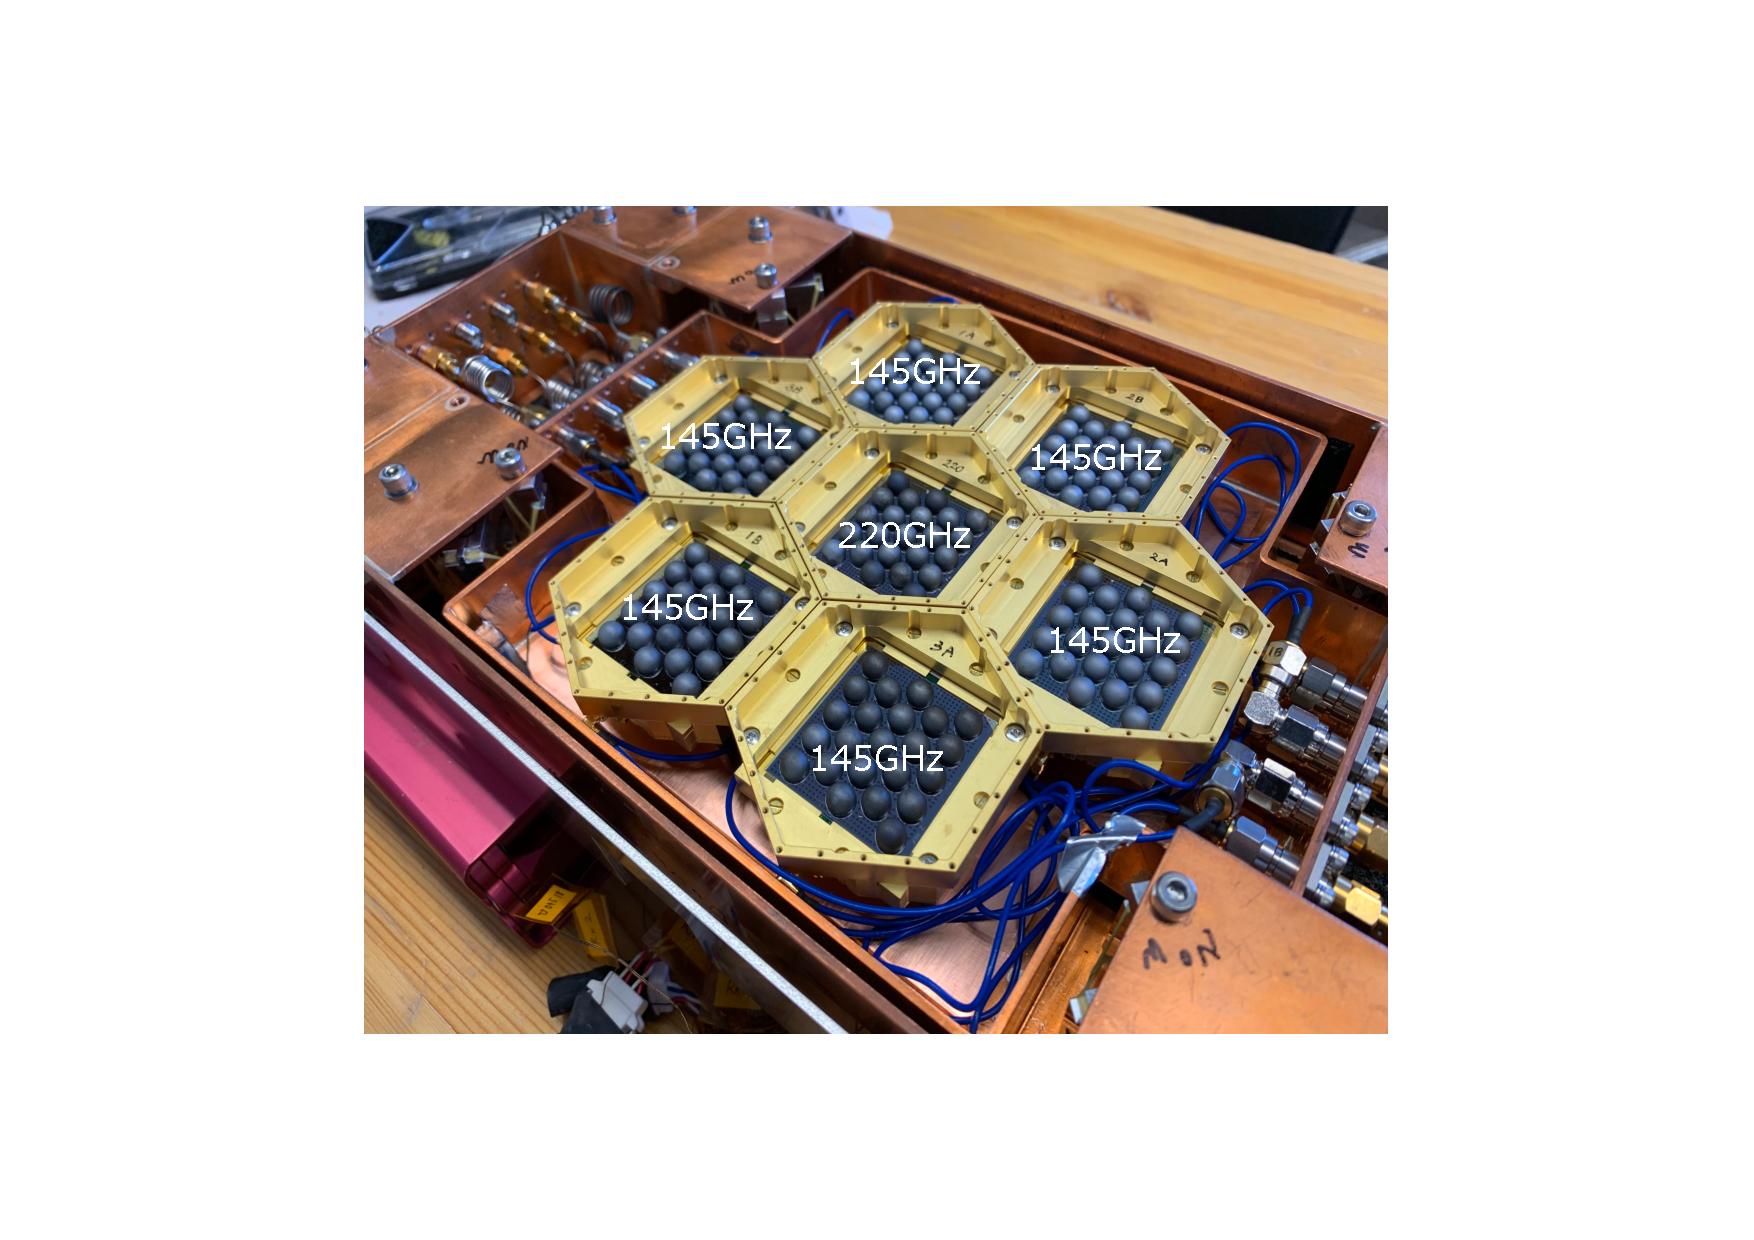
\includegraphics[keepaspectratio, scale=0.37]{3_GB/figs/full_array.pdf}
      \subcaption{焦点面検出器の全体写真。}
    \end{minipage}
    %---- 2番目の図 --------------------------
    \begin{minipage}[t]{0.45\hsize}
      \centering
      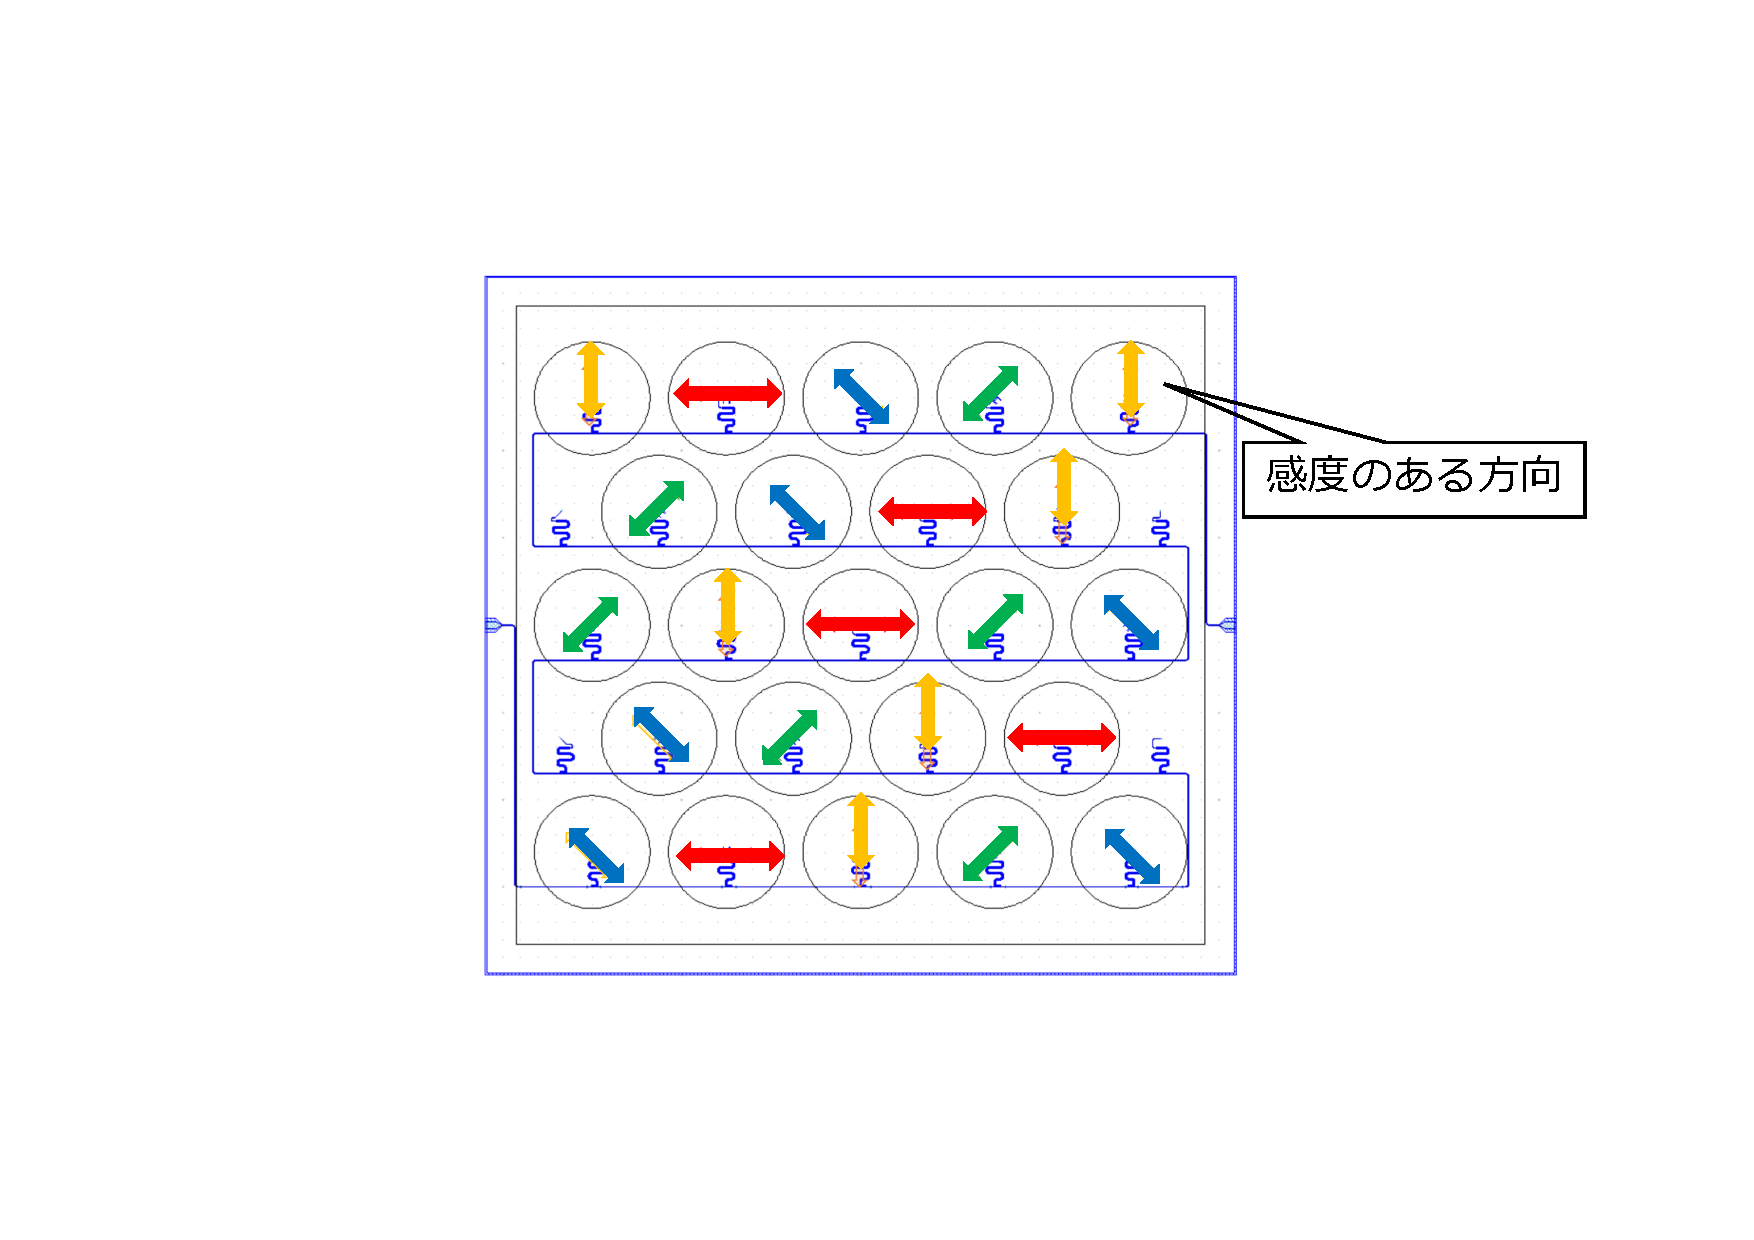
\includegraphics[keepaspectratio, scale=0.43]{3_GB/figs/mkid_design.pdf}
      \subcaption{アレイ内のMKIDが感度を持つ偏光方向。}
      \label{mkid_design}
    \end{minipage}
    %---- 図はここまで ----------------------
  \end{tabular}
  \caption{フルアレイの焦点面検出器MKID}
  \label{full_array_mkid}
\end{figure}

\subsection{リモート観測システム}

\section{本論文の構成}
ここまで第\ref{chapter1}章でCMBに関わる理論的な背景、第\ref{chapter2}章でGroundBIRDの概要を説明した。以降は第\ref{chapter3}章と第\ref{chapter4}章の2部構成になっており、第\ref{chapter3}章でGroundBIRDの角度データ取得システムの改善について、第\ref{chapter4}章で焦点面検出器のアライメント較正とその結果について述べる。第\ref{chapter5}章で今後の展望を述べ、第\ref{chapter6}章でまとめを述べる。

\chapter{仰角データ取得システムの改善}
\label{chapter3}

CMB観測においては、検出器の時系列データと望遠鏡の角度データを途切れることなく連続的に取得し続けなければいけない。そのため、角度データ取得システムは安定的でかつ操作性がよいものであることが求められる。本章では既存の望遠鏡の仰角データ取得システムを改善し、その動作確認を行なった。
\section{望遠鏡仰角データ取得システムの改善}

\subsection{角度情報データ取得の概要}
はじめに、GroundBIRD全体でのデータ取得システムの概要を述べる。CMB観測においては検出器の信号を時系列データ(以下、TODと略す)として取得する。最終的なマップ作成のためには、TODと同期して望遠鏡の視線情報(角度データ)を取得することが求められる。GroundBIRDでは望遠鏡の仰角方向と方位角方向で2つの角度データを取得している。連続回転する回転台の上部と下部は回転継手\cite{rotary_joint}によって電気的に接続されている(図\ref{GB_daq})。

\begin{figure}[htbp]
  \centering
  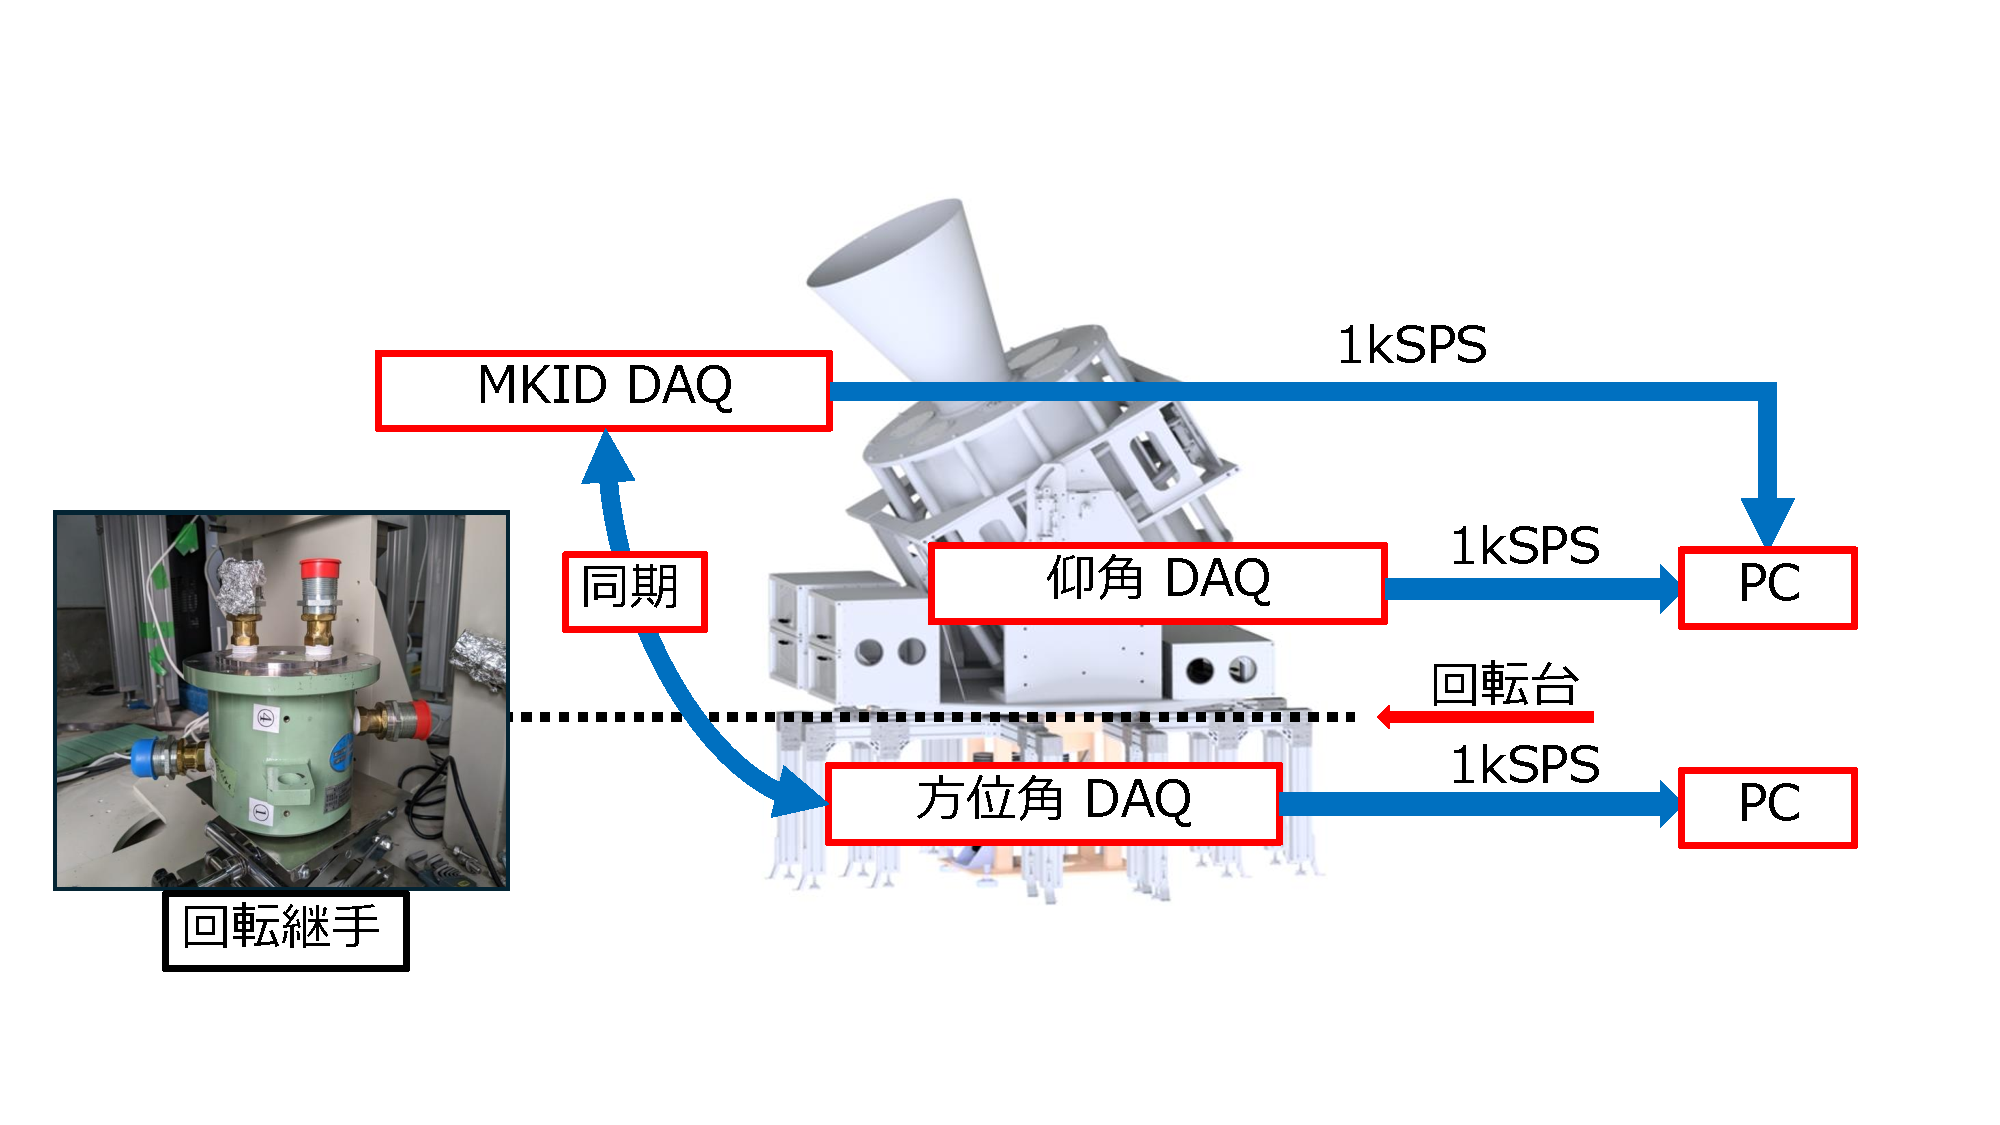
\includegraphics[width=1.0\columnwidth]{4_elDAQ/figs/GB_daq_2.pdf}
  \caption{GroundBIRDの検出器データと角度データ取得系の概要。回転する回転台の上下での信号同期は``回転継手''が担っている。}
  \label{GB_daq}
\end{figure}

仰角方向の角度データは、望遠鏡の側面に取り付けられたロータリーエンコーダー(Canon, R-1SL \cite{R-1SL})を使用し、Digilent製のFPGAボードZybo Z7-20 (\cite{Zybo}、以下では単にZyboと記す)で読み出す(図\ref{el_daq})。FPGAとはField Programmable Gate Array の略で、様々な論理回路がチップに搭載されており、使用者が配線を自由に組み合わせて論理回路を作ることができるデバイスである。FPGAでは特定の演算を行う回路を作成できるため、高速処理を可能にする。また並列処理も得意である。エンコーダーは4秒角($1.1\cdot{10^{-3}}~^{\circ}$)もの高い角度分解能を持つ。

\begin{figure}[h]
  \begin{tabular}{cc}
    %---- 最初の図 ---------------------------
    \begin{minipage}[t]{0.45\hsize}
      \centering
      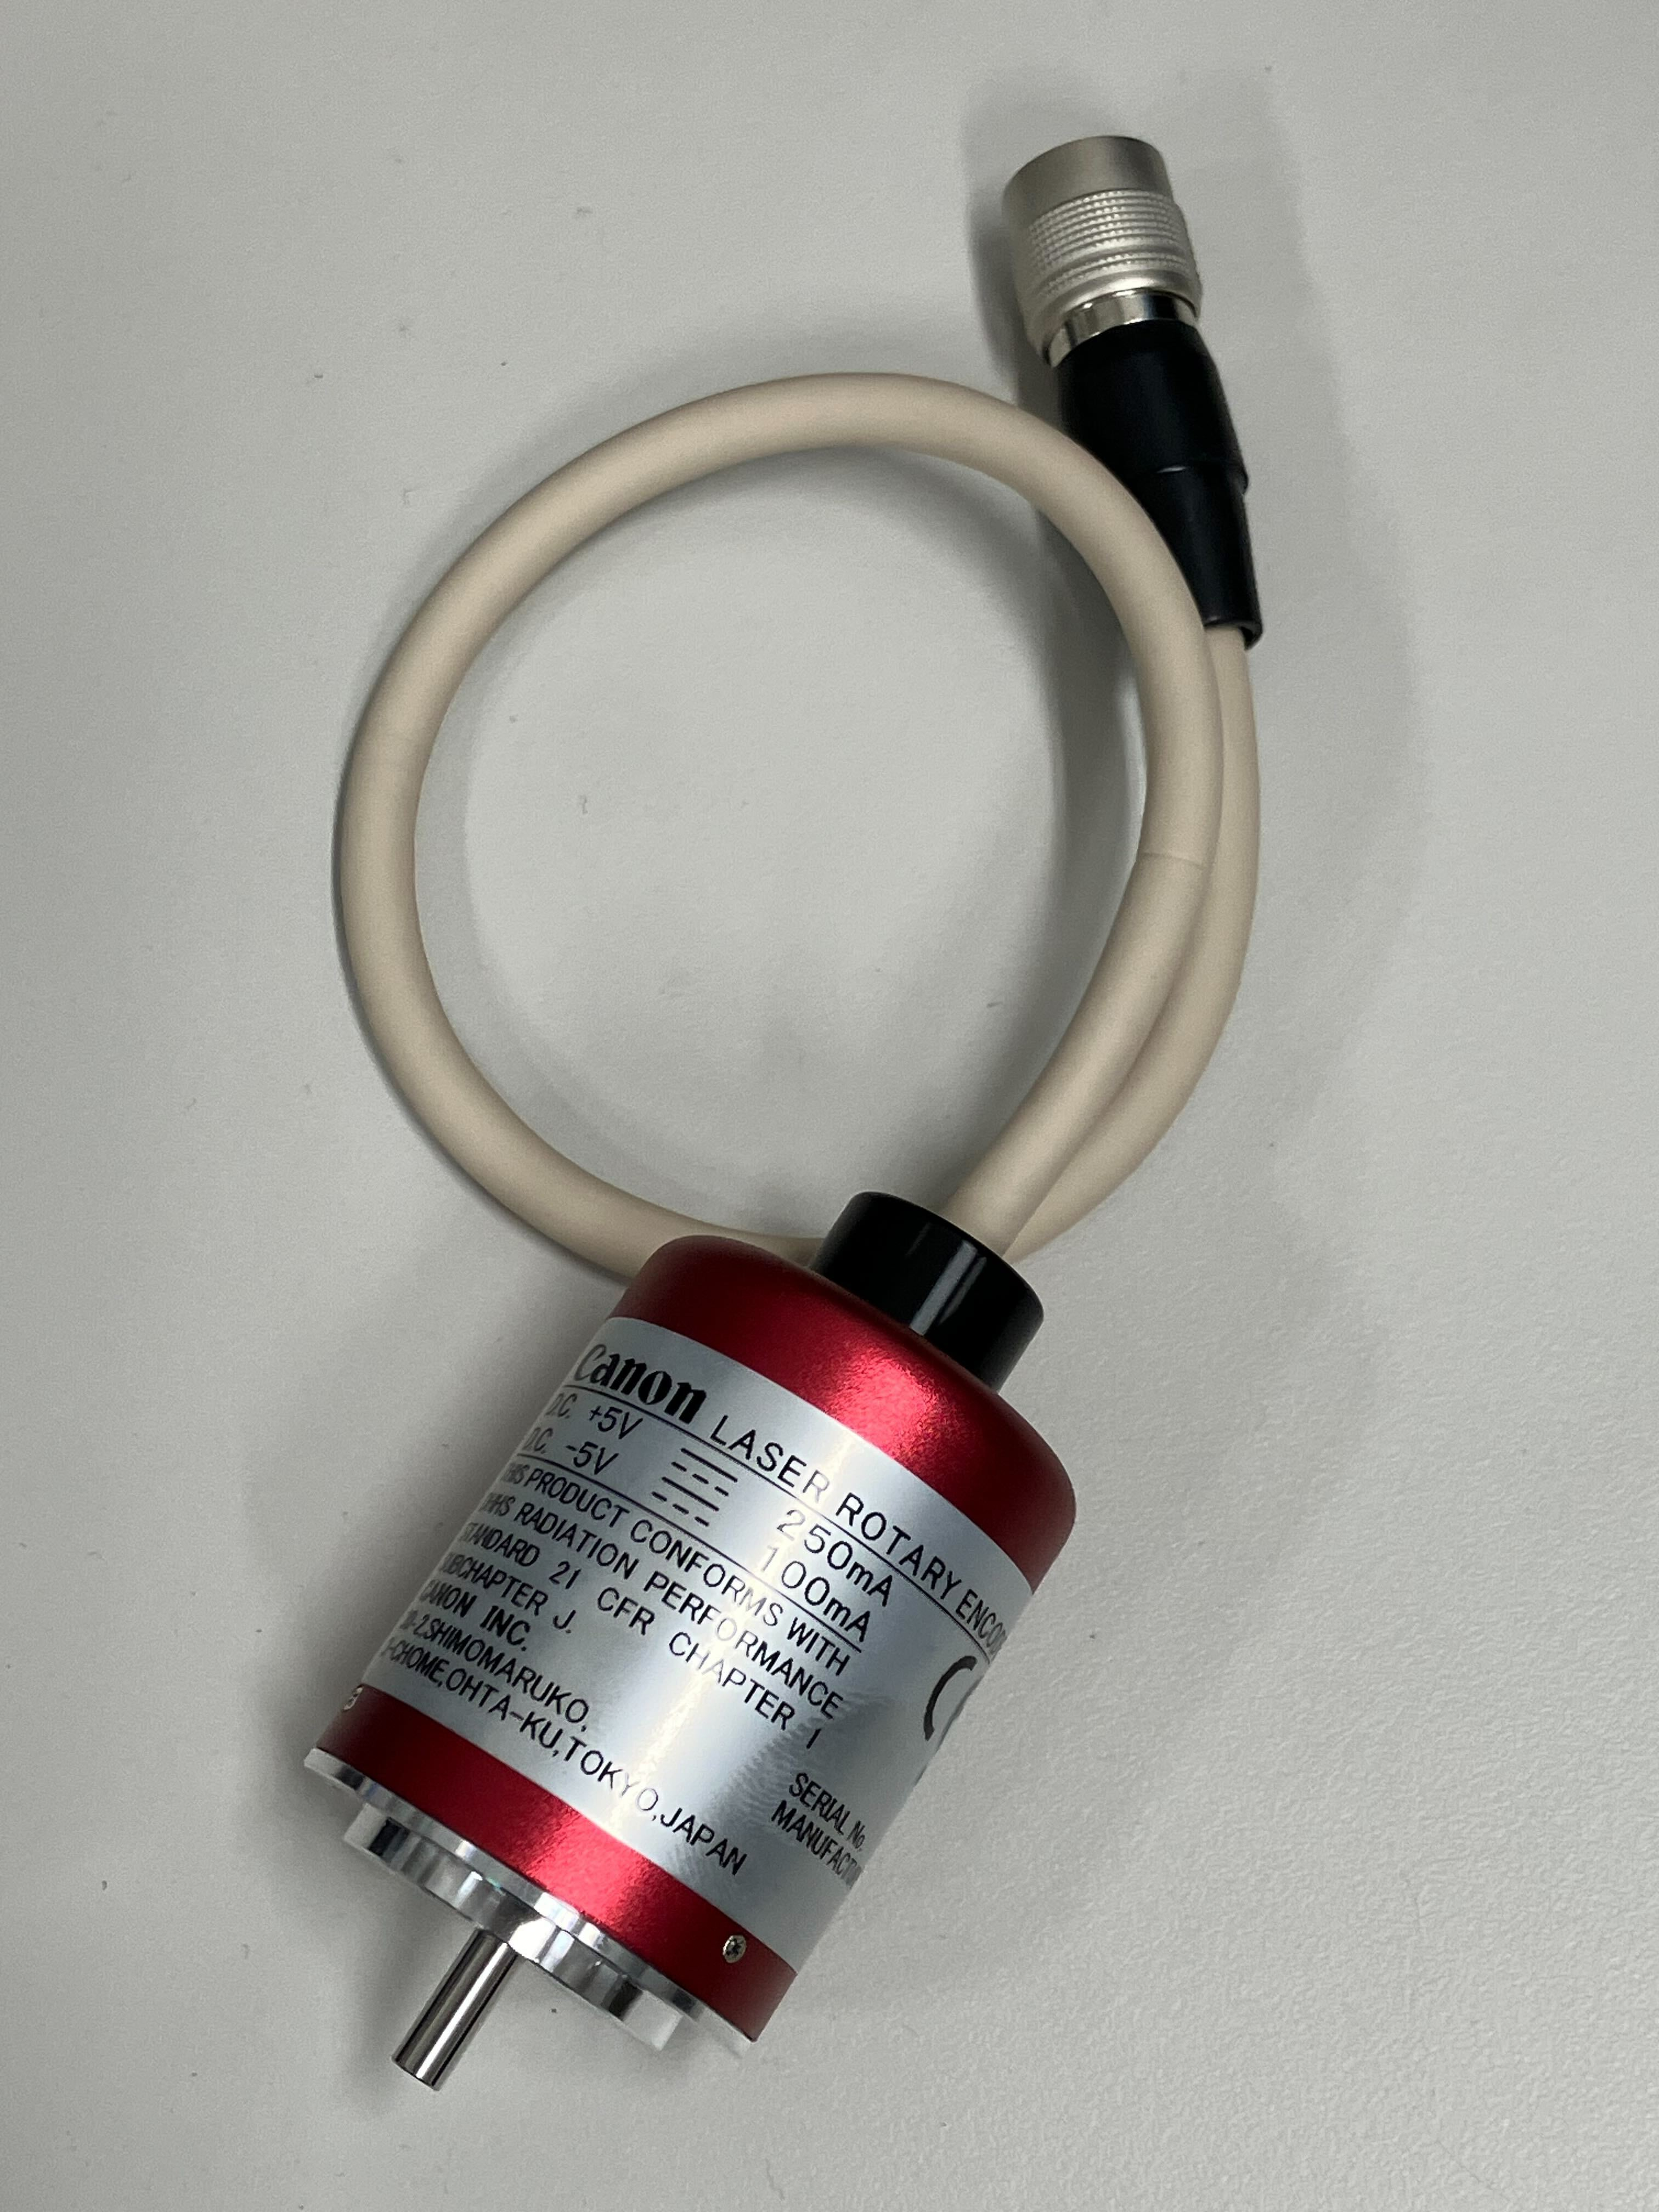
\includegraphics[keepaspectratio, scale=0.04]{4_elDAQ/figs/el_encoder.jpg}
      \subcaption{ロータリーエンコーダー(Canon, R-1SL \cite{R-1SL})}
    \end{minipage}
    %---- 2番目の図 --------------------------
    \begin{minipage}[t]{0.45\hsize}
      \centering
      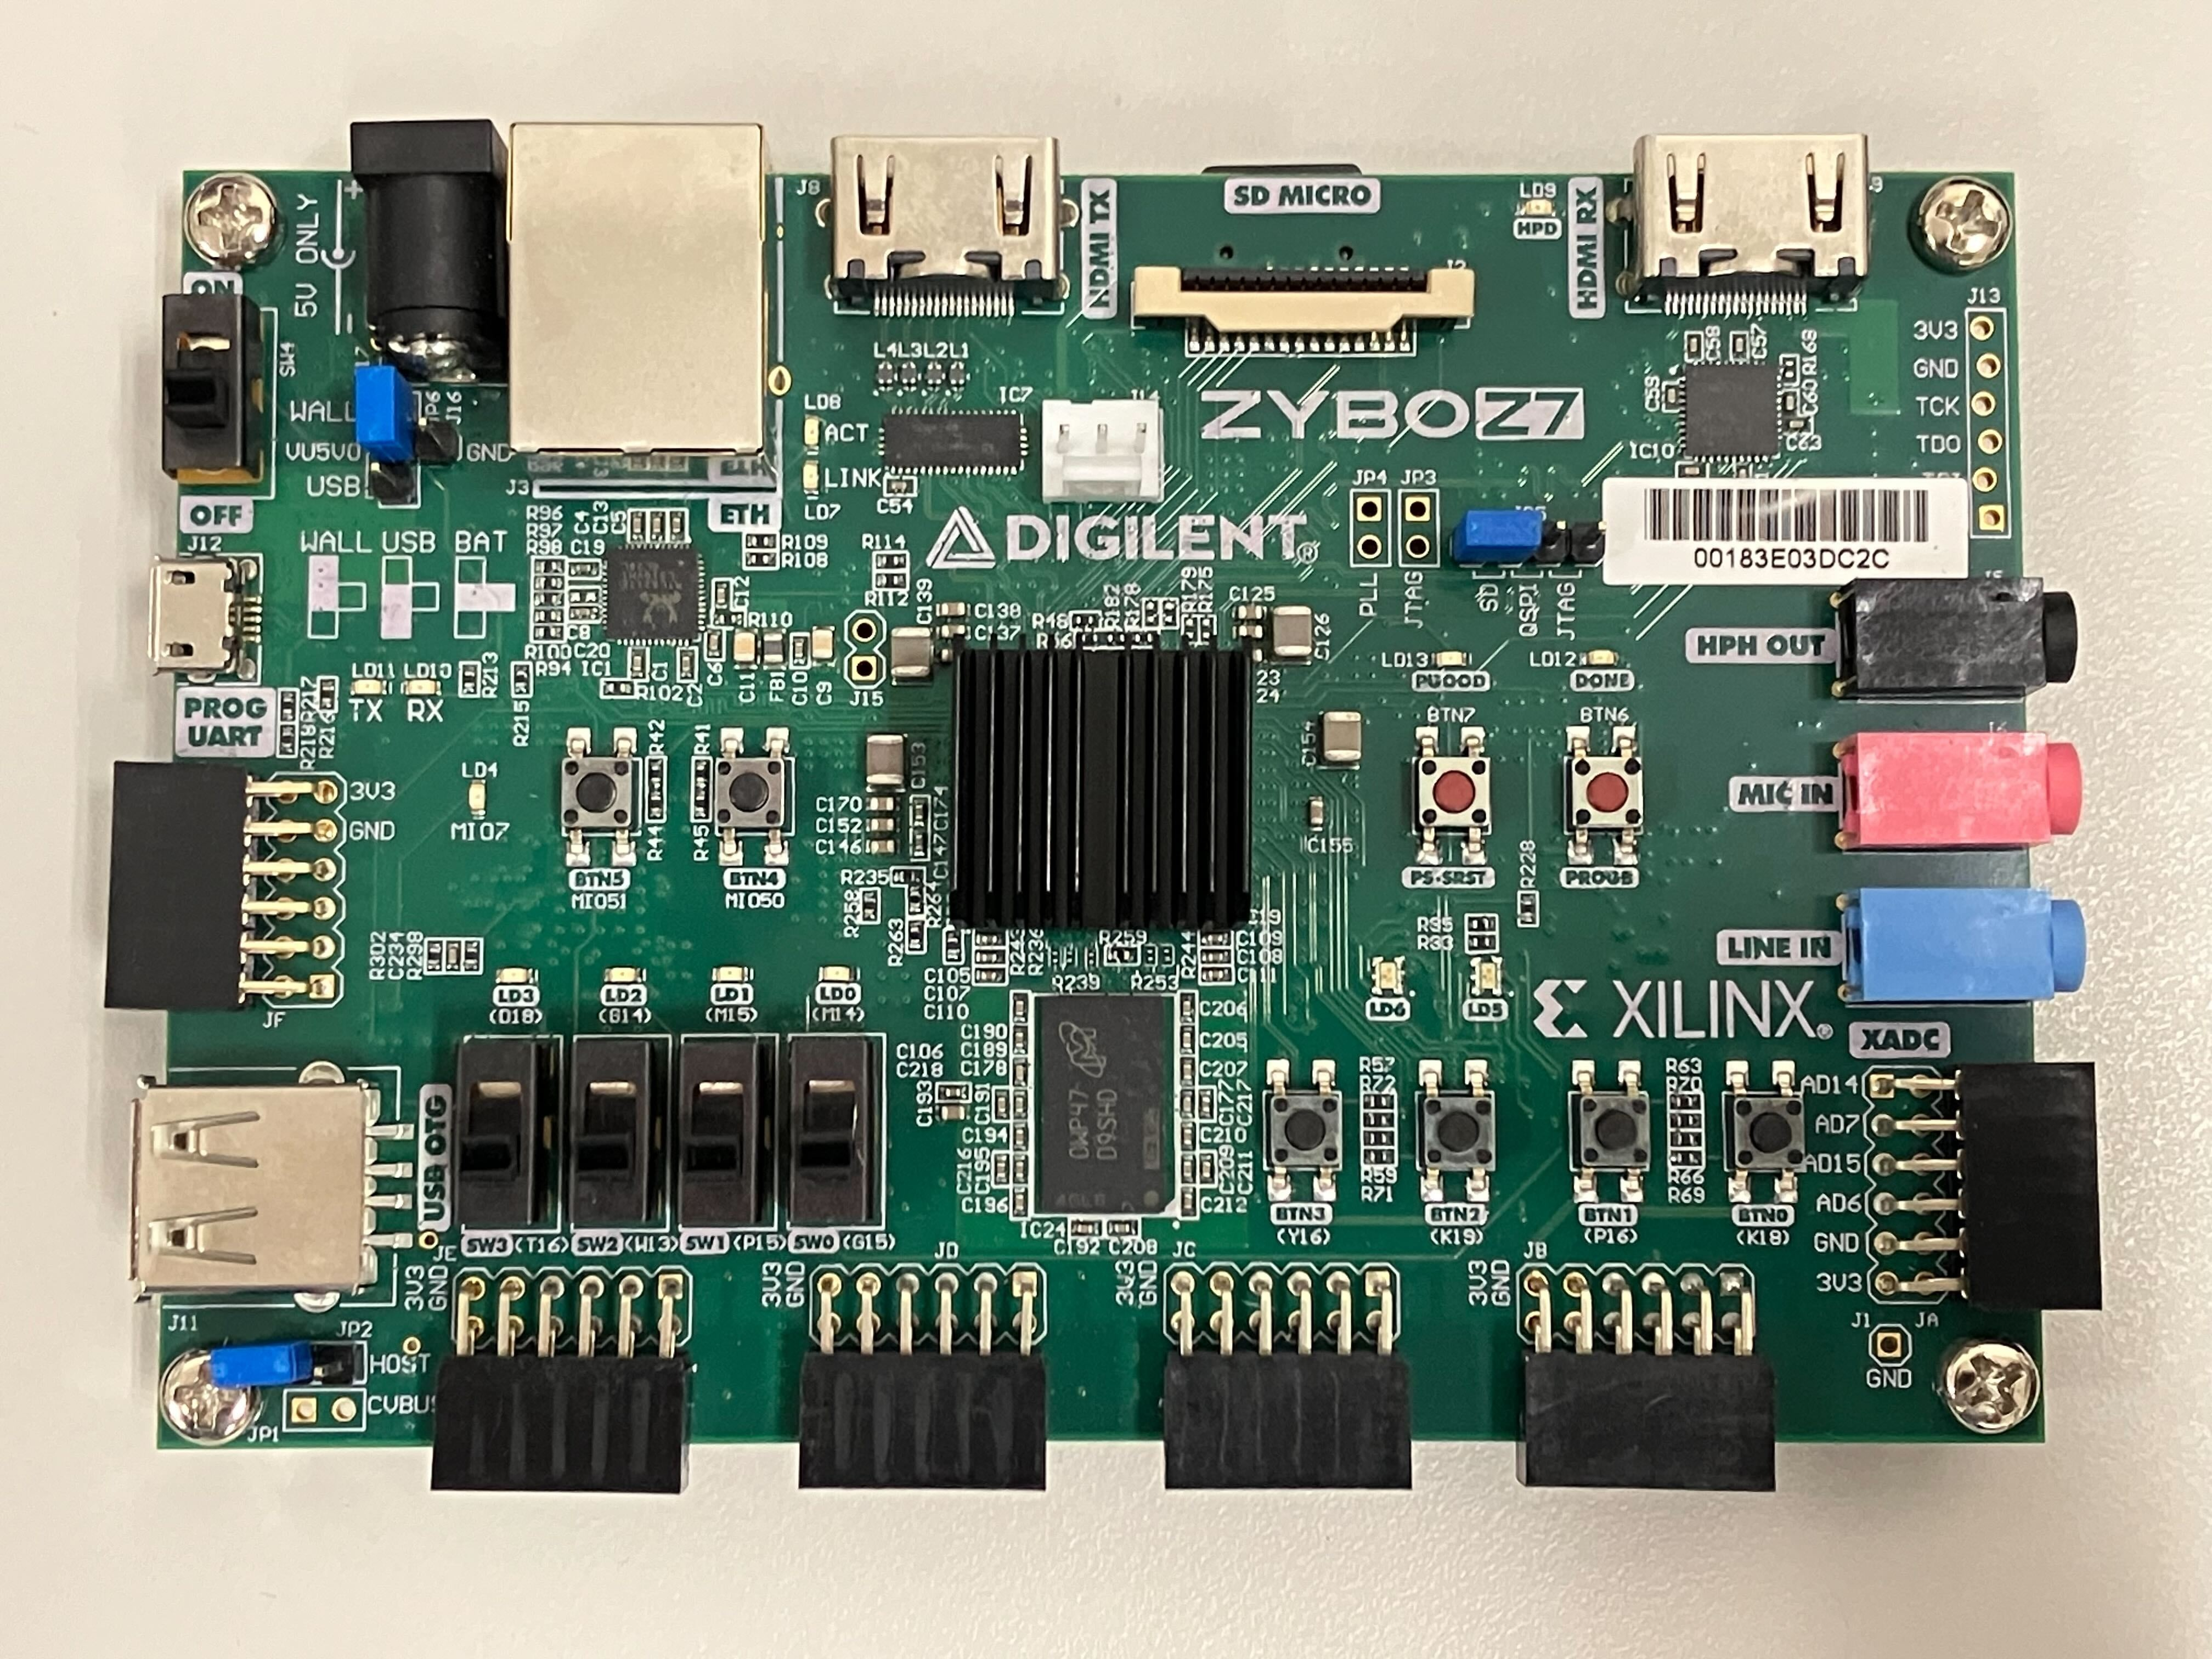
\includegraphics[keepaspectratio, scale=0.045]{4_elDAQ/figs/Zybo.jpg}
      \subcaption{FPGAボードZybo Z7-20 \cite{Zybo}}
    \end{minipage}
    %---- 図はここまで ----------------------
  \end{tabular}
  \vspace{5pt}
  \caption{仰角方向の角度データ読み出し}
  \label{el_daq}
\end{figure}

方位角方向の角度データは、回転台下部に取り付けられたロータリーエンコーダー(HEIDENHAIN, ERM220 \cite{ERM220})を使用し、Xilinx製のFPGAボードSpartan3E \cite{Spartan}で読み出す(図\ref{az_daq})。エンコーダー自体の角度分解能は2.6分角($4.4\cdot {10^{-2}}~^{\circ}$)である。さらに、平滑化フィルターを用いた方位角データの補完を行うことで、角度分解能を$5.7\cdot {10^{-2}}$分角($9.5\cdot {10^{-4}}~^{\circ}$)に向上させている\cite{ikemitsu}。

\begin{figure}[h]
  \begin{tabular}{cc}
    %---- 最初の図 ---------------------------
    \begin{minipage}[t]{0.45\hsize}
      \centering
      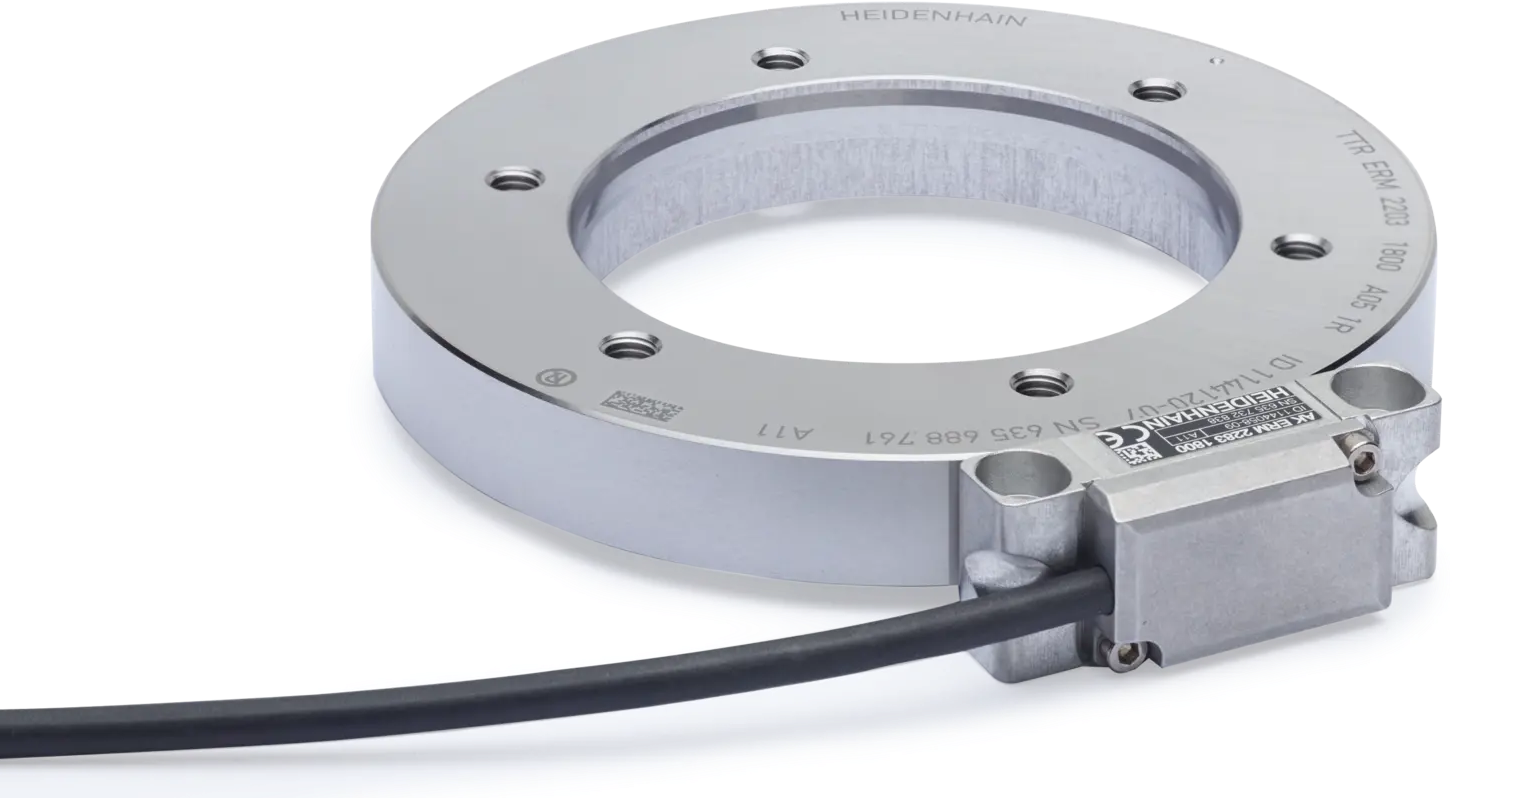
\includegraphics[keepaspectratio, scale=0.1]{4_elDAQ/figs/ERM220.png}
      \subcaption{ロータリーエンコーダー(HEIDENHAIN, ERM220 \cite{ERM220})}
    \end{minipage}
    %---- 2番目の図 --------------------------
    \begin{minipage}[t]{0.45\hsize}
      \centering
      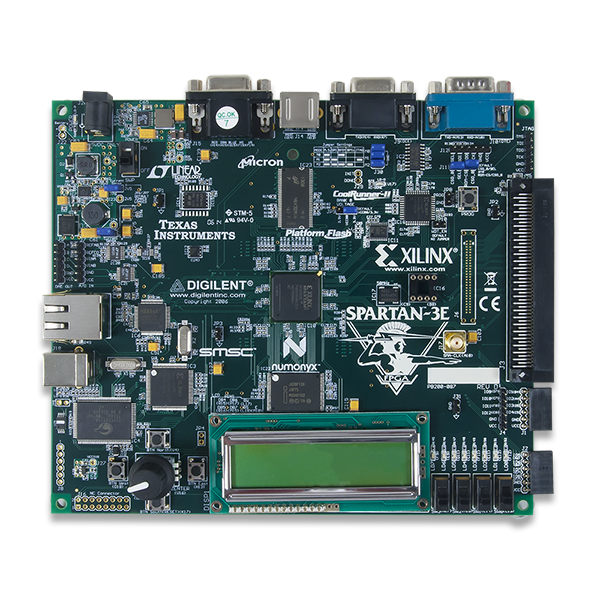
\includegraphics[keepaspectratio, scale=1.1]{4_elDAQ/figs/spartan-3e-2.png}
      \subcaption{FPGAボードSpartan3E \cite{Spartan}}
    \end{minipage}
    %---- 図はここまで ----------------------
  \end{tabular}
  \vspace{5pt}
  \caption{方位角方向の角度データ読み出し}
  \label{az_daq}
\end{figure}

次に検出器のデータと方位角データに求められる同期精度を見積もる。時刻同期の精度を$\Delta t$とする。GroundBIRDの方位角方向の回転速度は最大で$\SI{120}{^{\circ}}$/sになる。方位角方向での角度分解能$\Delta\phi$は
\begin{equation}
  \Delta\phi = \SI{120}{^{\circ}}/\mathrm{s} \cdot \Delta t
\end{equation}
になる。時刻同期による角度の決定精度がエンコーダーの角度分解能よりも十分小さいことを課す。時刻同期による角度決定精度をデータ補完によって向上したエンコーダーの角度分解能である$9.5\cdot {10^{-4}}~^{\circ}$の\SI{1}{\%} 未満と要求すると、$\Delta t$の上限は
\begin{equation}
  \Delta t < \frac{9.5\cdot {10^{-4}}~^{\circ}\cdot 0.01}{\SI{120}{^{\circ}}/\mathrm{s}} = \SI{79}{\mathrm{ns}}
\end{equation}
となる。この正確な時刻同期が必要になるため、仰角と方位角の角度データ読み出しで共にFPGAボードを使用している。先行研究 \cite{ikemitsu}により、時刻同期精度を\SI{55}{ns} に抑え、要求を満たす精度を実現している。

\begin{figure}[htbp]
  \centering
  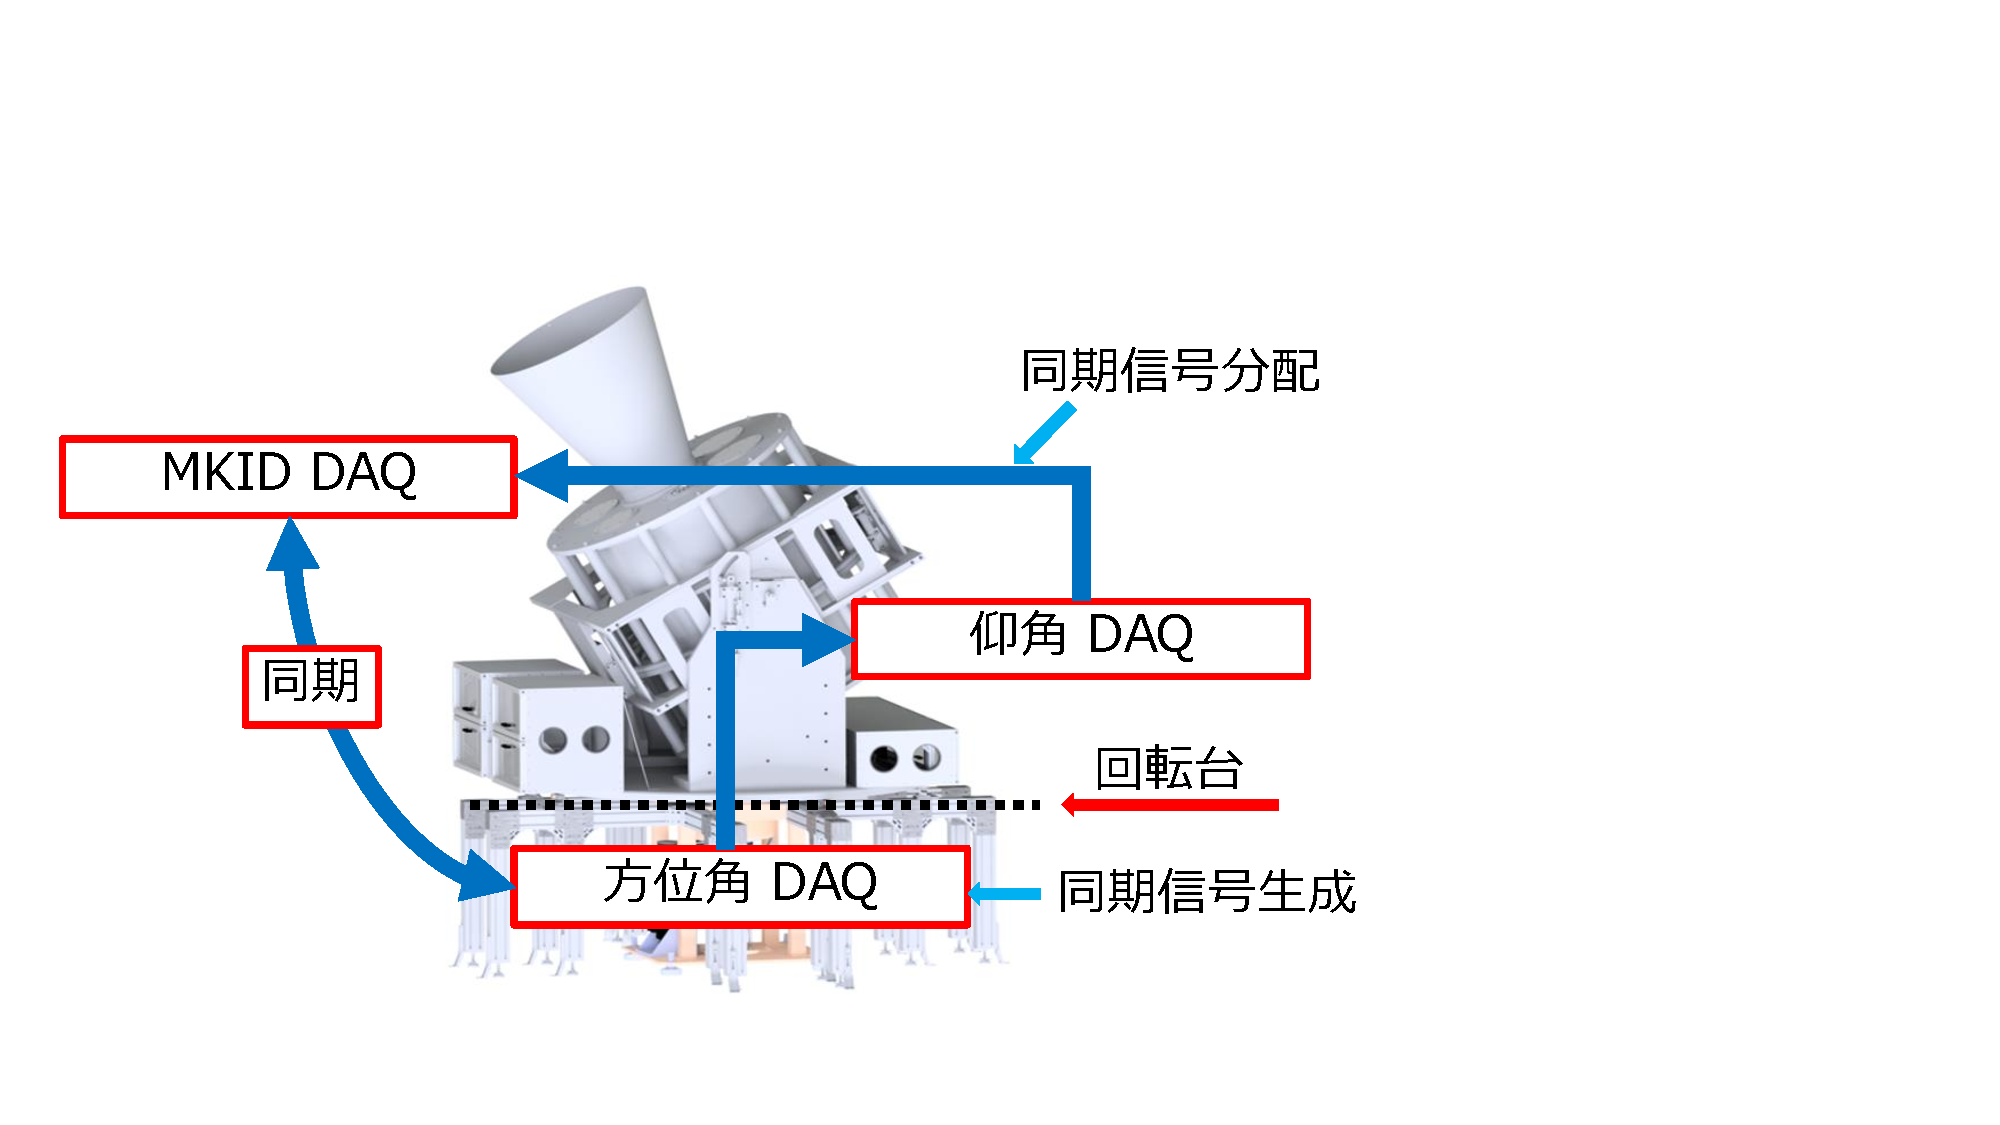
\includegraphics[width=0.9\columnwidth]{4_elDAQ/figs/GB_sync_2.pdf}
  \caption{GroundBIRDの同期信号の流れ。回転台下部の方位角DAQボードで生成された同期信号が回転継手を介して回転台上部のMKIDのDAQボードに送信される。その際、仰角DAQボードで同期信号を分配している。}
  \label{GB_sync}
\end{figure}

GroundBIRDでの同期信号の流れを説明する(図\ref{GB_sync})。望遠鏡が連続回転するため、回転台の上下の電気的な接続に同軸ケーブルのような通常の信号線は使用できない。そのため、回転継手を介して回転台上下での信号を共有している。また、回転台の上下のデータ取得系でレートの遅い``同期信号''を回転継手を介して共有することで時刻の同期を図っている。

同期信号によるデータ同期を次のステップで行なっている。
\begin{enumerate}
  \item 回転台下部の方位角DAQボードから1秒に1回、基準となる同期信号を出力する。
  \item 回転継手を介して回転台上部に届いた同期信号を仰角DAQボードに入力する。
  \item 回転台下部では、同期信号を出力した時刻情報を方位角のエンコーダーデータと共に保存する。
  \item 仰角DAQボード同期信号を分配し、検出器のDAQボードに送る。
  \item 同期信号の到達した時刻情報を検出器のTODと共に保存する。
  \item 2種類のTODの時刻情報を用いて、各時刻での検出器信号と角度データの同期を行う。
\end{enumerate}

\subsection{仰角データ取得における問題点}
本論文の研究対象である仰角のデータ取得に関して詳細に説明する。仰角のデータ取得系が担う役割は以下の2つである。
\begin{itemize}
  \item 仰角の角度データを取得する
  \item 同期信号の分配
\end{itemize}

\begin{figure}[htbp]
  \centering
  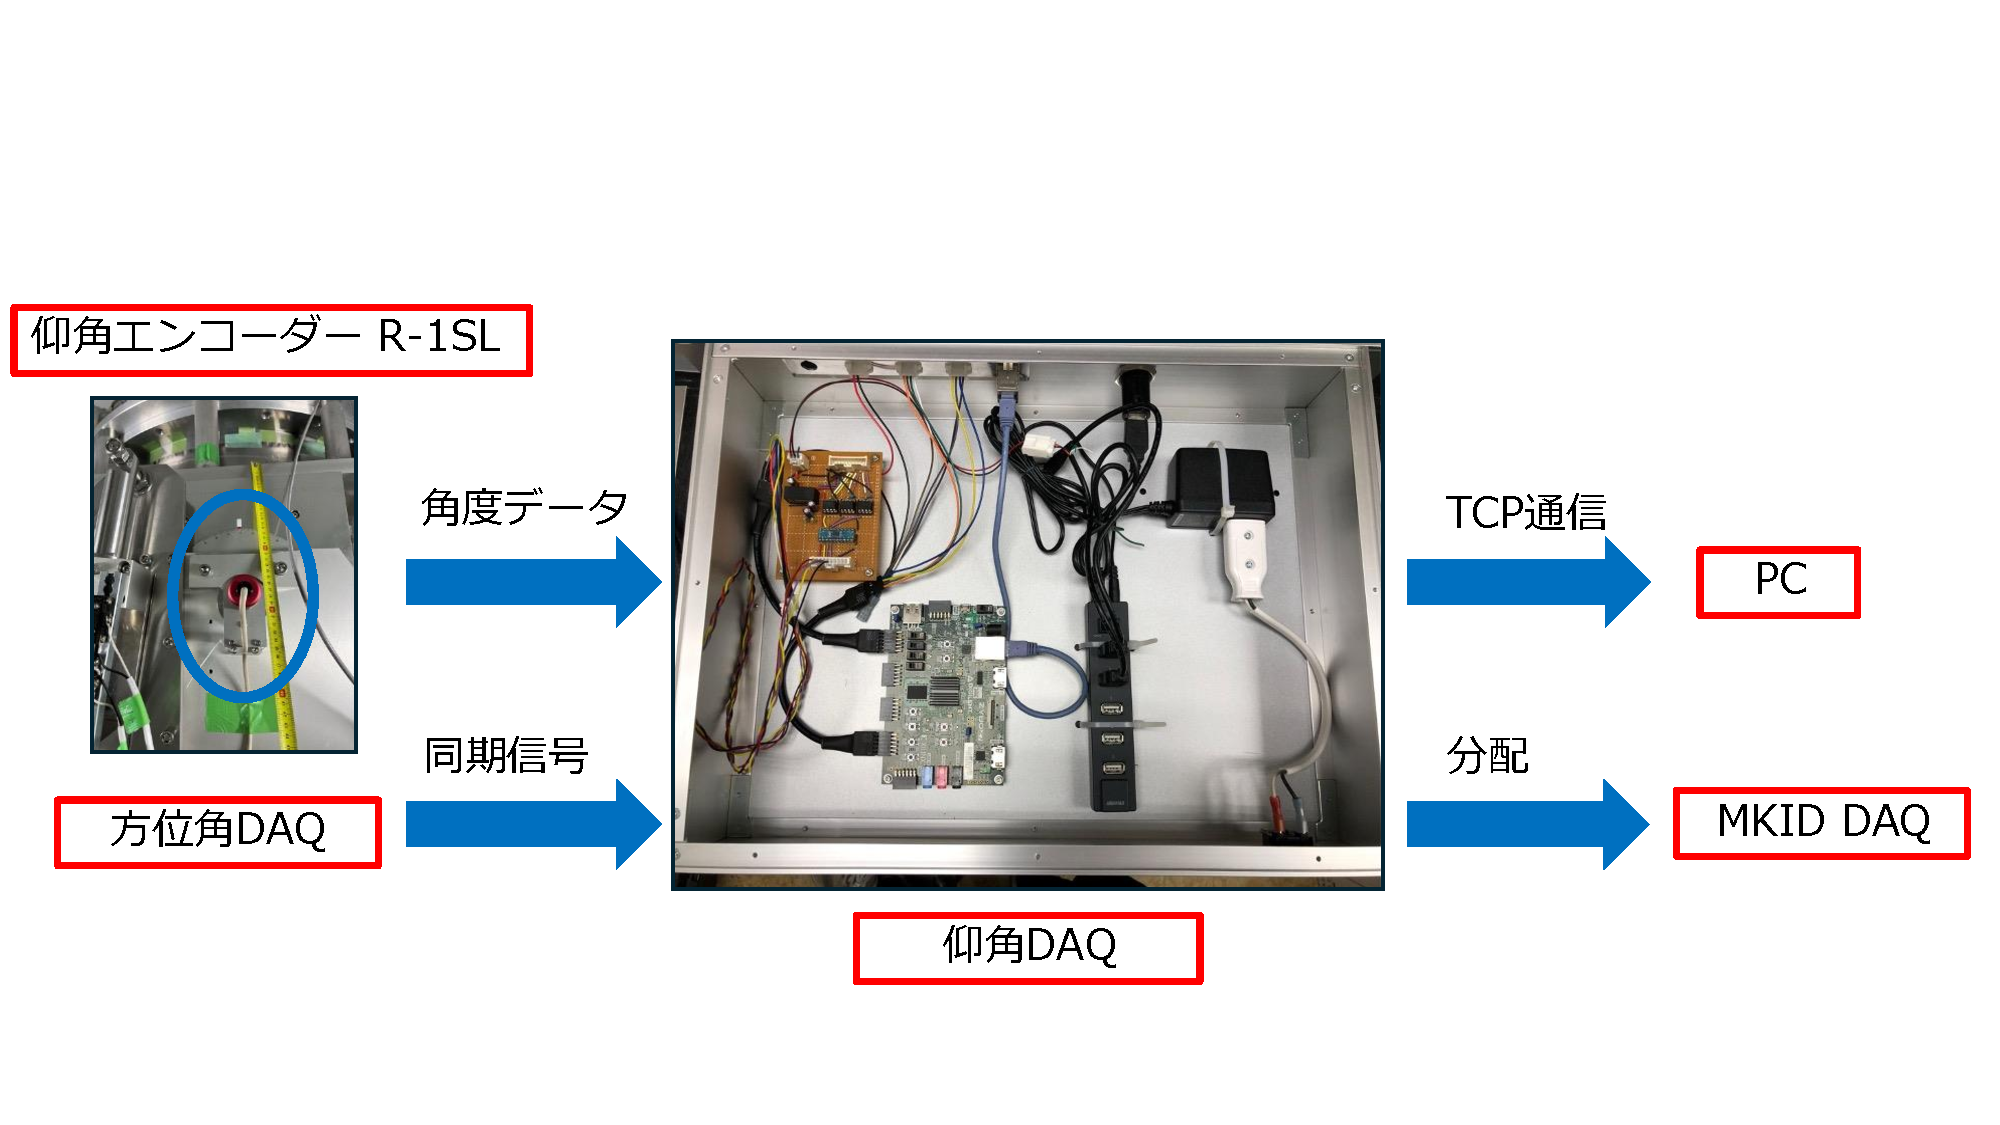
\includegraphics[width=1.0\columnwidth]{4_elDAQ/figs/el_daq_box.pdf}
  \caption{仰角データ取得システムの全体像。信号処理のほぼ全てをZybo \cite{Zybo}が担う。信号の電圧変換、Zybo、電源からなるコンパクトなデータ取得系は1つのボックス内に配置されている。}
  \label{GB_daq_box}
\end{figure}

データ取得系は非常にコンパクトであり(図\ref{GB_daq_box})、信号の処理はZybo内に搭載されている``Zynq \cite{Zynq}''と呼ばれるチップで行っている。ZynqはXilinxが開発した、CPU、FPGAなどが1チップに統合されたSystem on Chip (SoC)の1つである。ZynqはCPUを搭載するProcessing System (PS)部分と、FPGAを搭載するProgrammable Logic (PL)部分に大きく分けられ、FPGAが得意とする並列処理や高速処理と、CPUが得意とする複雑な処理とで役割を分担できるため、効率の良い処理が可能となる。先行研究でFPGAに搭載するファームウェア\footnote{FPGAに組み込む機能を本論文ではファームウェアと呼ぶことにする。}の開発がなされており、実装されている。

\begin{figure}[htbp]
  \centering
  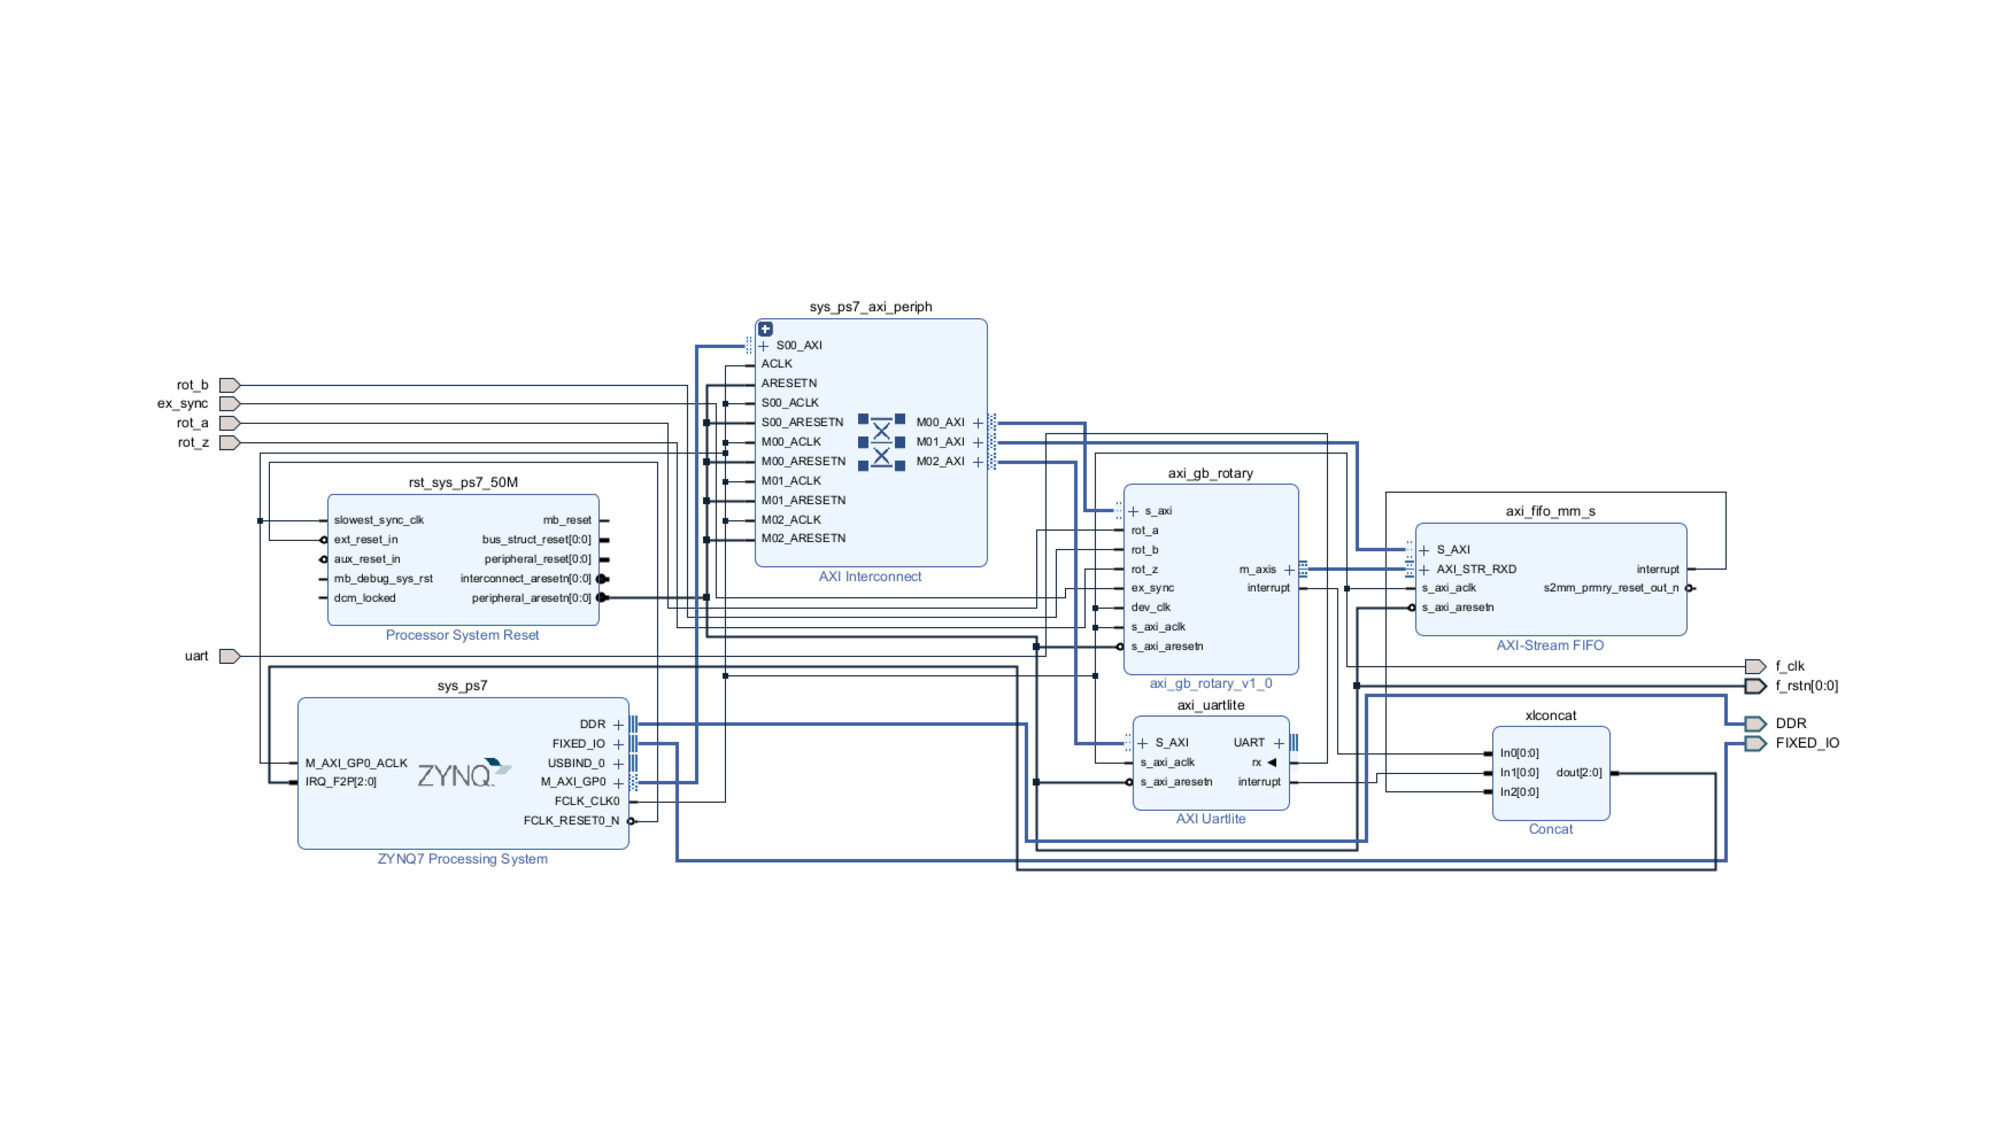
\includegraphics[width=1.0\columnwidth]{4_elDAQ/figs/block_diagram.pdf}
  \caption{IPインテグレータの配線図。青く囲まれているブロックがIPコアを表す。ブロックの左側から出る線が入力信号で、右側から出る線が出力信号になっている。図中の``axi\_gb\_rotary''と呼ばれるIPが自作IPで、デコーダーの役割を担っている。}
  \label{block_diagram}
\end{figure}

FPGA上でのファームウェアの全体図を図\ref{block_diagram}に示す。設計にはVivado\cite{Vivado}というXilinx製の開発ソフトを用いる。様々なIPコア(機能ごとの回路のまとまり)をIPインテグレータというGUI上で配線し、全体のファームウェアを構成する。IPは自作のIPと、Xilinx製のIPを組み合わせて使用している。

\begin{figure}[htbp]
  \centering
  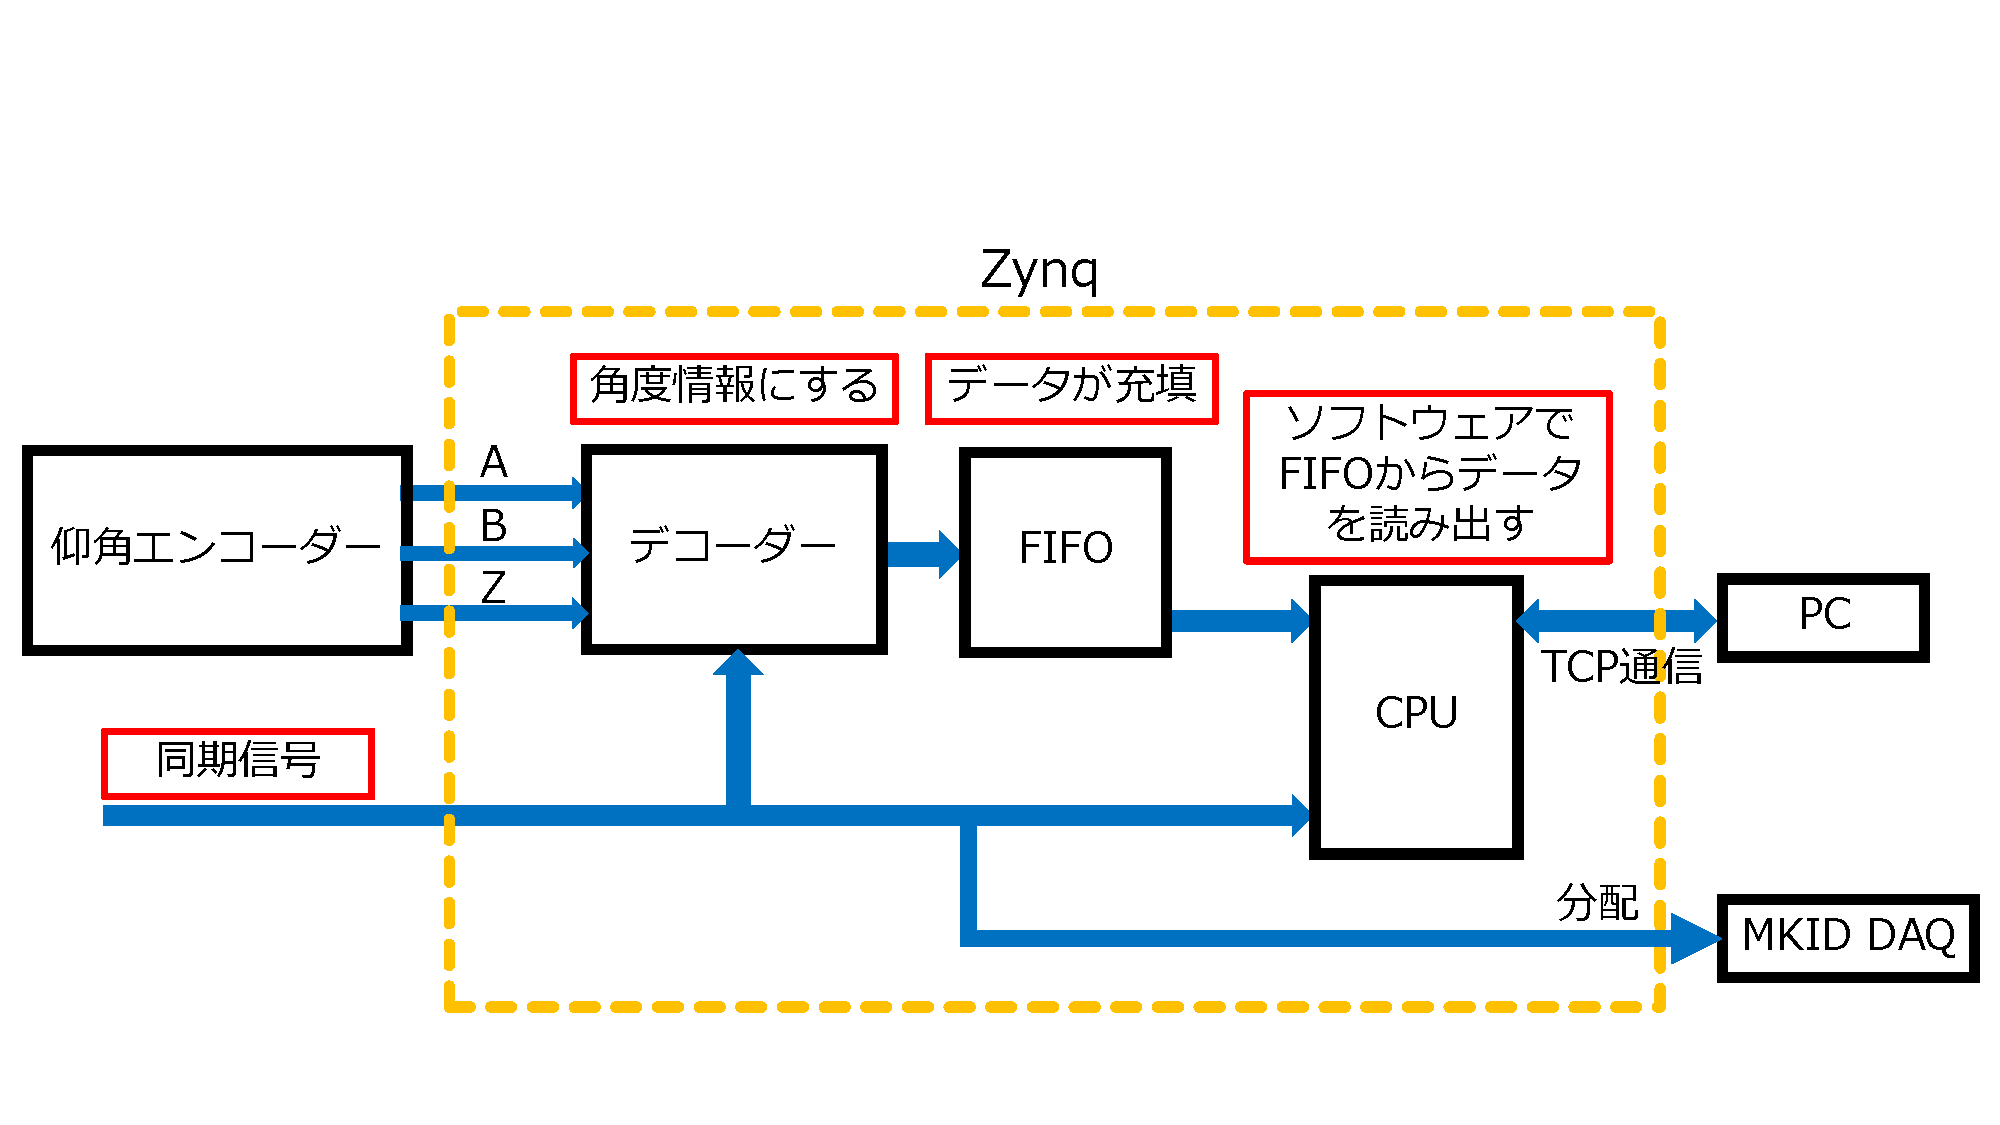
\includegraphics[width=1.0\columnwidth]{4_elDAQ/figs/zynq_flow.pdf}
  \caption{Zynq内での信号処理。エンコーダーからの角度データ処理と方位角DAQボードからの同期信号の分配を1チップ内で行う。}
  \label{zynq_flow}
\end{figure}

Zynq内での処理の模式図を図\ref{zynq_flow}に示す。仰角エンコーダーはインクリメンタル方式を採用しており、エンコーダーからの出力信号は A相、B相、Z相の3相からなる。エンコーダーからの出力パルス数で角度の変化量、A相とB相のパルスの立ち上がり順で回転方向が分かる仕様になっている。また、Z相信号は1回転で1度出力され、回転の原点として使用される。3相の信号はZynq内のデコーダー部分で角度情報として翻訳され、\SI{1}{kSPS}で``FIFO \cite{FIFO}''に充填される。FIFOとはfirst-in first-outメモリのことで、データを格納し、取り出す際は、格納した順番通りに先に格納したデータから取り出す構成になっている。FIFOに格納されたデータはCPUのソフトウェアで読み出し、TCP通信でPCへと送信される。

同期信号の通信方式はUART\footnote{UART通信では、送信側と受信側で通信速度を決めておき、\SI{1}{byte} (\SI{8}{bits})ずつ情報のやり取りを行う。\SI{1}{byte}のまとまりでは、``start bit (\SI{1}{bit})''、``data (\SI{8}{bits})''、``parity bit (\SI{1}{bit}、情報の誤検知に使用)''、``stop bit (\SI{1}{bit})''の4つで構成され、全\SI{11}{bits}になる。}を使用している。デコーダー部分では測定開始時からの経過時間として\SI{1}{kHz}でインクリメントする``タイムスタンプ''を生成しており、同期信号が入力されると同期信号の時間情報を読み取り、このときのタイムスタンプ情報を取得する。タイムスタンプ情報はソフトウェアから読み出す。また、MKIDのDAQは複数のボードを使用するため、同期信号を分配させ、送信している。

\begin{figure}[htbp]
  \centering
  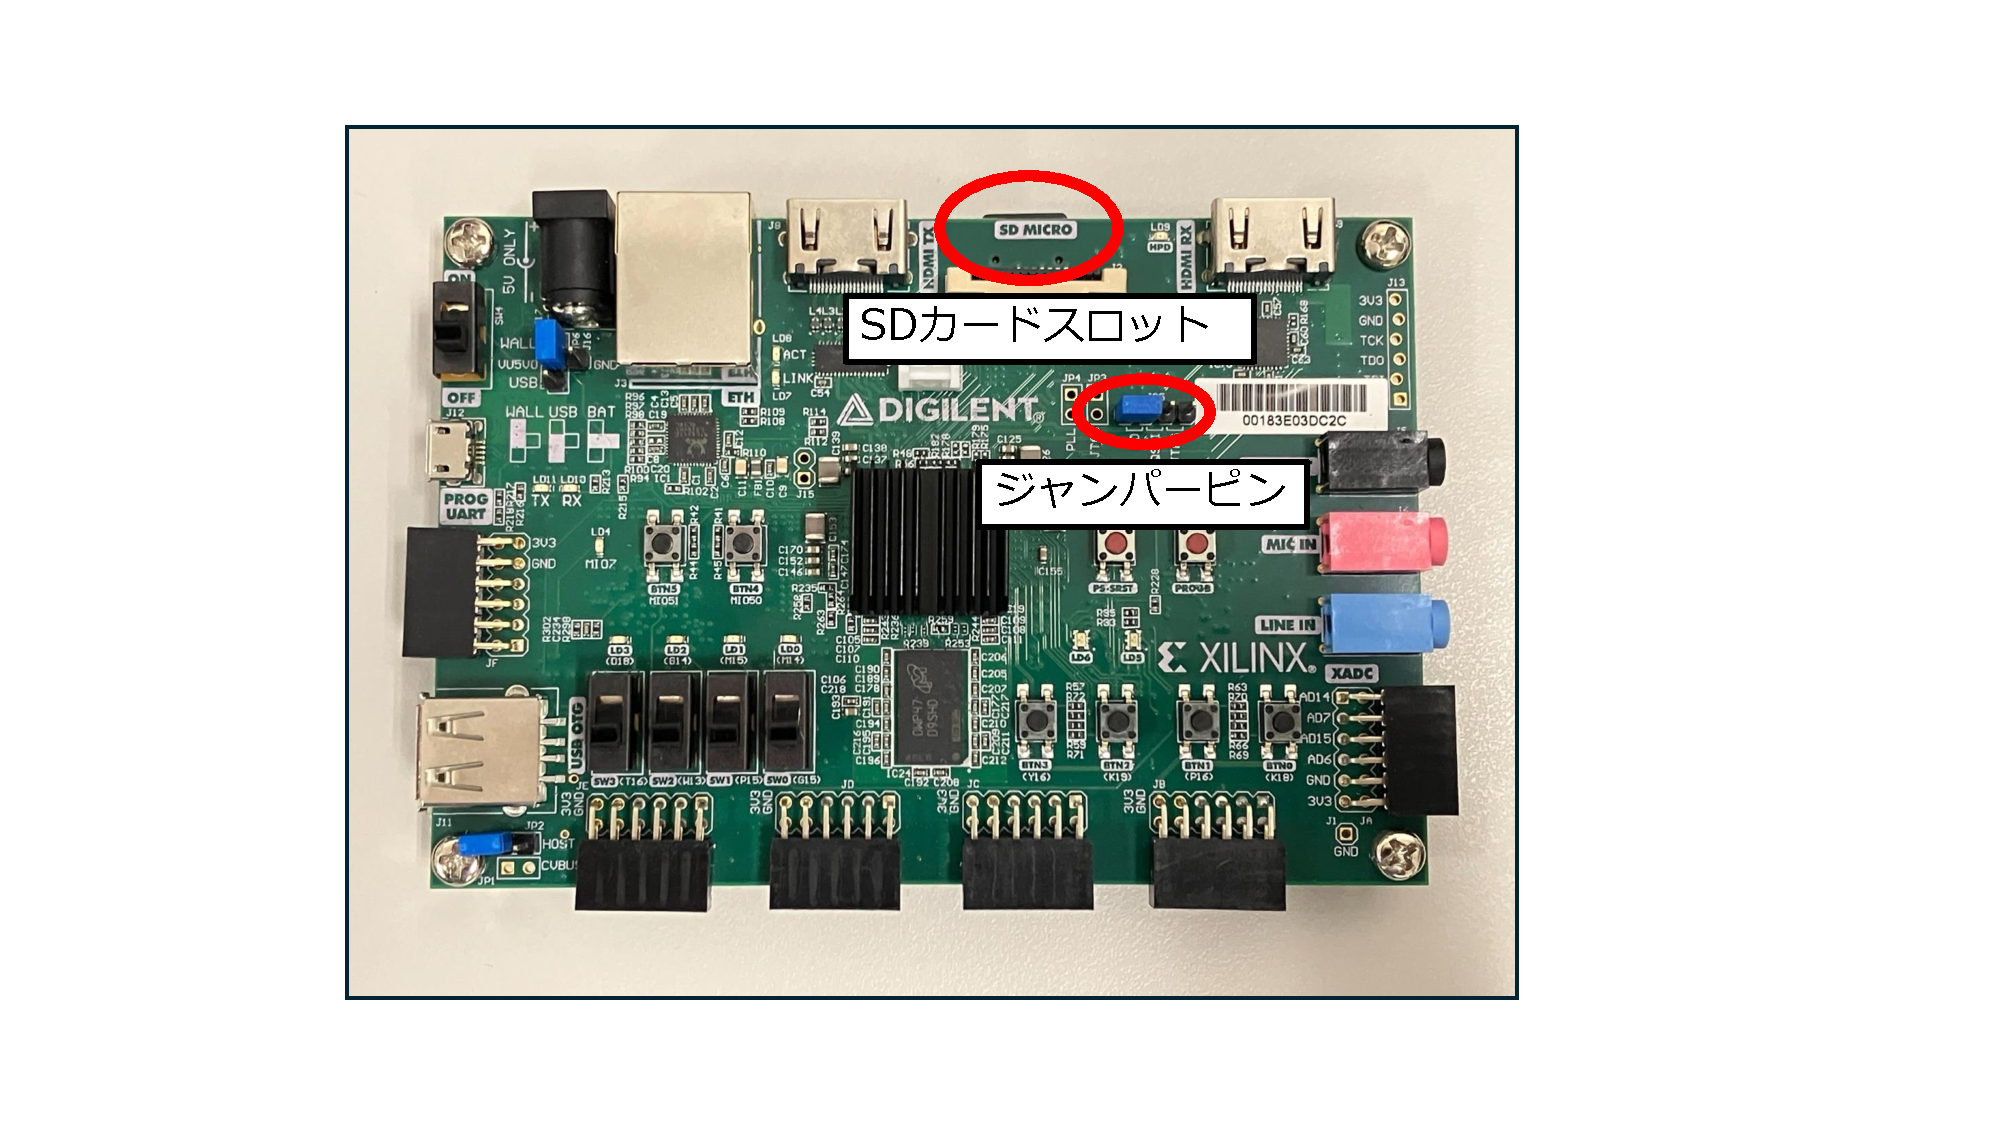
\includegraphics[width=0.6\columnwidth]{4_elDAQ/figs/sd_zybo2.pdf}
  \caption{ZyboにはSDカードスロットが付いている。システムを起動するために必要なファイルをSDカードに書き込み、スロットに差し込んで電源を入れることで稼働が開始する。ジャンパーピンはSDに設定しておく。}
  \label{sd_zybo}
\end{figure}

以上の構成で仰角DAQシステムを稼働させていた(図\ref{sd_zybo})が、観測の長期運用を考えた際に、問題点を抱えていた。Zynqでのデータ処理とPCへの通信をOSのないベアメタル\footnote{本来は「剥き出しの金属」という意味だが、転じてOSがインストールされていないコンピュータのことを指す。}環境でソフトウェアを動かすことで行っている。このことにより、システム全体が硬直的になっており、その扱いにおいて柔軟性がない。柔軟性がないことで起きる問題として以下のものが挙げられる。
\begin{itemize}
  \item データ取得が異常終了した際のメンテナンスが難しい
  \item OSが介さない通信による信頼性の低下
  \item ソフトウェア、FPGA面での改良が難しい
\end{itemize}

最も大きな問題はメンテナンス性である。観測の有無に問わず、望遠鏡の角度データは常に取得し続けており、安定した仰角データ取得が必要不可欠である。しかし、仰角エンコーダーからPCまでのデータの流れが途切れてしまうことがある。それは、通信のエラーや停電等による電源系統の不具合など様々な要因からくるもので、長期運用をする上ではある程度避けられないものである。その際、エンコーダーとZybo間の通信が切れて、Zynq内でのエンコーダー情報が失われる。加えて、エンコーダーの原点情報も失われるため、通信を再開させた際に読み出した角度の値にオフセット値が乗ってしまう。Zynq内で原点情報を記憶させるには望遠鏡の仰角を動かし、エンコーダーのZ相信号を取得して値をリセットすることが必要であり、手間のかかる工程になる。この一連のメンテナンスをまとめると以下のステップに分けられる。
\begin{enumerate}
  \item Zyboを再起動させて再度ソフトウェアを動かす
  \item 望遠鏡の仰角を動かしてZ相信号を入力し、原点情報を記憶
  \item 仰角を$\SI{70}{^{\circ}}$まで動かして固定
\end{enumerate}

この中で、Zyboの再起動と仰角を動かす際にケーブルに変な張力がかかっていないかの目視に現地での作業を要する。リモートでの望遠鏡運用を進める上で、少しでも現地で必要な作業を減らし、リモートでメンテナンスができることが望まれる。

また、ZyboとPCとのTCP通信を行うために、ベアメタル環境ではTCP/IPのプロトコルスタックを独自で実装しなければいけない。今回は``lwIP(lightweight IP)''と呼ばれるオープンソースのTCP/IPプロトコルスタックを使用してTCP通信を実装している。そのため、通信に関わるソフトウェアが複雑化する上、OSが通信を取り仕切るよりも信頼性に欠ける。

加えて、システムに組み込まれたソフトウェアやFPGAのファームウェアは固定化されており、今後の運用で変更点が生じた時に、SDカードに新しいファイルシステムを書き込んで全面的にシステム更新しなければならず、労力を要する。システムのカスタマイズ性を上げ、変更を容易にできるようになれば、運用に関わるコストを削減することができる。

\subsection{PYNQを用いた新システムの導入}
上に述べた問題を改善するために、本研究では既存のZynqシステムにOSを搭載し、ソフトウェアをOS上で動かすことでシステム全体の柔軟性向上を試みた。これにより上記の問題点に対して
\begin{itemize}
  \item データ取得が異常終了した際のメンテナンスをリモート主体で行える
  \item OSが通信を介すことで信頼性が向上
  \item ソフトウェア、FPGA面での改良をシステムを起動したまま行える
\end{itemize}
という改善が期待できる。一方でベアメタル環境に比べてOSをインストールすることで実行時間と使用メモリが増えるが、FIFOへのデータ充填とFIFOからの読み出しはともに\SI{1}{kSPS}であり、FIFOの容量も十分であるため、性能に問題は出ない。Zynqに搭載するOSは基本的にlinuxベースであるが、今回は``PYNQ \cite{Pynq}''と呼ばれるUbuntu\footnote{今回はUbuntu 22.04がベースになっている}、JupyterおよびPythonをベースとしたフレームワークを搭載した。PYNQを採用した理由として
\begin{itemize}
  \item ソフトウェアをPYNQ上のPythonスクリプトで動かせるため、通信スクリプトを簡潔に記述できる
  \item システム起動に必要なブートイメージファイルの作成が容易
  \item ``Overlay''と呼ばれる機能を使用することでFPGAのファームウェアをPythonで容易に変更できる
\end{itemize}
が挙げられる。

\subsection{PYNQイメージファイルの作成}

%ここでPYNQのイメージファイル作成の概要を説明する。
PYNQのイメージファイルを作成するにあたって、基本的な手順は\cite{image}を参考にし、作業環境はDocker上のUbuntu 20.04で構築した。その際に使用した開発ツールとバージョンを表\ref{PYNQ_table}にまとめる

\begin{table}[htbp]
  \centering
  \caption{PYNQイメージ作成で使用したツールとバージョン}
  \vspace{3mm}
  \begin{tabular}{cc} \hline\hline
    ツール & バージョン \\ \hline
    Vivado & 2022.1\\
    PYNQ linuxイメージ & 3.0.1\\
    PetaLinux & 2022.1\\ \hline\hline
  \end{tabular}
  \label{PYNQ_table}
\end{table}

PetaLinuxとはXilinxが提供する、ZynqをはじめとするSoC用のlinuxシステムをビルドするためのツールである。この環境のもとで以下のステップでPYNQイメージを作成した。
\begin{enumerate}
  \item ベースとなるFPGAファームウェアの作成

  FPGAファームウェアはOverlayによってZybo起動時に変更できるため、この時点では最も単純な回路をVivadoで準備してやれば良い。それをもとにVivado上でコンパイルをし、生成された4つの回路情報を持つファイル(.xsaファイル、.bitファイル、.hwhファイル、.tclファイル)を取得する。
  \item Zybo用のスペックファイルの作成

  スペックファイルはZyboのスペック情報を.specファイルとして作成する。その後、作成した全ファイルをビルド用のディレクトリに置く。
  \item ビルド

  最後にmakeを実行してビルドを行い、PYNQイメージファイル(.imgファイル)を生成して完了する。
  \item イメージファイルの書き込みとPYNQ起動

  作成したイメージファイルをSDカードにddコマンド等で書き込み、ZyboのSDカードスロットに差し込むことでPYNQが起動する。また、起動時にOverlayスクリプトを走らせて図\ref{block_diagram}で示したファームウェアでFPGAの回路を上書きするように設定した。これにより、本来の回路情報がPYNQ上で再現される。

\end{enumerate}

%FPGAファームウェアはOverlayによってZybo起動時に変更できるため、この時点では最も単純な回路をVivadoで準備してやれば良い。それをもとにVivado上でコンパイルをし、生成された4つの回路情報を持つファイル(.xsaファイル、.bitファイル、.hwhファイル、.tclファイル)を取得する。

%スペックファイルはZyboのスペック情報を.specファイルとして作成する。その後、作成した全ファイルをビルド用のディレクトリに置く。最後にmakeを実行してビルドを行い、PYNQイメージファイル(.imgファイル)を生成して完了する。

%このイメージファイルをSDカードにddコマンド等で書き込み、ZyboのSDカードスロットに差し込むことでPYNQが起動する。また、起動時にOverlayスクリプトを走らせて図\ref{block_diagram}で示したファームウェアでFPGAの回路を上書きするように設定した。これにより、本来の回路情報がPYNQ上で再現される。

Overlayを用いてFPGAのファームウェアを変更する仕組みを図\ref{overlay}に示す。

\begin{figure}[htbp]
  \centering
  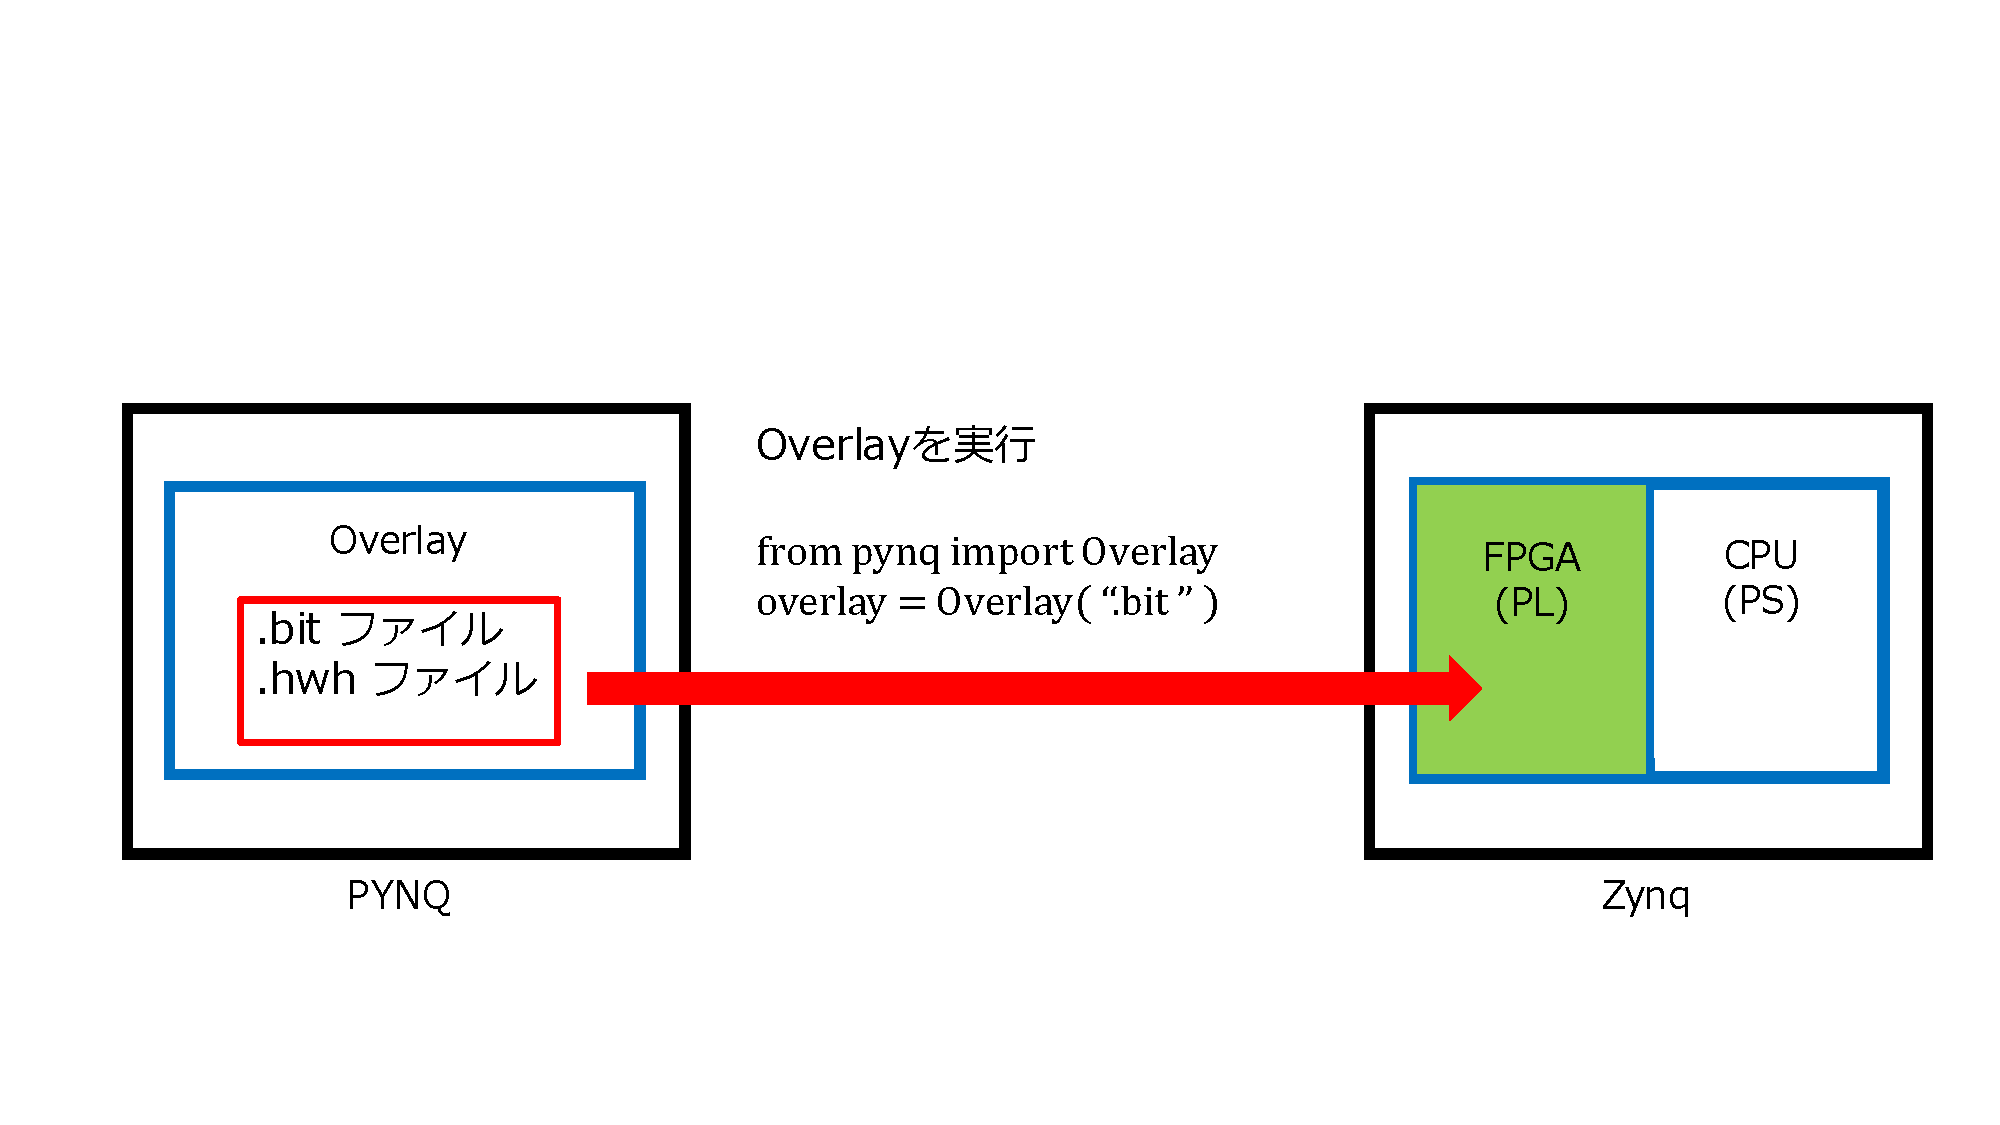
\includegraphics[width=1.0\columnwidth]{4_elDAQ/figs/overlay3.pdf}
  \caption{PYNQからFPGAのファームウェアを変更する模式図。Vivadoで設計した新しい回路ファイルをOverlayクラスに読み込ませることで容易に変更ができる。}
  \label{overlay}
\end{figure}
Overlayに必要なファイルはVivadoでコンパイルをして生成される.bitファイルと.hwhファイルの2つである。これらは同じディレクトリに置いておく。PythonでOverlayクラスをインポートし、.bitファイルを読み込ませることでOverlayは実行される。その際、Overlayクラスは同じディレクトリにある.hwhファイルも読み込んでくれる。図で示したようにOverlayスクリプトはたった2行で書くことができ、ファームウェアの変更は非常に容易に実行できる。

最後に、Zynq内で動かすスクリプトをPYNQ用にPythonで再構築した。

\section{望遠鏡への実装}

\subsection{新データ取得システムのインストール}
新しく導入した仰角データ取得システムを、自分の手元でできる動作確認をした後に実際の望遠鏡に実装、という流れでインストールした。

\begin{figure}[h]
  \begin{tabular}{cc}
    %---- 最初の図 ---------------------------
    \begin{minipage}[t]{0.45\hsize}
      \centering
      \includegraphics[keepaspectratio, scale=0.035]{4_elDAQ/figs/test_pic.jpg}
      \subcaption{動作確認のセットアップ}
    \end{minipage}
    %---- 2番目の図 --------------------------
    \begin{minipage}[t]{0.45\hsize}
      \centering
      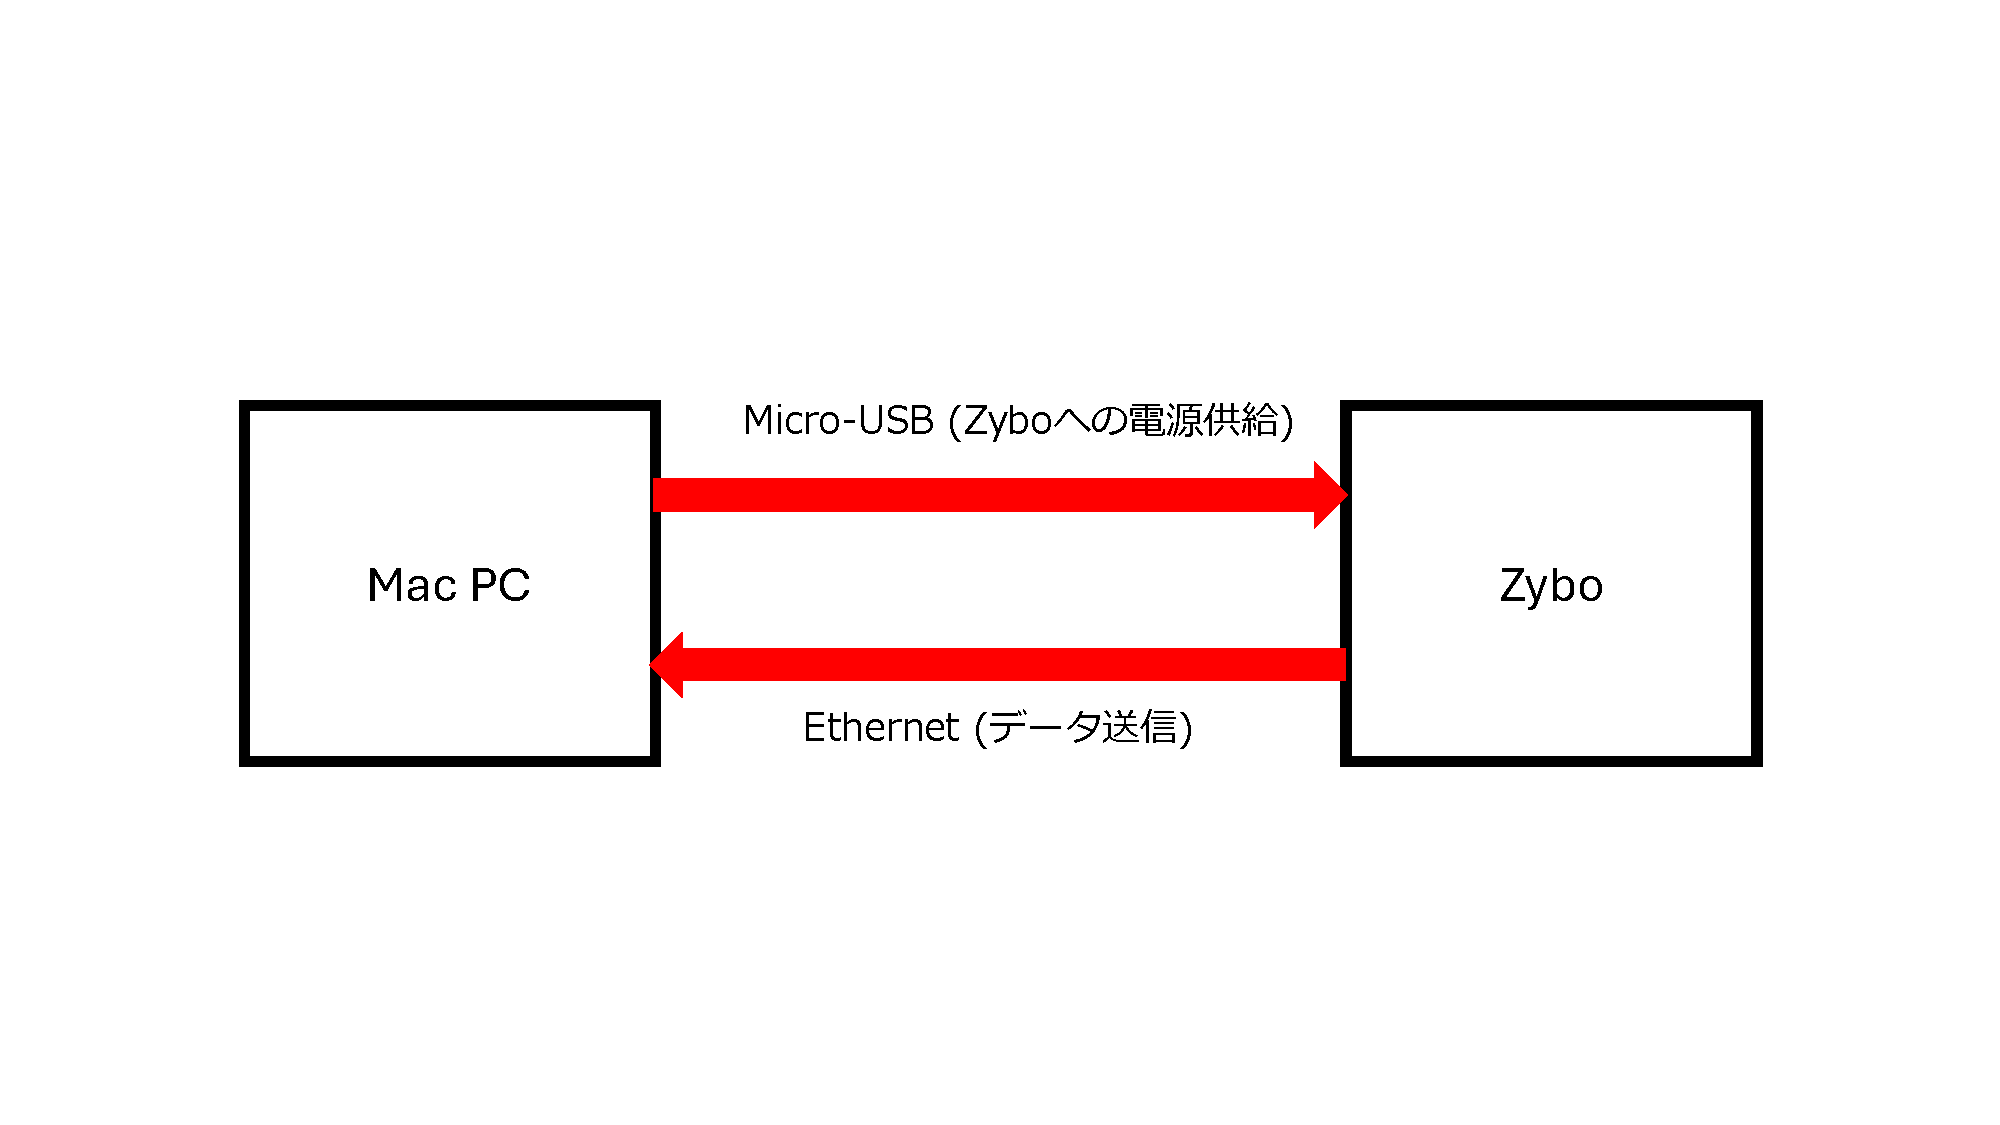
\includegraphics[keepaspectratio, scale=0.35]{4_elDAQ/figs/el_test2.pdf}
      \subcaption{セットアップの模式図}
    \end{minipage}
    %---- 図はここまで ----------------------
  \end{tabular}
  \vspace{5pt}
  \caption{新システムでの動作確認}
  \label{el_test}
\end{figure}

動作確認を、図\ref{el_test}に示したセットアップで行なった。ロータリーエンコーダーとは接続せず、同期信号も送らない単純なものである。図\ref{el_test}の左図にあるように、Zyboの電源を入れPYNQが起動するとボード右側の``DONE''ランプが緑色に点灯する。自分のMac PCをデータ取得PCとして、Micro-USBでZyboへの電源供給を行い、データ通信はEthernetケーブルで行った。PC上でデータ読み出しのスクリプトを動かして、Zynqの挙動に問題がないかをチェックした。期待される挙動は
\begin{itemize}
  \item Zynqが正しく機能し、PC側でデータを読み出せる
  \item エンコーダーデータは0として取得されている
  \item タイムスタンプは時間とともに加算されている
\end{itemize}
の3点である。データの通信が始まるとZyboのEthernetコネクタ付近のランプが点滅し、PC側でのデータ読み出しが正常に動くことを確認した。PCに保存したデータファイルをチェックし、期待されるデータを取得できていることも確認した。取得したエンコーダーデータとタイムスタンプデータのプロットを図\ref{eldata_check}に示す。プロットの横軸はデータのサンプリングナンバー(\SI{1}{kSPS})を表す。

\begin{figure}[h]
  \begin{tabular}{cc}
    %---- 最初の図 ---------------------------
    \begin{minipage}[t]{0.45\hsize}
      \centering
      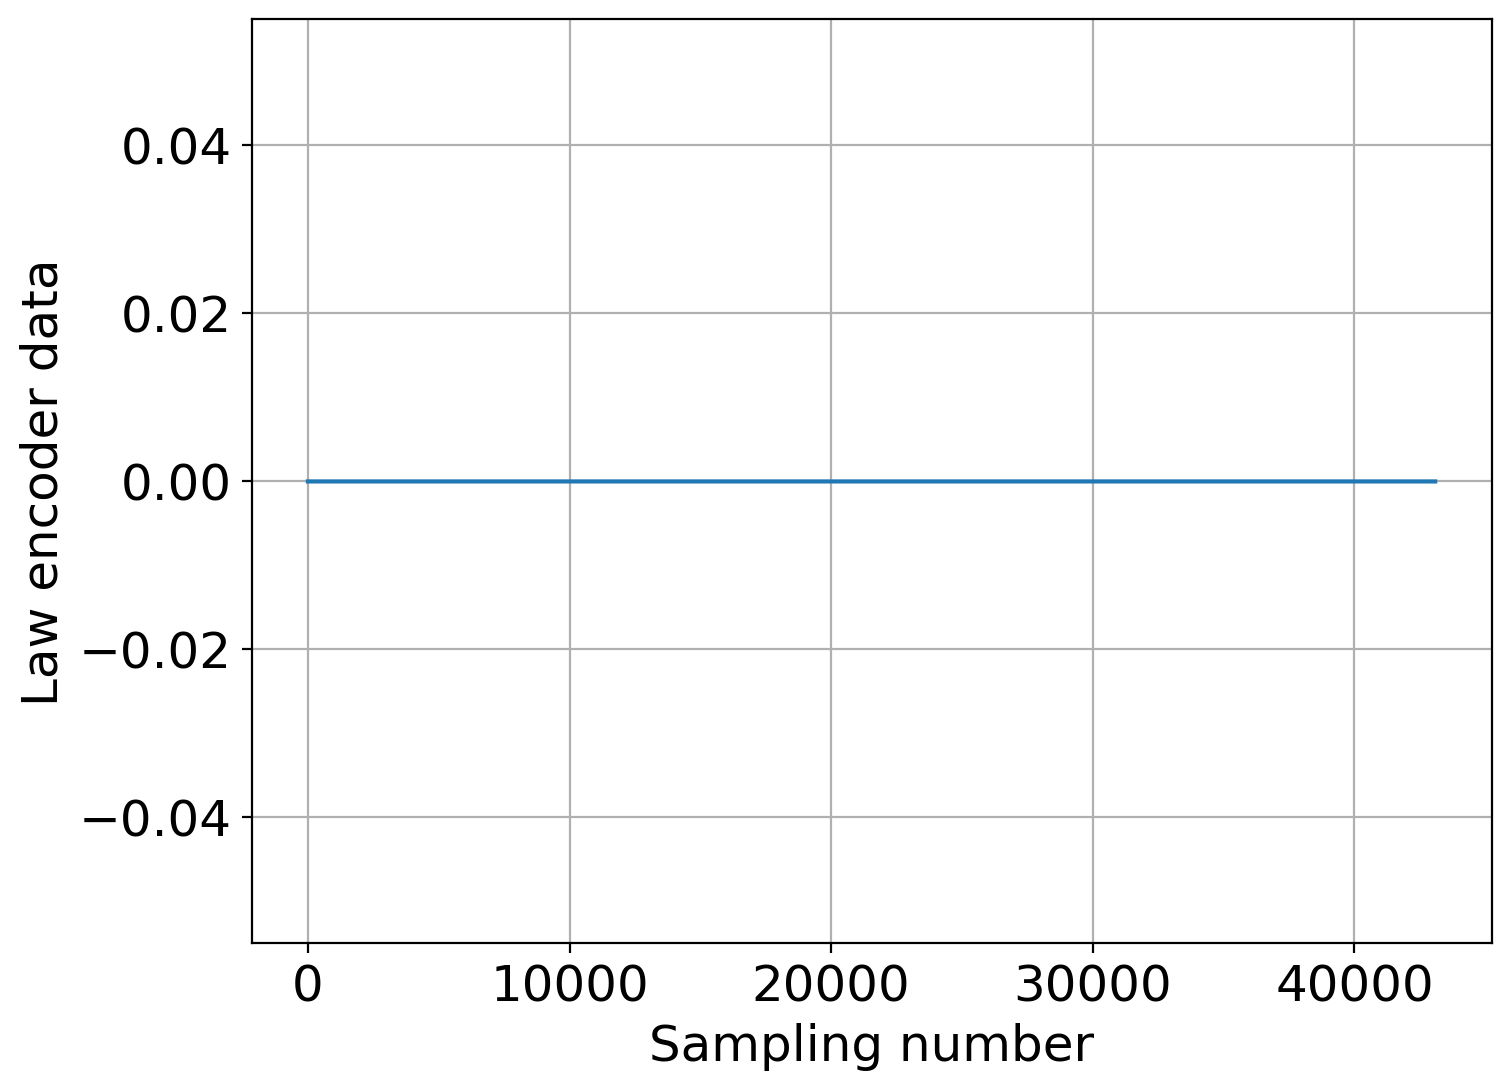
\includegraphics[keepaspectratio, scale=0.35]{4_elDAQ/figs/enc_data_test.png}
      \subcaption{エンコーダーデータ}
    \end{minipage}
    %---- 2番目の図 --------------------------
    \begin{minipage}[t]{0.45\hsize}
      \centering
      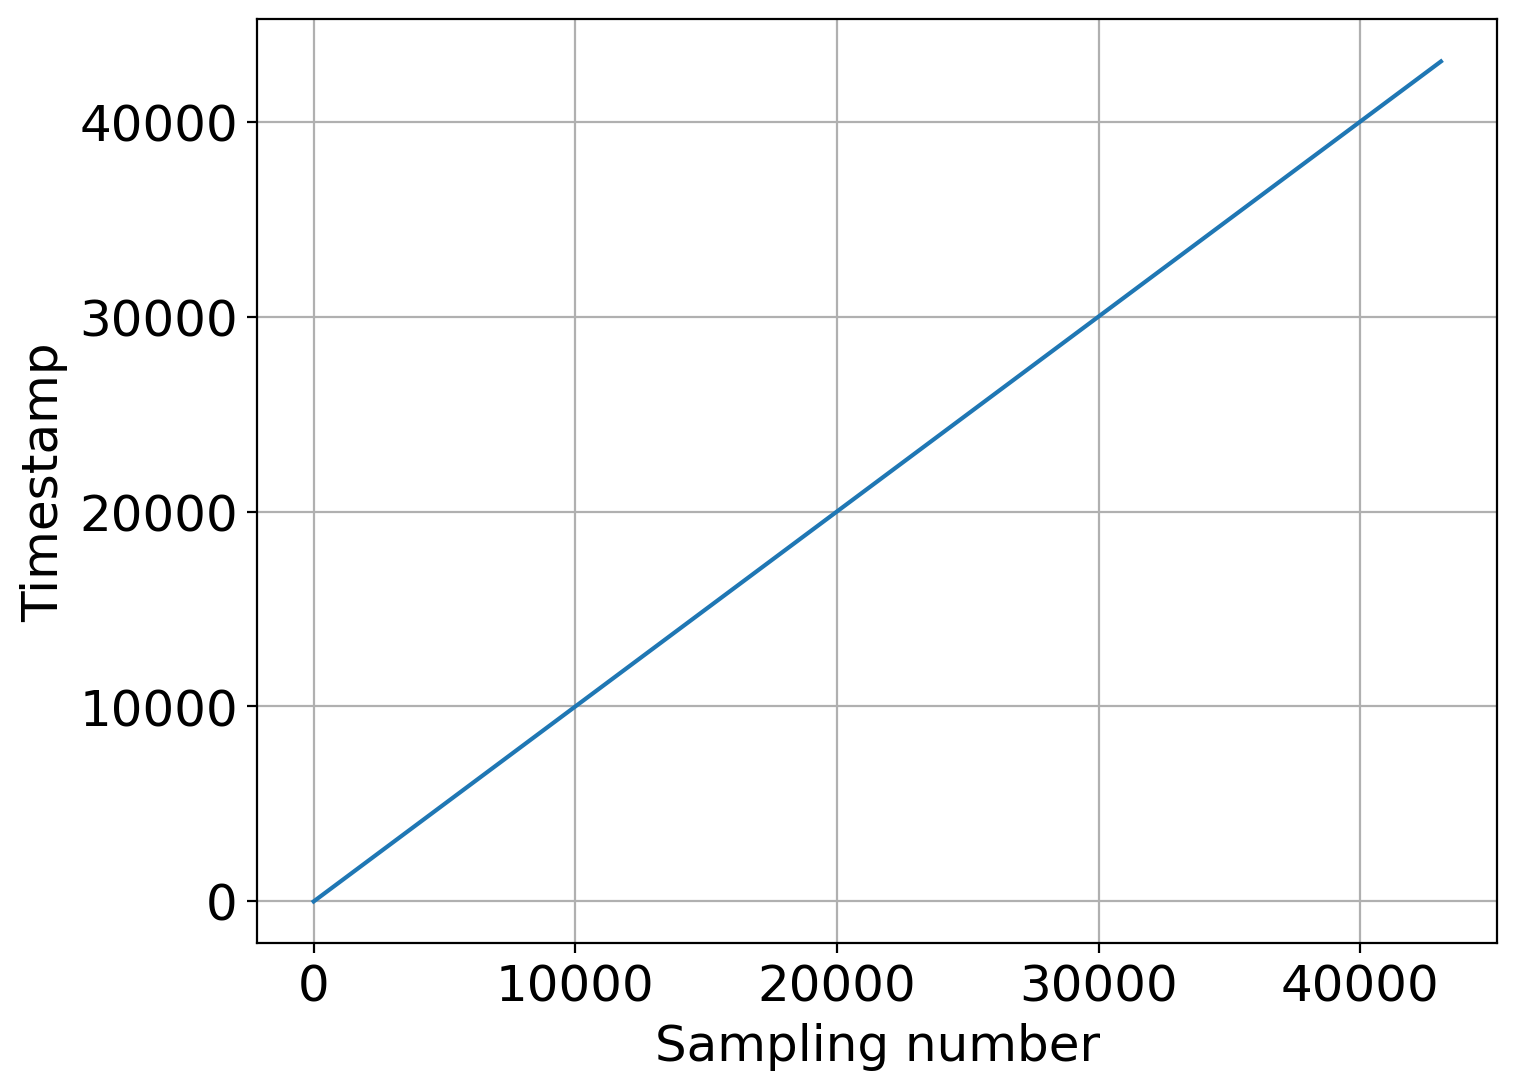
\includegraphics[keepaspectratio, scale=0.35]{4_elDAQ/figs/timestamp.png}
      \subcaption{タイムスタンプ}
    \end{minipage}
    %---- 図はここまで ----------------------
  \end{tabular}
  \vspace{5pt}
  \caption{動作確認で取得したデータ}
  \label{eldata_check}
\end{figure}

以上の結果から、期待される3点の挙動を確認することができたため、新システムに問題はないと判断した。次に実際の望遠鏡へのインストールを行なった。インストールはSDカードを新システムのものに交換するだけで完了し、PYNQの起動を確認した(図\ref{el_install})。

\begin{figure}[h]
  \begin{tabular}{cc}
    %---- 最初の図 ---------------------------
    \begin{minipage}[t]{0.45\hsize}
      \centering
      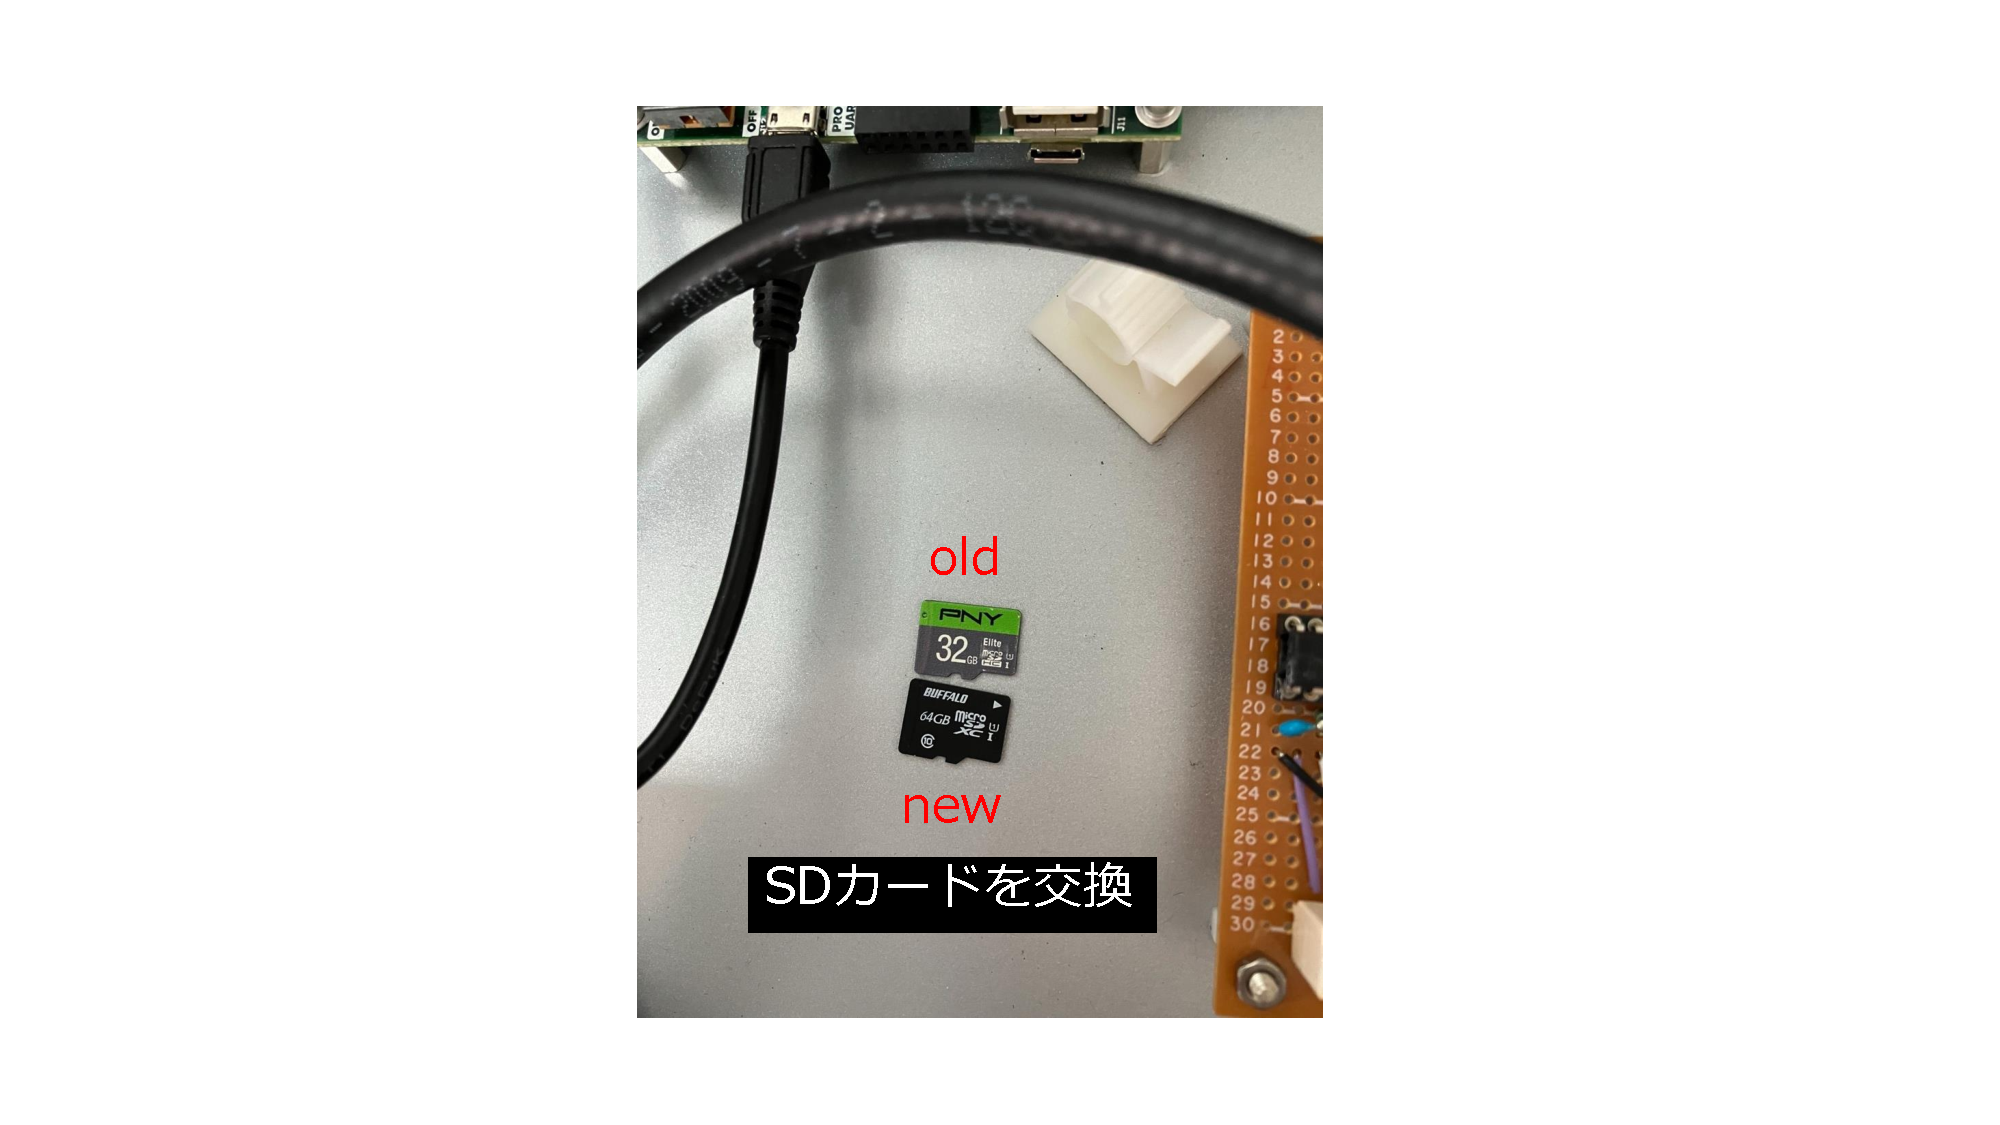
\includegraphics[keepaspectratio, scale=0.35]{4_elDAQ/figs/sd_exchange.pdf}
      \subcaption{SDカードの交換}
    \end{minipage}
    %---- 2番目の図 --------------------------
    \begin{minipage}[t]{0.45\hsize}
      \centering
      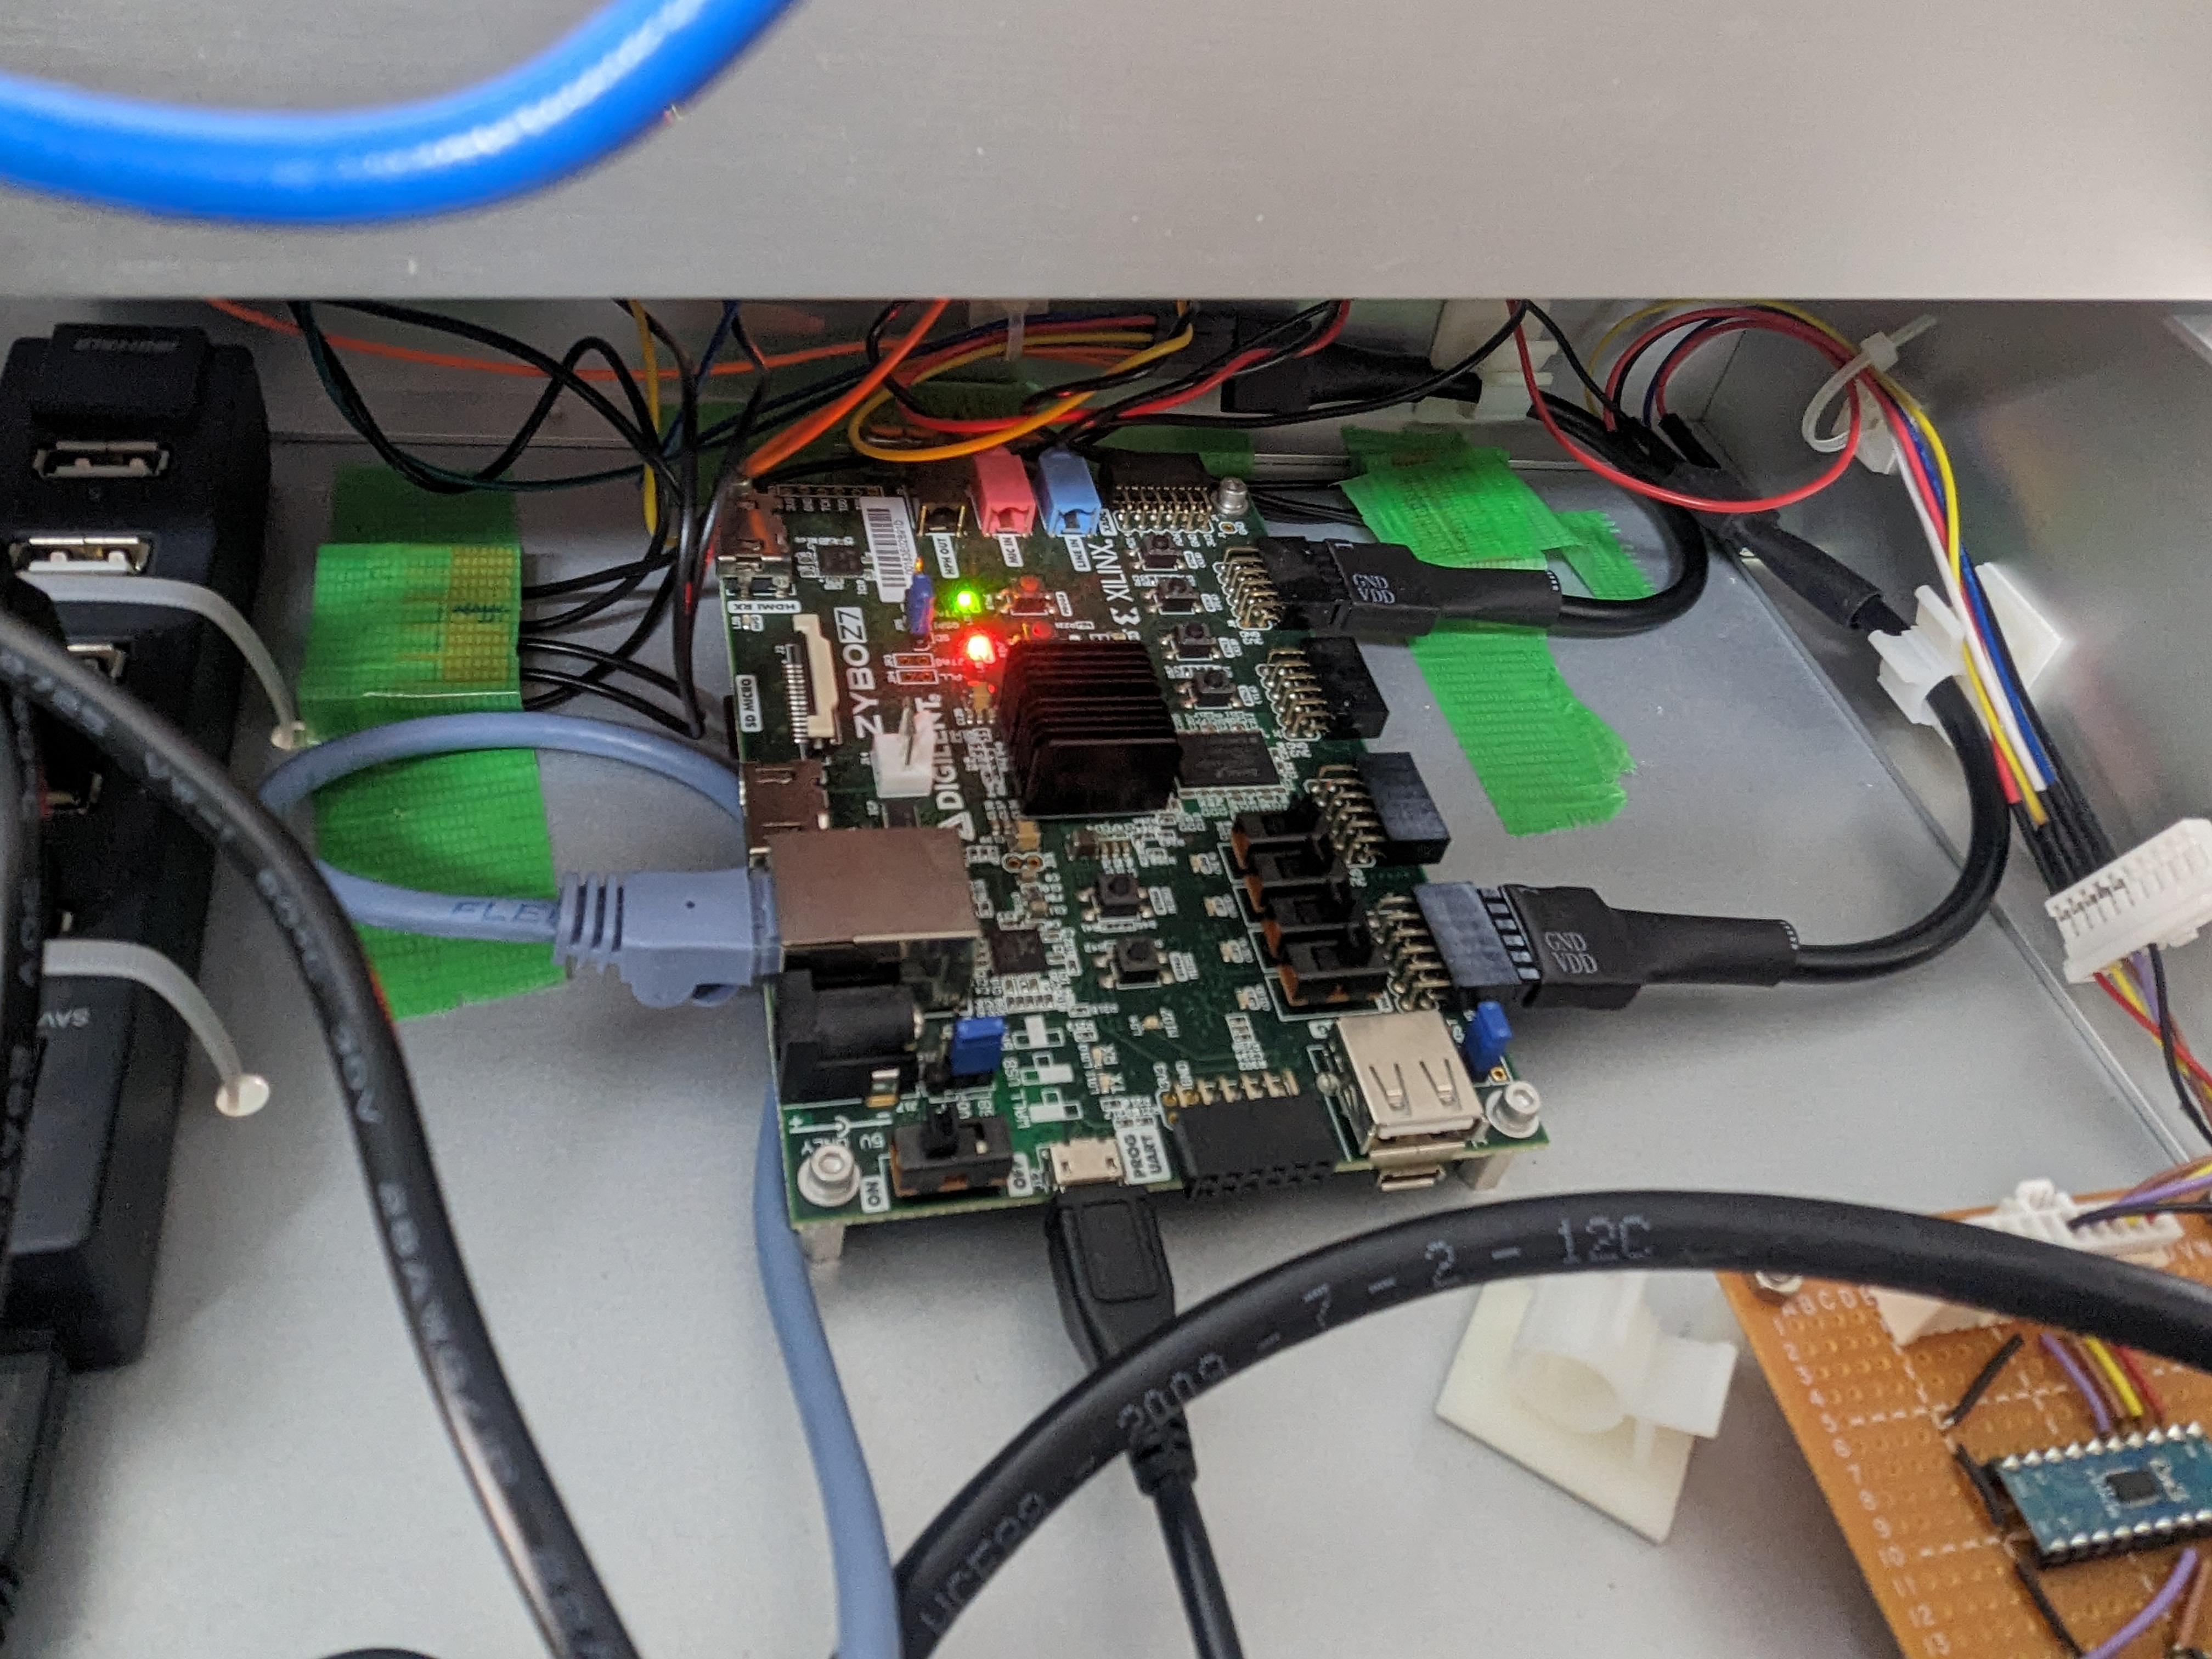
\includegraphics[keepaspectratio, scale=0.048]{4_elDAQ/figs/pynq_start.jpg}
      \subcaption{PYNQの起動}
    \end{minipage}
    %---- 図はここまで ----------------------
  \end{tabular}
  \vspace{5pt}
  \caption{新システムのインストール}
  \label{el_install}
\end{figure}

\subsection{同期信号取得の確認}
インストール後に実際の望遠鏡システムでデータを読み出せるかの動作確認を行なった。まず、方位角DAQからの同期信号を正しく取得して仰角データとして保存できているのかを確認した。結果を図\ref{sync_id}に示す。同期信号は1秒に1回出力されるので、仰角データでは同期信号の番号(図では``Sync\_id''と記す)が1秒で1ずつ増加する形で見えるはずであり、その結果を確認することができた。

\begin{figure}[htbp]
  \centering
  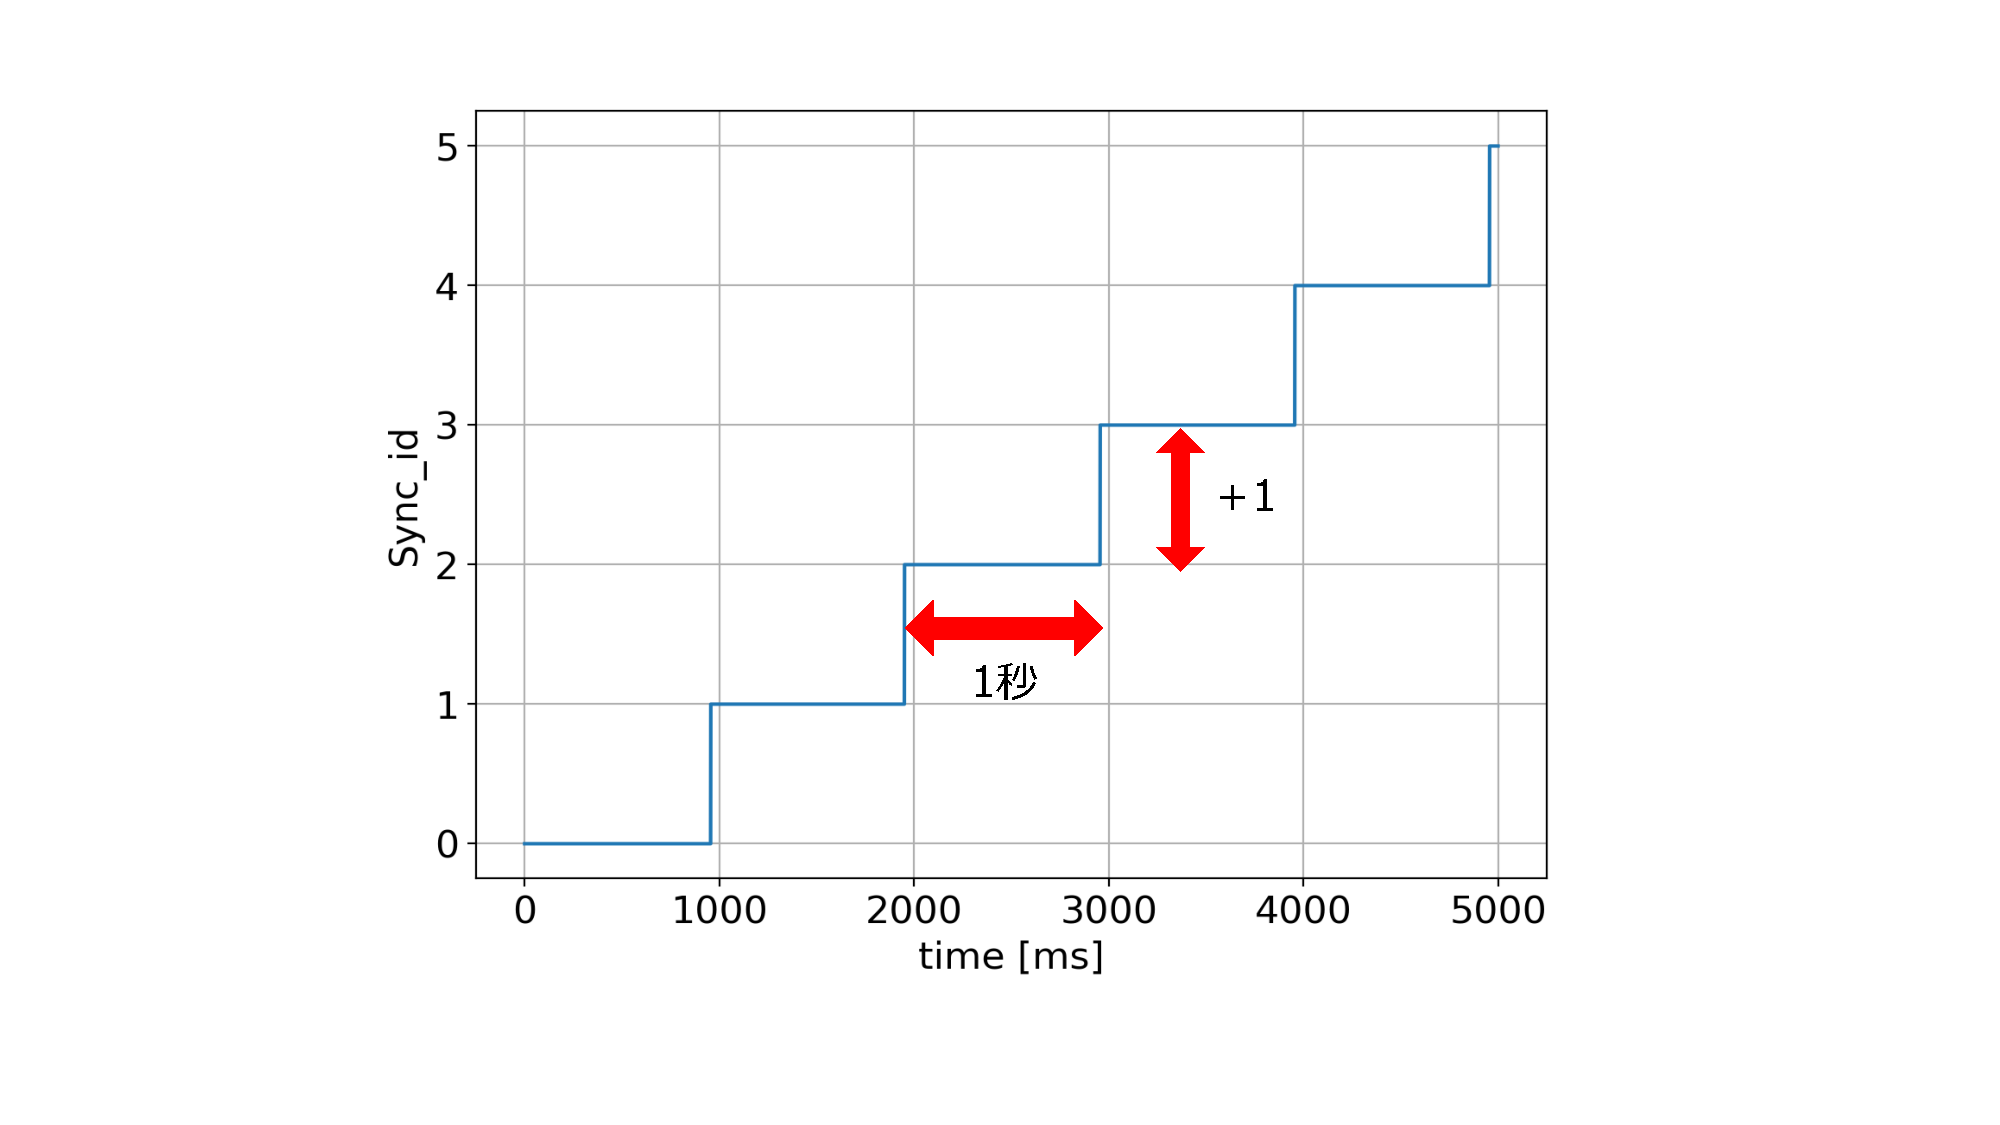
\includegraphics[width=0.8\columnwidth]{4_elDAQ/figs/sync_id.pdf}
  \caption{仰角データからみた同期信号。方位角DAQからの同期信号を取得するごとに``Sync\_id''が1ずつ加算される。}
  \label{sync_id}
\end{figure}

\subsection{同期信号の分配と仰角データ取得の確認}
次に、取得した同期信号をMKID DAQに分配できていることと仰角データを正しく読み出せているかを確認した。一度失ったエンコーダーの原点情報を再度取得するためにも、望遠鏡の仰角を$\SI{90}{^{\circ}}$と$\SI{70}{^{\circ}}$の間で何度か動かして、さらに並行してMKIDのデータも取得した。それらのデータを使って確認を行なった。確認の手順は以下である。
\begin{enumerate}
  \item テスト用として取ったMKIDデータを読み出す
  \item 正しく動作していればMKIDデータに同期した時間情報と仰角データを取得できる
  \item その仰角データが正しい値を読み出せているかを確認
\end{enumerate}

結果を図\ref{elevation_data}に示す。MKIDデータから同期情報を取得でき、読み出した仰角データが$\SI{90}{^{\circ}}$と$\SI{70}{^{\circ}}$の間で正しく動いていることも確認した。

\begin{figure}[htbp]
  \centering
  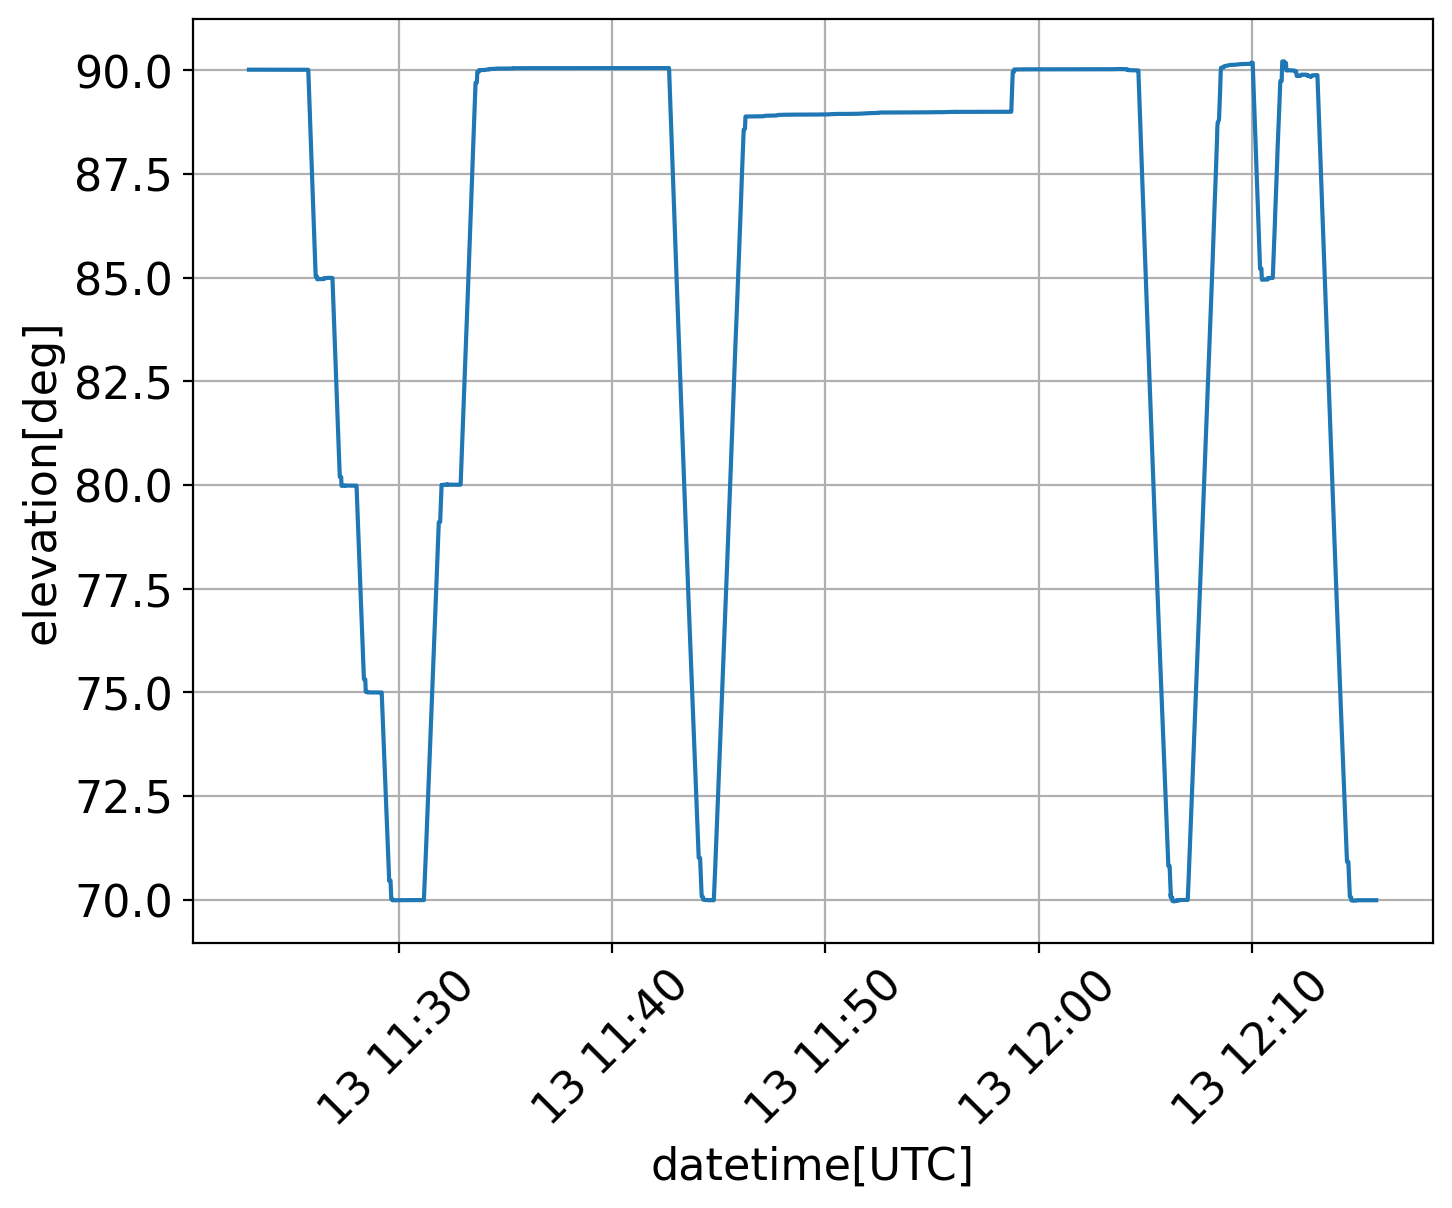
\includegraphics[width=0.8\columnwidth]{4_elDAQ/figs/elevation_data.png}
  \caption{読み出した仰角データ。横軸(2024/3/13のUTC時間)の時間情報が実際の作業時間とリンクしており、MKIDデータで同期信号が正しく取得できていることを反映している。}
  \label{elevation_data}
\end{figure}

以上から新システムが実際の望遠鏡で問題なく動作することを確認した。その後、動作が安定して長期間行われるかをチェックした。

\section{メンテナンスと安定運用}

\subsection{動作の不安定性}
インストール後、動作の安定性に問題があり、データ取得が途切れることが何度か発生した。途切れる原因はZyboの電源が一時的(データ取得開始後数時間)に落ちることによるものであった。インストール時の動作確認で問題がなかったことから、Zynq内でのデータ処理と通信自体に問題がある可能性はないと考えた。他に原因となりうるものは
\begin{itemize}
  \item OSが搭載されたことでZyboの消費電力が上がり、一時的に電源供給量が足りなくなる
  \item Zynqでの消費電力も上がり、Zynqの温度が許容値よりも高くなってしまう
  \item そもそもZyboのボード自体がどこかで劣化している
\end{itemize}
が挙げられる。3つ目に関しては、経年劣化や落雷による停電時にダメージを受けたことなどが考えられるが、リモートからボード自体の性能を評価することが難しいため、まずは1つ目と2つ目の要因について調査した。結果として、1つ目の電源供給が原因である可能性が高いことが分かった。

\subsection{電源供給方法の見直し}
\label{power_sup}
Zyboへの電源供給は図\ref{el_install}の右図にあるように、Micro-USB端子から行なっていた。Zyboへの電源供給方法は他にバレルジャックから(図\ref{power_supply})がある。

\begin{figure}[htbp]
  \centering
  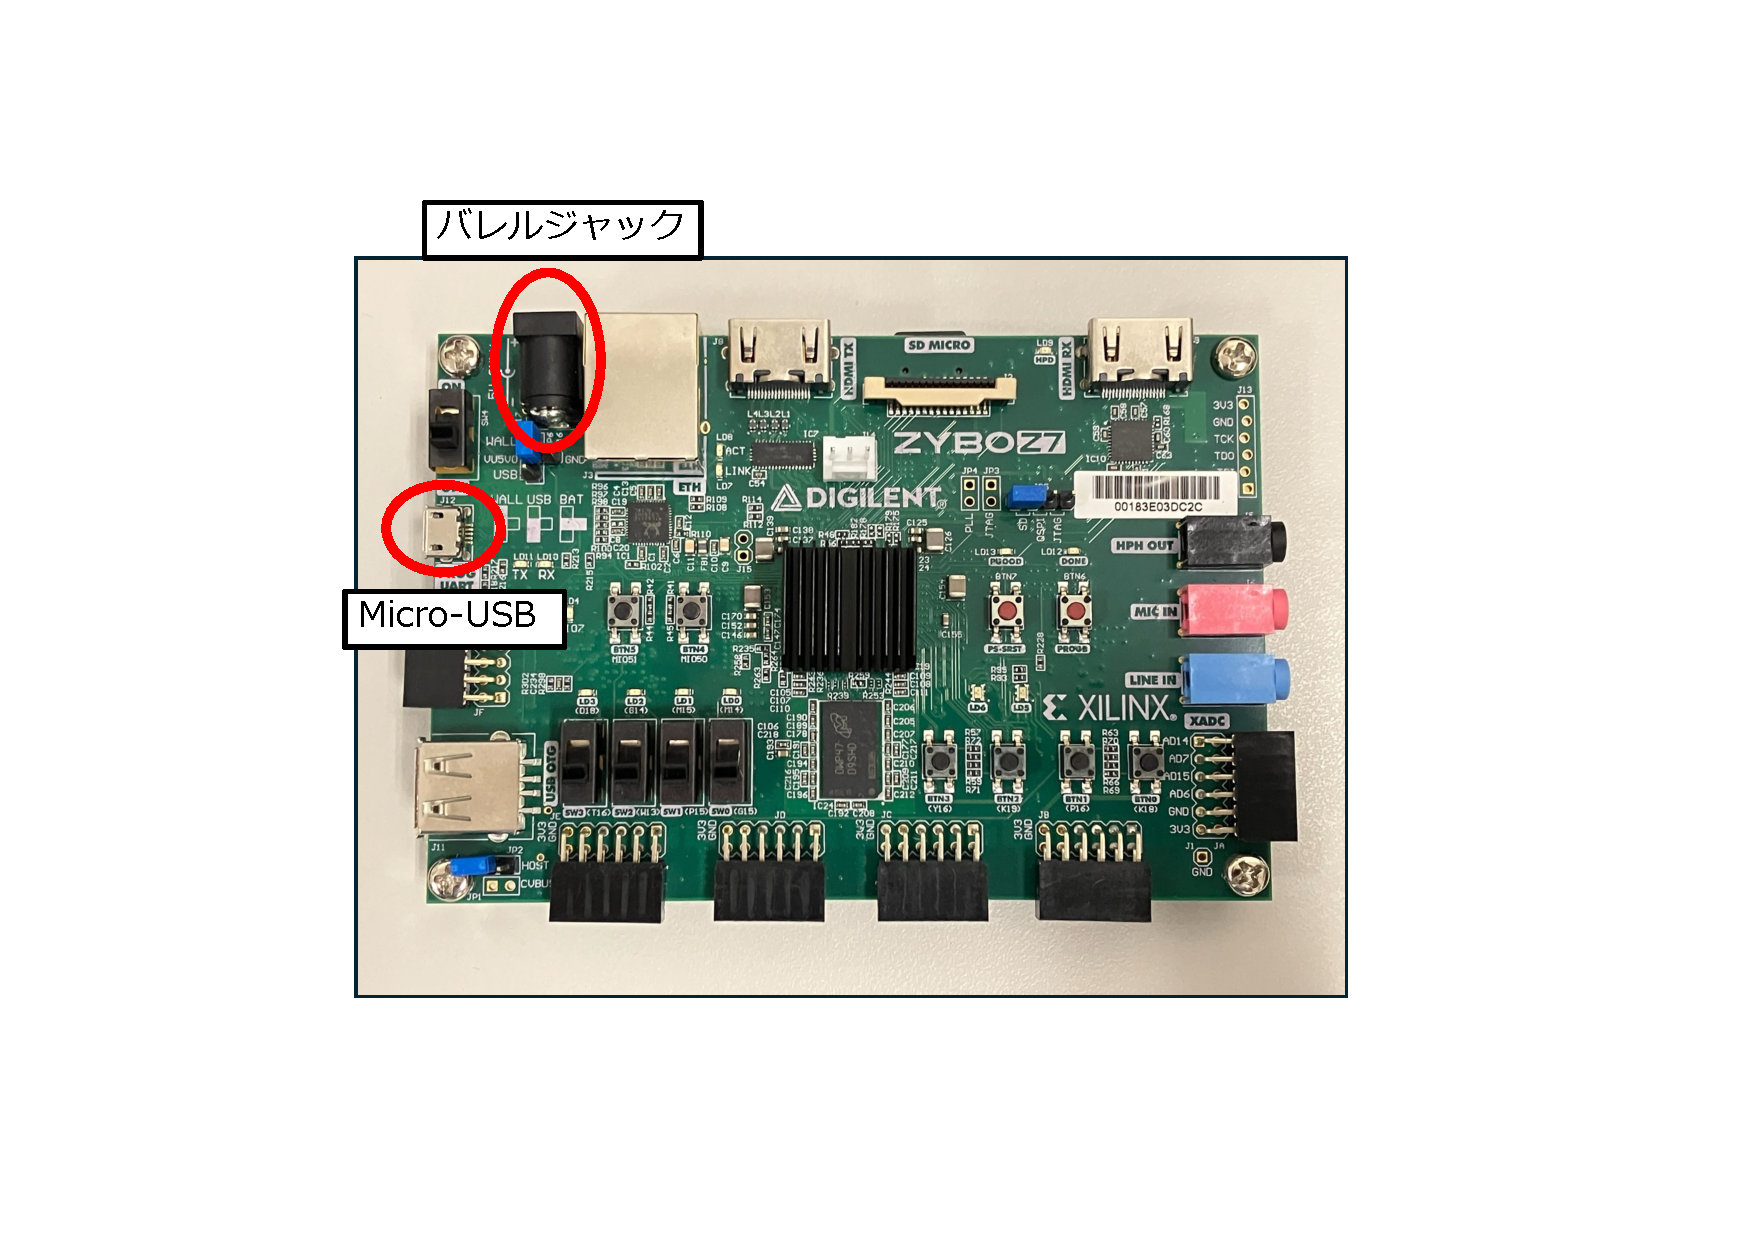
\includegraphics[width=0.5\columnwidth]{4_elDAQ/figs/connector_barrel.pdf}
  \caption{Zyboへの電源供給方法。Micro-USBからとバレルジャックからの2通りがある。}
  \label{power_supply}
\end{figure}

この2種類の供給方法について比較すると表\ref{power_spec}のようになる。バレルジャックについては標準的なACアダプタの規格を参照する。

\begin{table}[htbp]
  \centering
  \caption{各電源供給方法での定格値}
  \vspace{3mm}
  \begin{tabular}{cccc} \hline\hline
    供給方法 & 定格電圧 & 定格電流 & 接続の安定性  \\ \hline
    Micro-USB & \SI{5}{V} & 最大\SI{0.5}{A} & やや不安定\\
    バレルジャック & \SI{5}{V} & 最大\SI{4}{A} &  安定\\ \hline\hline
  \end{tabular}
  \label{power_spec}
\end{table}

これより、供給できる電力量や接続の安定性に関してバレルジャックの方が優れていることが分かる。特に定格電流の値が大きく異なっており、従来のシステムではMicro-USBからの給電で間に合っていたが、OSが搭載されたことで給電が足りなくなった可能性が考えられる。スペックシート\cite{power_ref}でもバレルジャックによる電源供給が推奨されている(参考として、電力を大量に消費する処理をZynqに搭載した場合は\SI{12.5}{W}以上の出力が必要)。そのため、Zyboへの電源供給方法をバレルジャックに変更して十分な電力を供給することで動作の安定性を図るのが良いと考えた。変更するにあたって新システムを稼働した際のZyboの動作安定性を給電条件を変えてテストした。行なったテストの様子を図\ref{power_test}に、給電条件と結果を表\ref{power_result}に示す。

\begin{figure}[htbp]
  \begin{tabular}{cc}
    \begin{minipage}[t]{0.45\hsize}
      \centering
      \includegraphics[width=0.8\columnwidth]{4_elDAQ/figs/test_usb.jpg}
      \subcaption{テスト1}
    \end{minipage} &
    \begin{minipage}[t]{0.45\hsize}
      \centering
      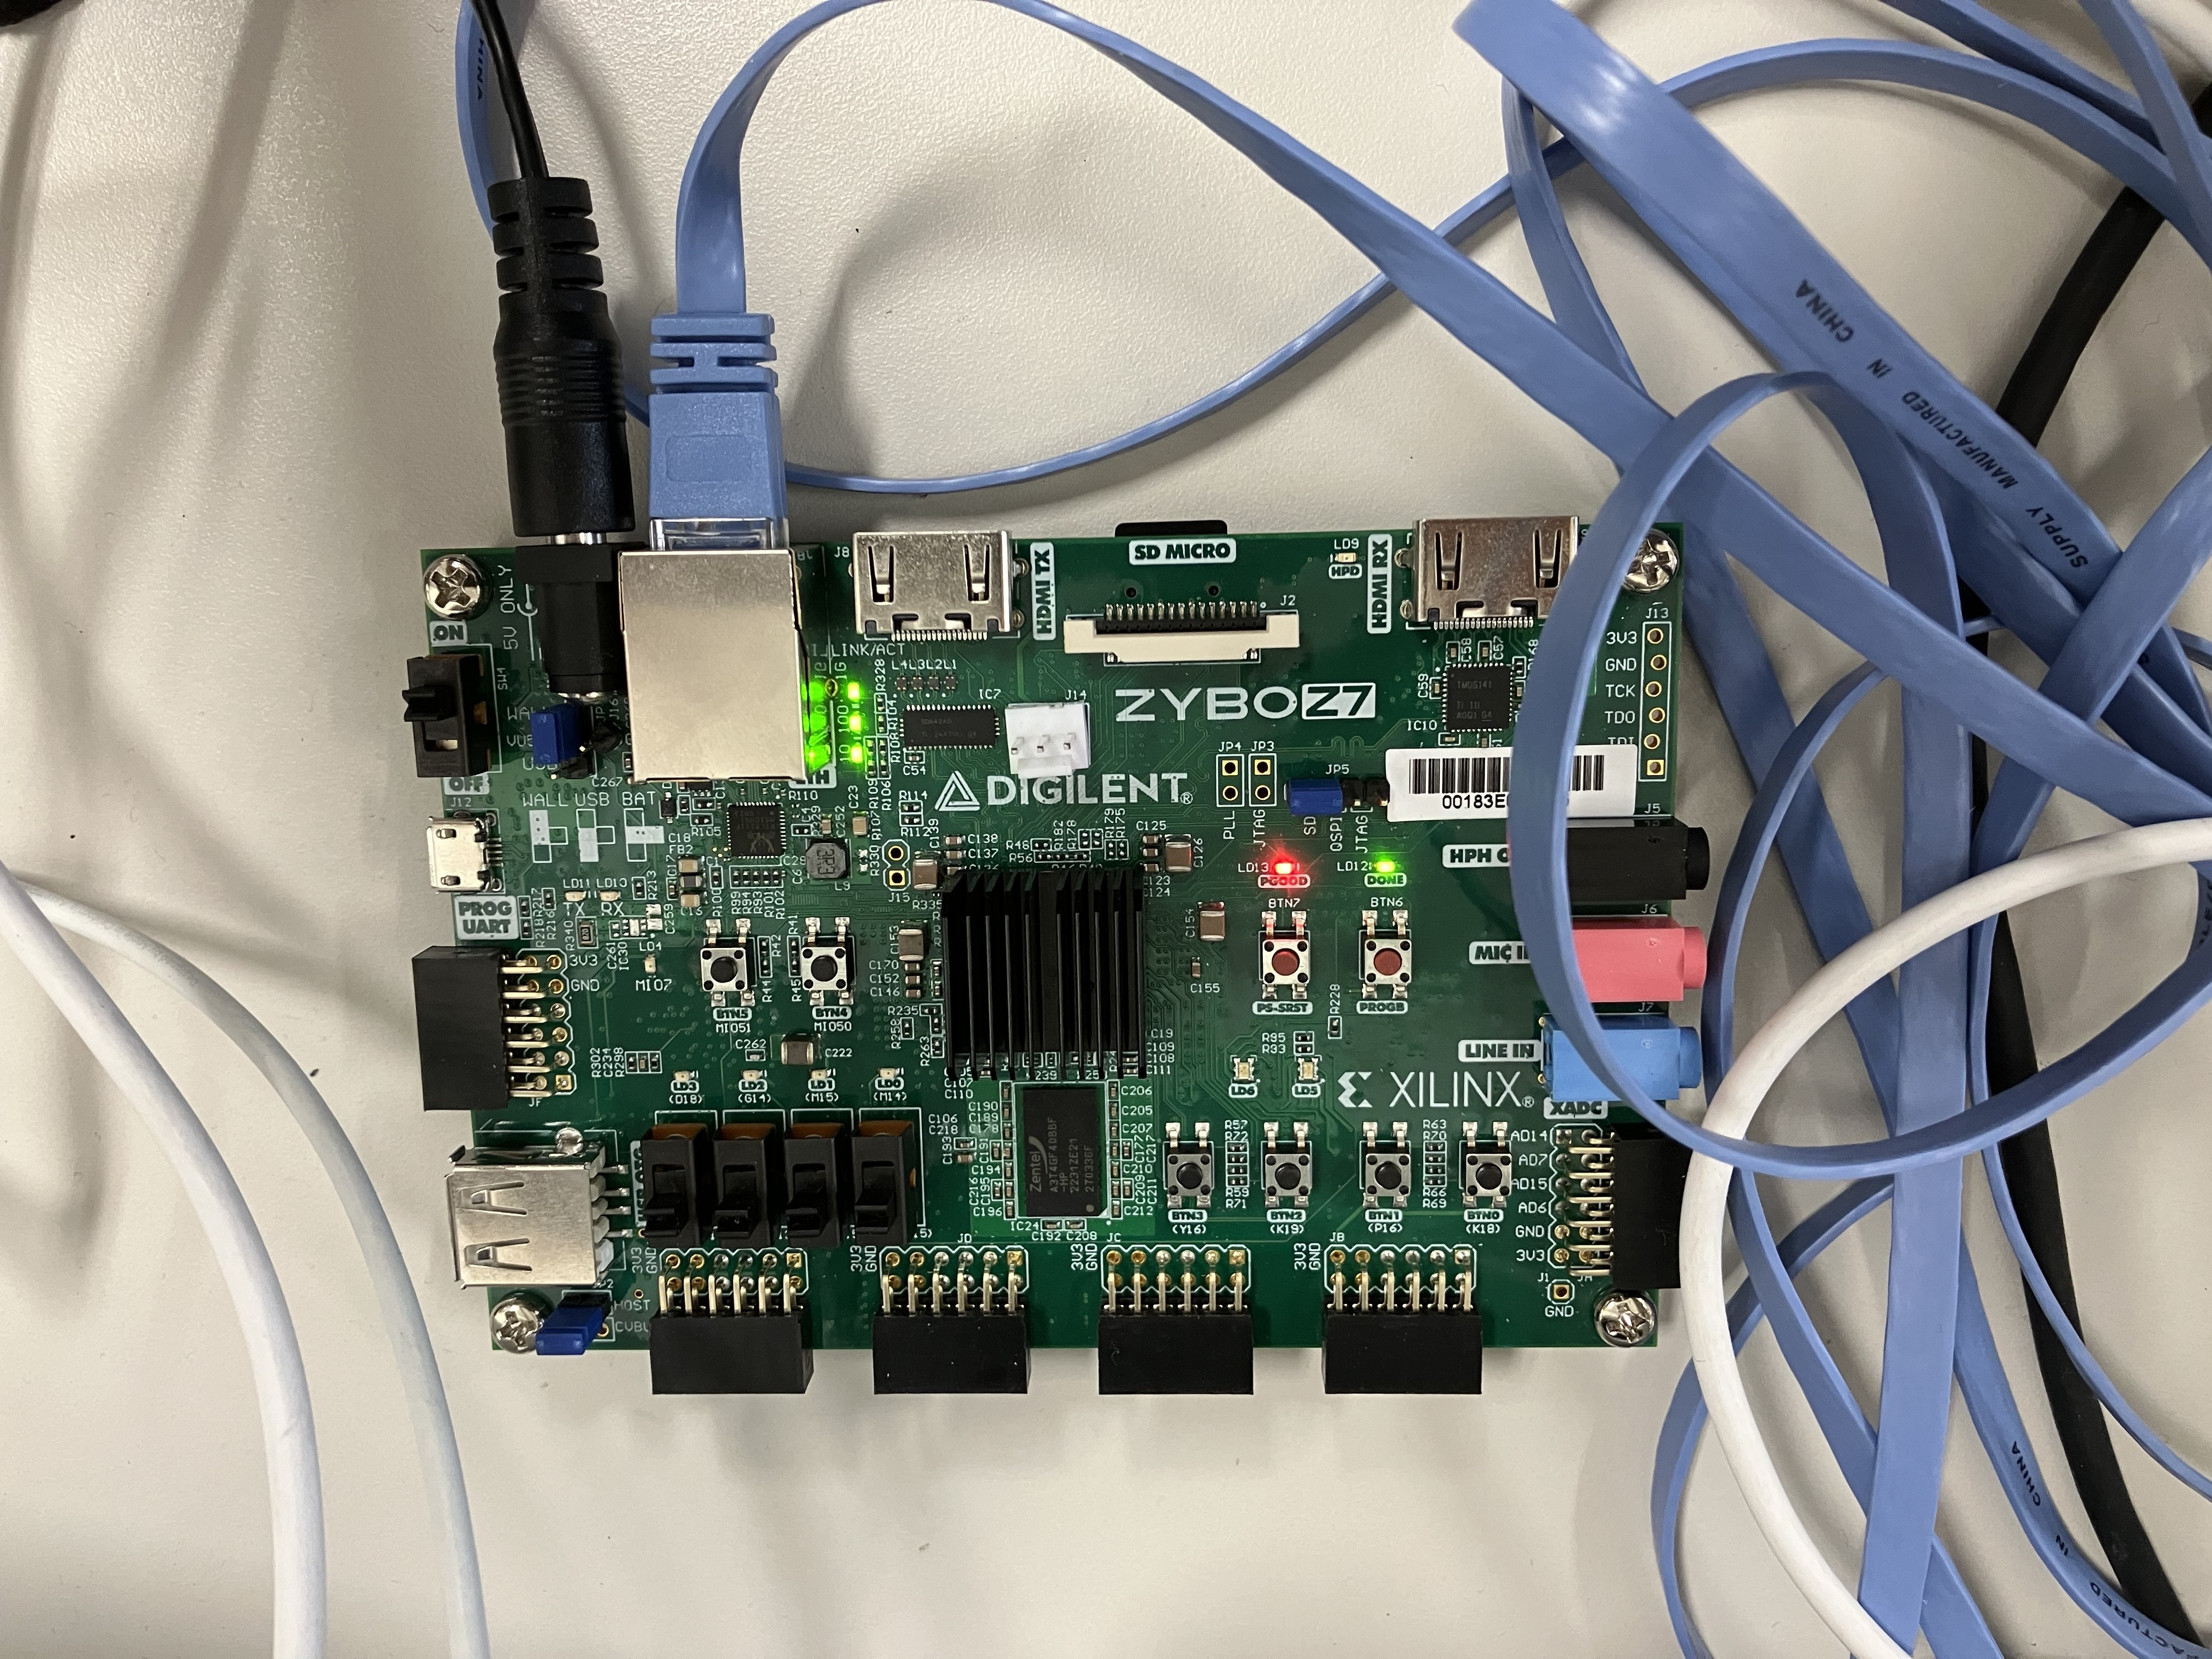
\includegraphics[width=0.8\columnwidth]{4_elDAQ/figs/test_jack.jpg}
      \subcaption{テスト2}
    \end{minipage} \\

    \begin{minipage}[t]{0.45\hsize}
      \centering
      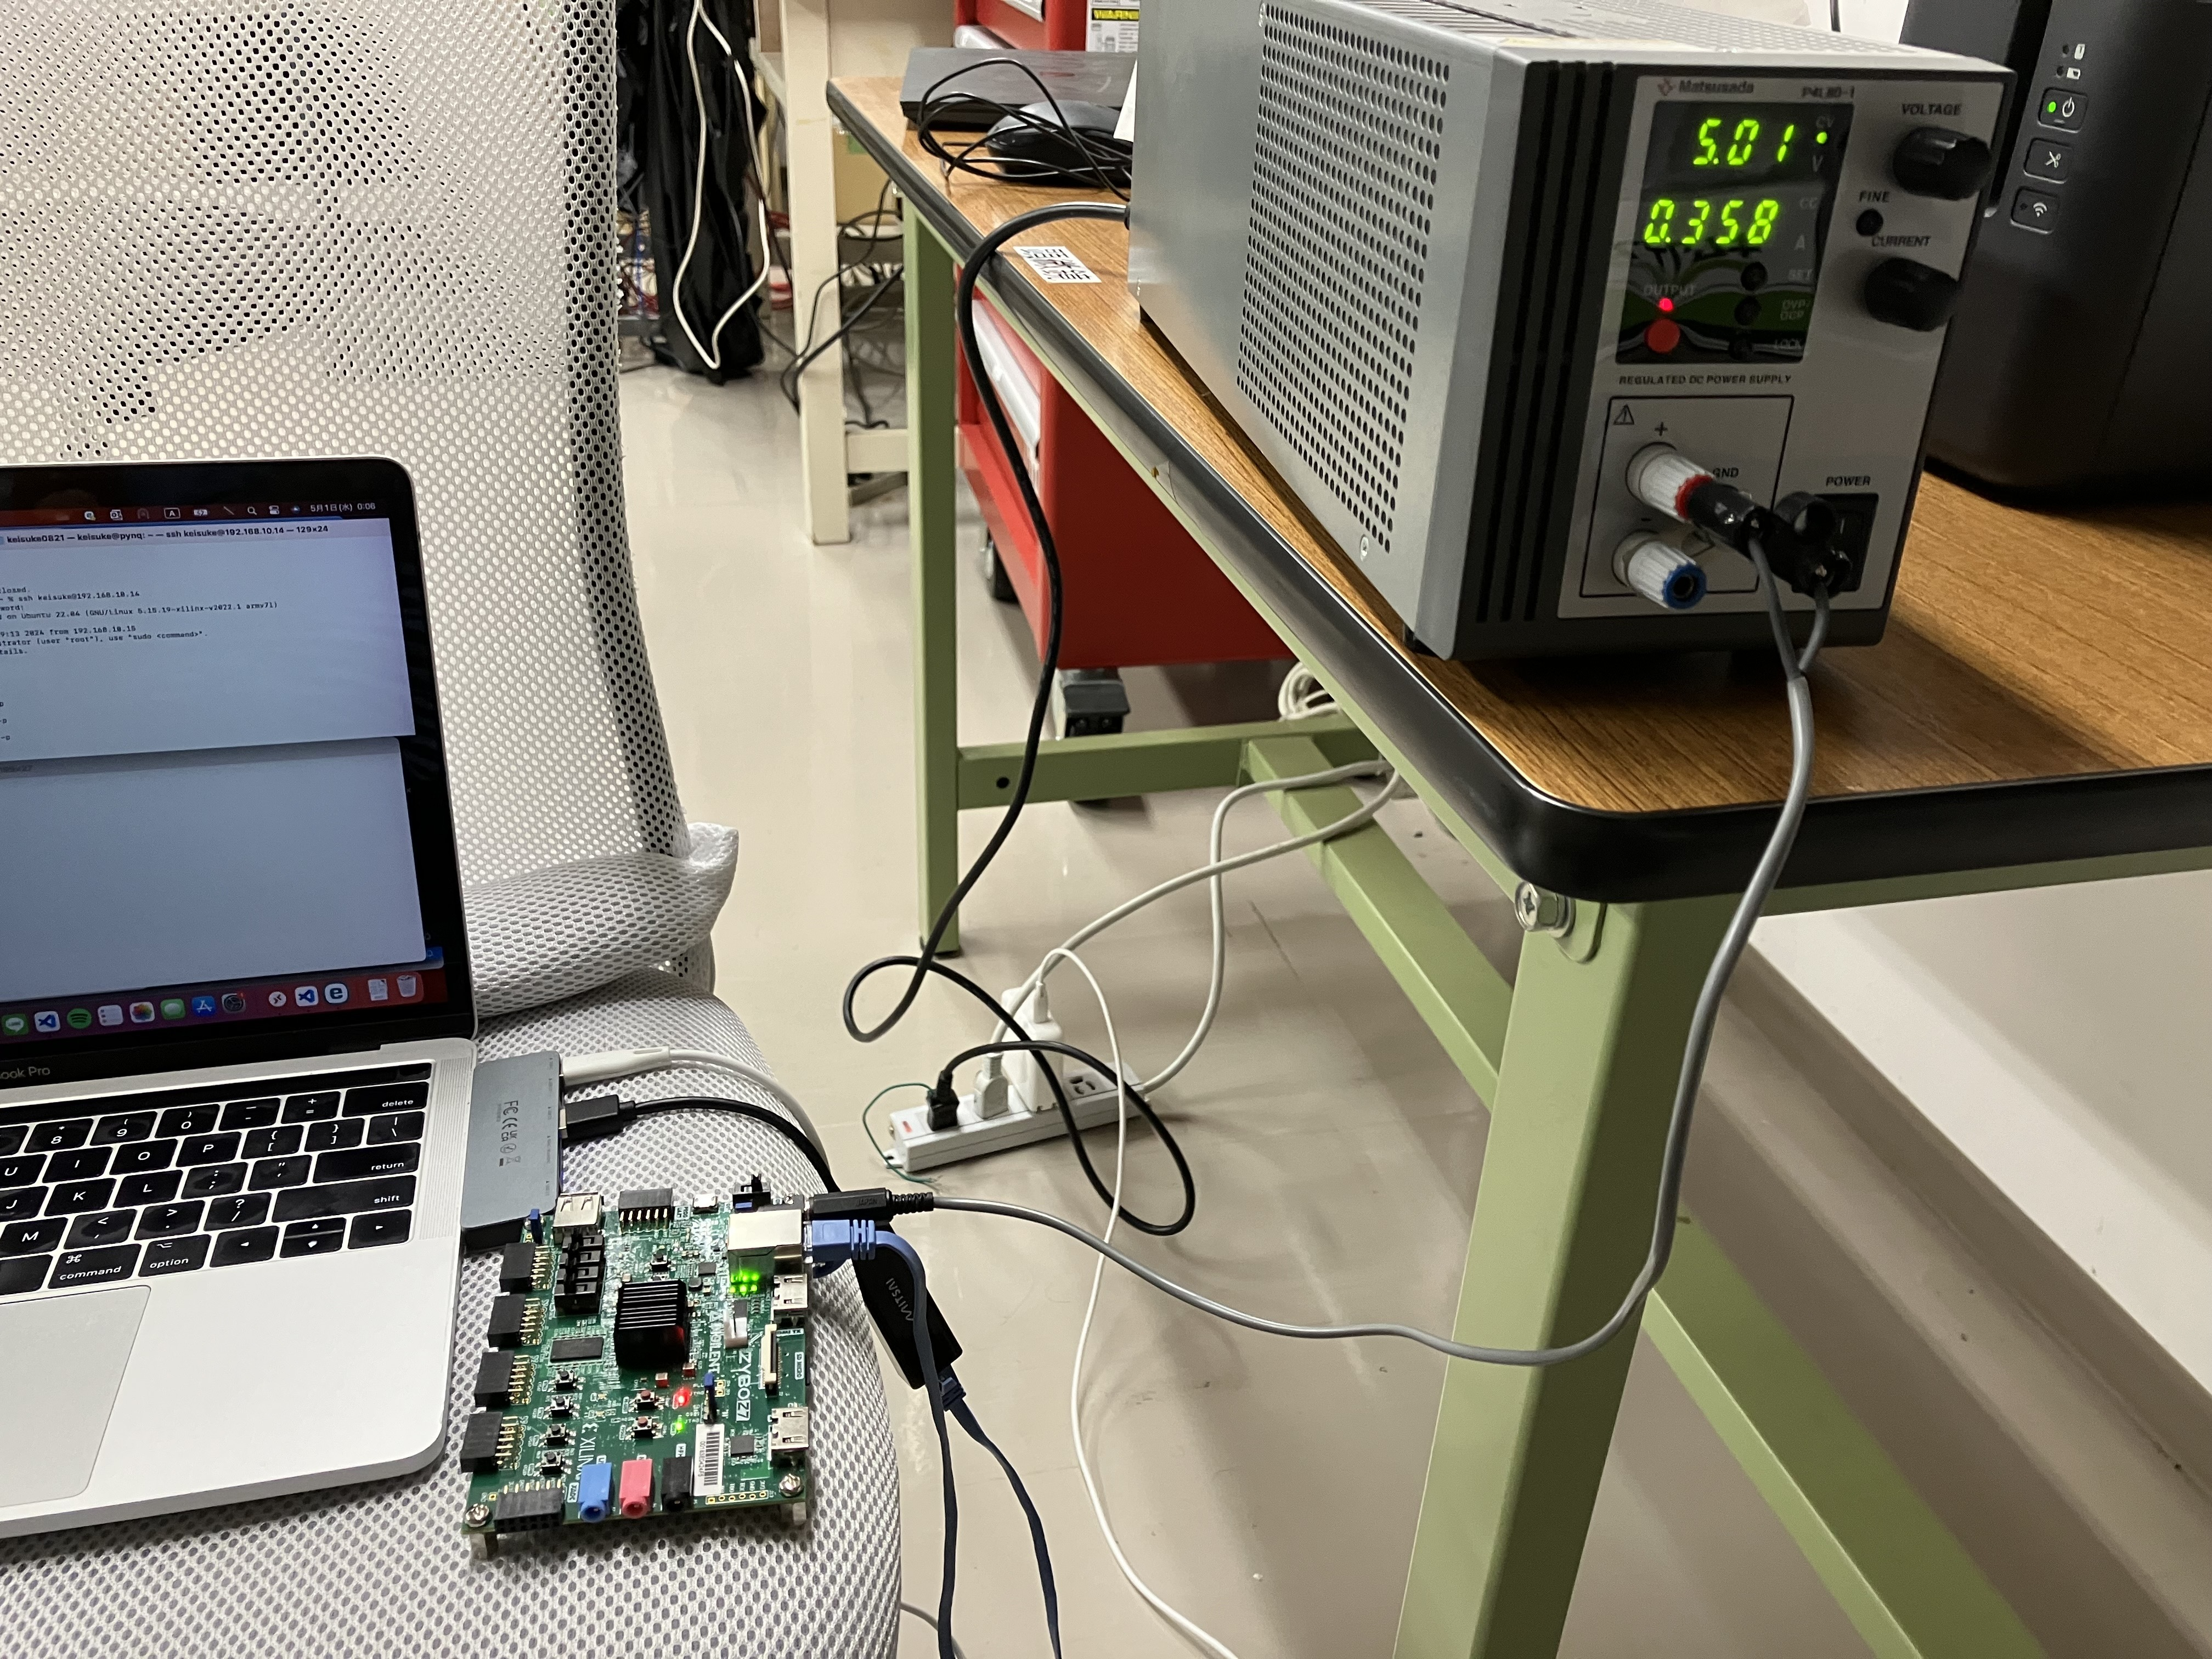
\includegraphics[width=0.8\columnwidth]{4_elDAQ/figs/test_50.jpg}
      \subcaption{テスト3}
    \end{minipage} &
    \begin{minipage}[t]{0.45\hsize}
      \centering
      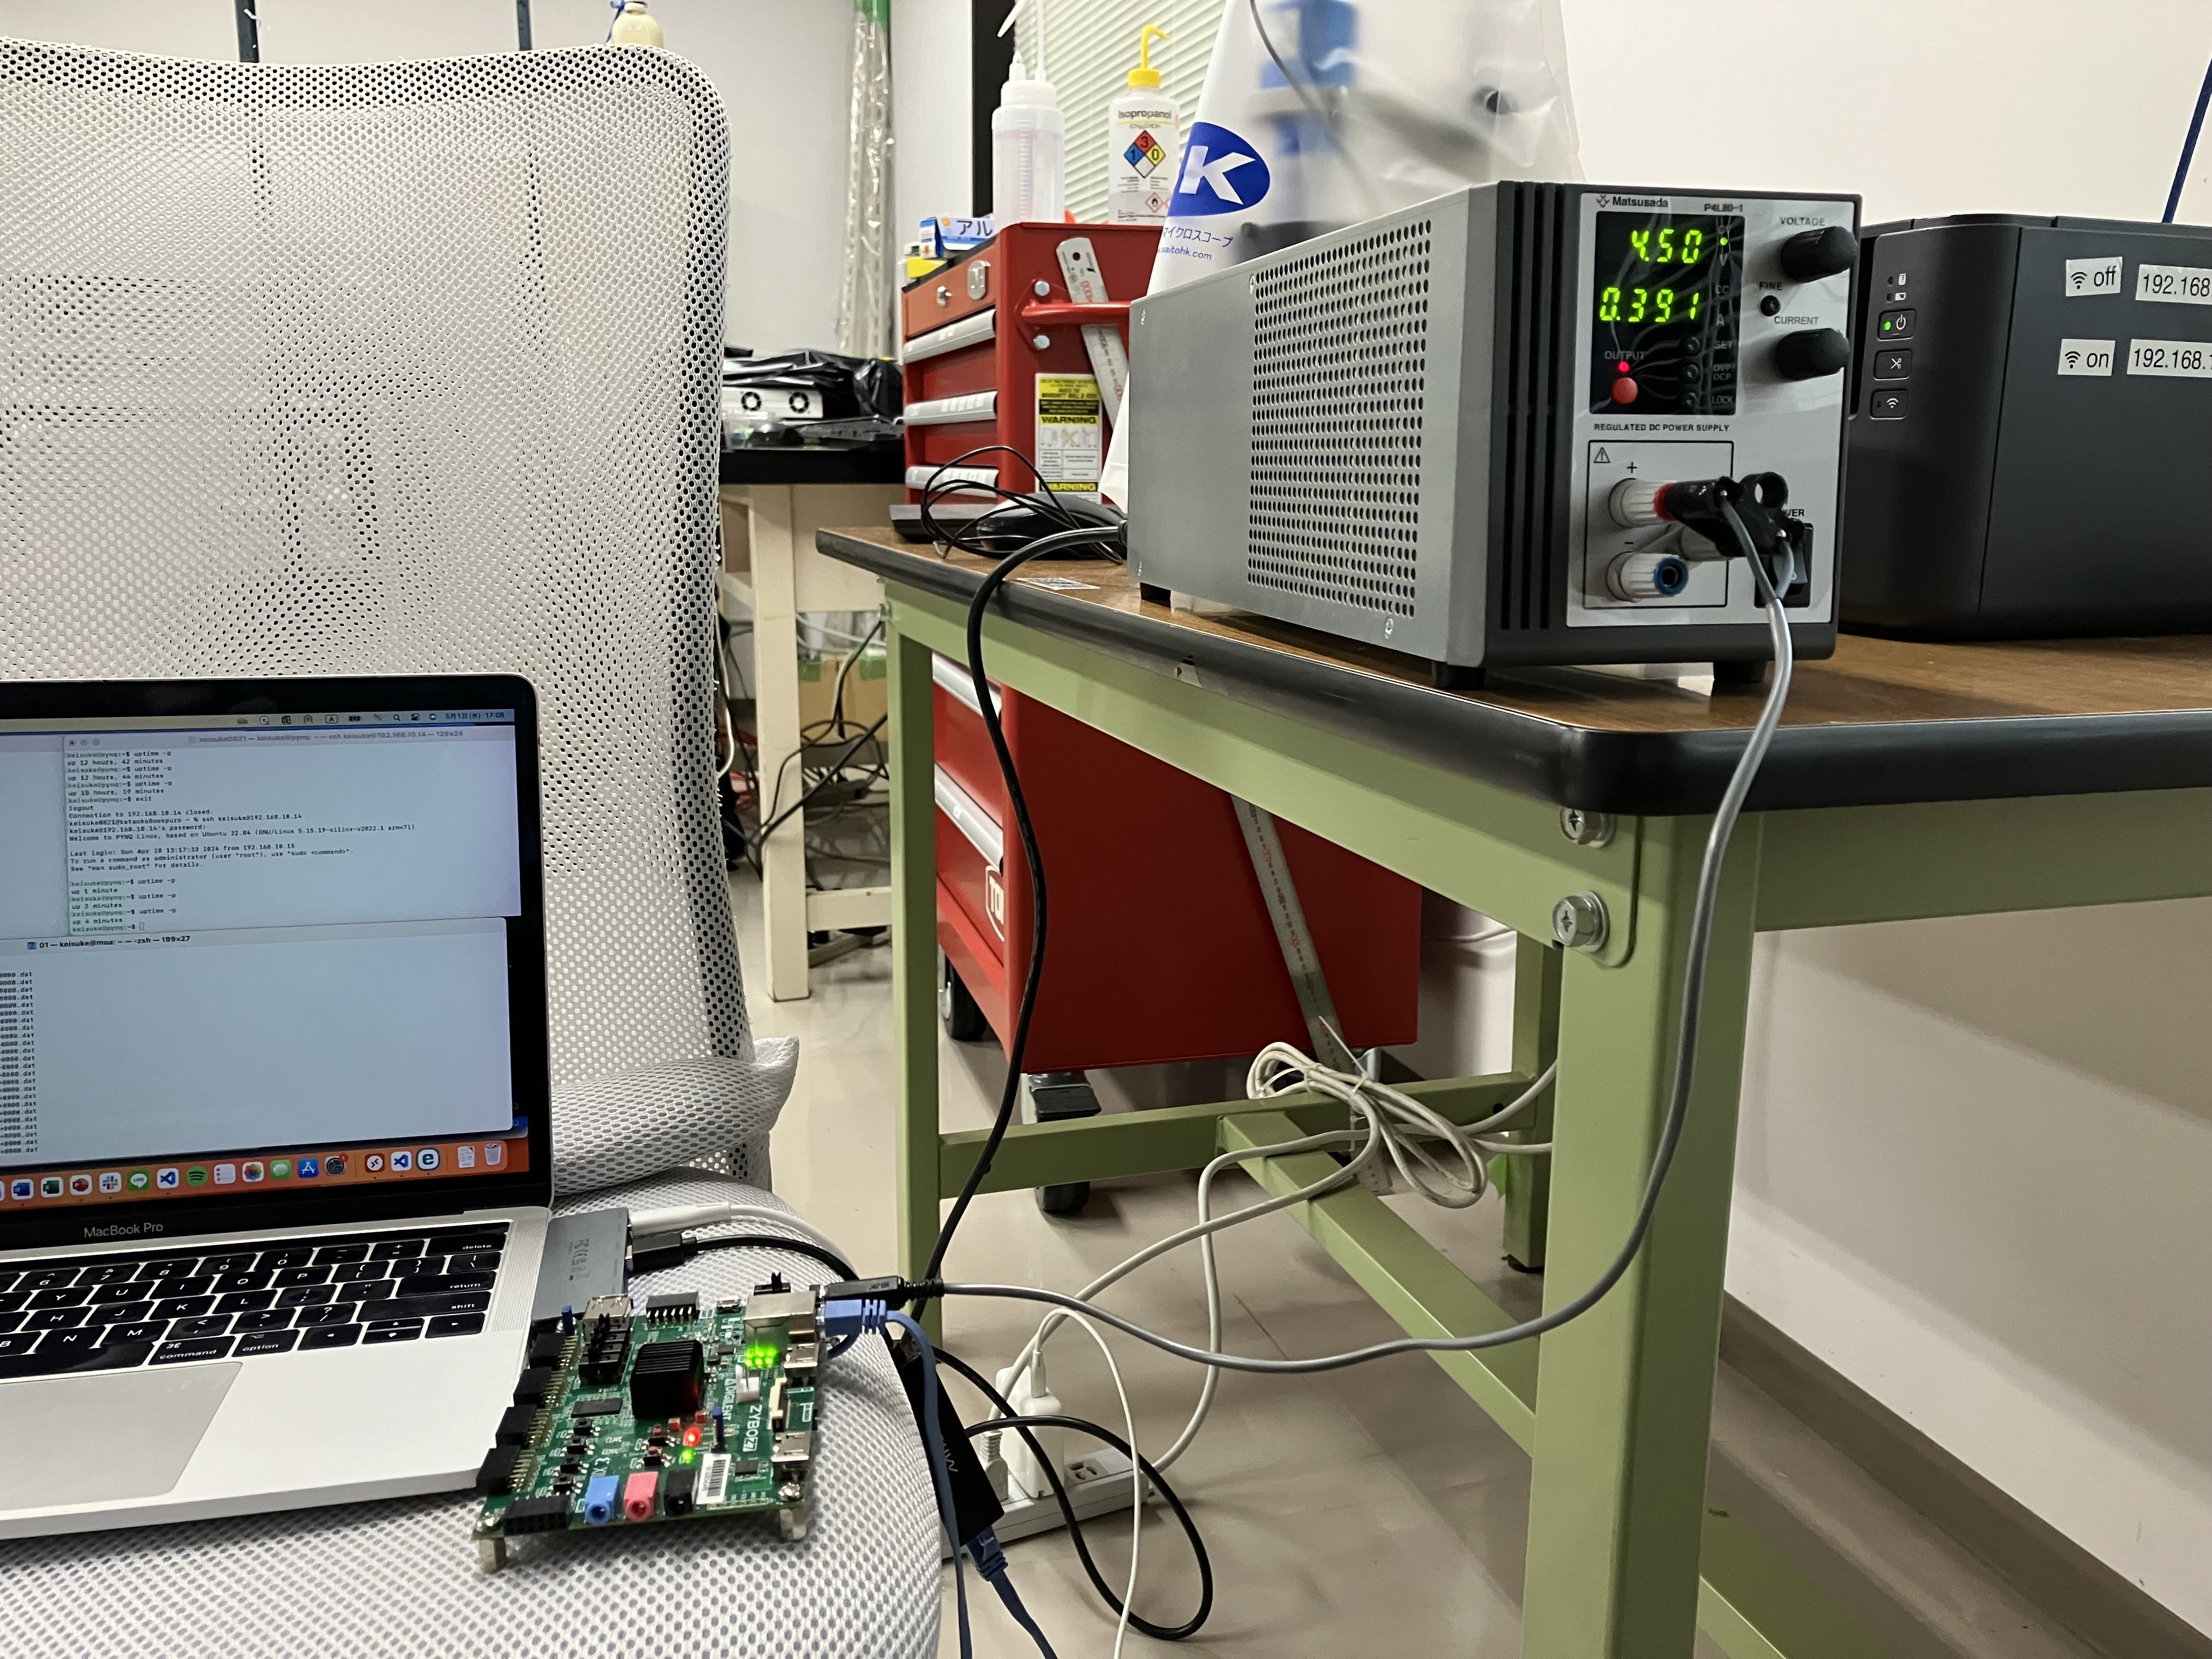
\includegraphics[width=0.8\columnwidth]{4_elDAQ/figs/test_45.jpg}
      \subcaption{テスト4}
    \end{minipage}
  \end{tabular}
  \vspace{5pt}
   \caption{Zyboの安定稼働テスト}
   \label{power_test}
\end{figure}

\begin{table}[htbp]
  \centering
  \caption{安定稼働テストの給電条件と結果}
  \vspace{3mm}
  \begin{tabular}{ccc} \hline
     & 給電条件 & 動作の結果  \\ \hline
    テスト1 & 従来と同じUSB & 安定 \\
    テスト2 & バレルジャック(\SI{5}{V}、\SI{4}{A}のACアダプタ) & 安定 \\ \hline
    テスト3 & 直流電源(定電圧モード \SI{5.0}{V}) & 安定 \\
    テスト4 & 直流電源(定電圧モード \SI{4.5}{V}) & 不安定(数時間でZyboの電源が落ちる) \\ \hline
  \end{tabular}
  \label{power_result}
\end{table}

基本的なセットアップは図\ref{el_test}と同じで給電の条件のみが異なっている。テスト1では従来と同じでMicro-USBからの給電でデータ取得を動かし、数日にわたって動作の安定性を確認し、少なくとも3日以上はZyboの電源が落ちることなく稼働する結果を得た。これは現地で起きている問題と矛盾する結果となった。テスト2ではバレルジャックから給電し、こちらも安定した稼働をすることを確認した。稼働が不安定である原因が特定できなかったため、条件を変え、さらに検証を行なった。

テスト3と4では直流電源(松定プレシジョン製)を使用し、与える電圧値を変えて稼働の安定性を確認した。USBの定格電圧が\SI{5}{V}であることと、Zyboで推奨されている供給電圧が\SI{4.5}{V}$\sim$ \SI{5.5}{V}であることから\SI{5.0}{V}と\SI{4.5}{V}を設定した。電源を定電圧モードにすることで電流値はZyboでデータ取得システムを動かすために必要な電流量になる。テスト3では\SI{5.0}{V}で行い、安定した稼働結果と電流値$\sim$ \SI{0.36}{A}を得た。テスト4では\SI{4.5}{V}で行い、データ取得開始後数時間でZyboの電源が落ちる事象が複数回起き、現地での問題と同様の挙動を確認した。また、稼働中の電流値は$\sim$ \SI{0.39}{A}であった。これより、データ取得システムの稼働に必要な電力量は比較的少ないことが分かるが、実際はエンコーダーデータと同期信号を取得し処理しているため、消費電力がこれよりも少なからず増えると考えれば、システムの稼働にはMicro-USBの定格電流値の\SI{0.5}{A}に近い電流量が必要になる。

テストの結果を踏まえると、Zyboへの供給電圧が定格通り\SI{5.0}{V}であればシステム稼働に必要な電流量がUSBの定格電流値を下回り十分な電力を供給できるが、電圧値のふらつきで\SI{5.0}{V}より小さくなると、稼働に必要な電力量を保持するために電流量が増加し、定格電流値に近づくためにUSBでの給電が一時的に不足してZyboの電源が落ちる可能性があると言える\footnote{Zynq内蔵の``XADC''でZynqへの供給電圧をモニターできるが、Zybo全体への供給電圧をモニターできるわけではないため、実際のデータ取得システムに供給される電圧、電流値を正確に知る手法は確立できなかった。}。そのため、性能面に加えて、実際の問題への対処という意味でもバレルジャックに変更することの妥当性を検証することができた。

Zyboへの電源供給をMicro-USBからバレルジャックに変更し(図\ref{new_connector})、システムを再起動させた。その後、動作が安定することを確認した。再起動して以降、半年以上の安定動作を続けている。

\begin{figure}[h]
  \begin{tabular}{cc}
    %---- 最初の図 ---------------------------
    \begin{minipage}[t]{0.45\hsize}
      \centering
      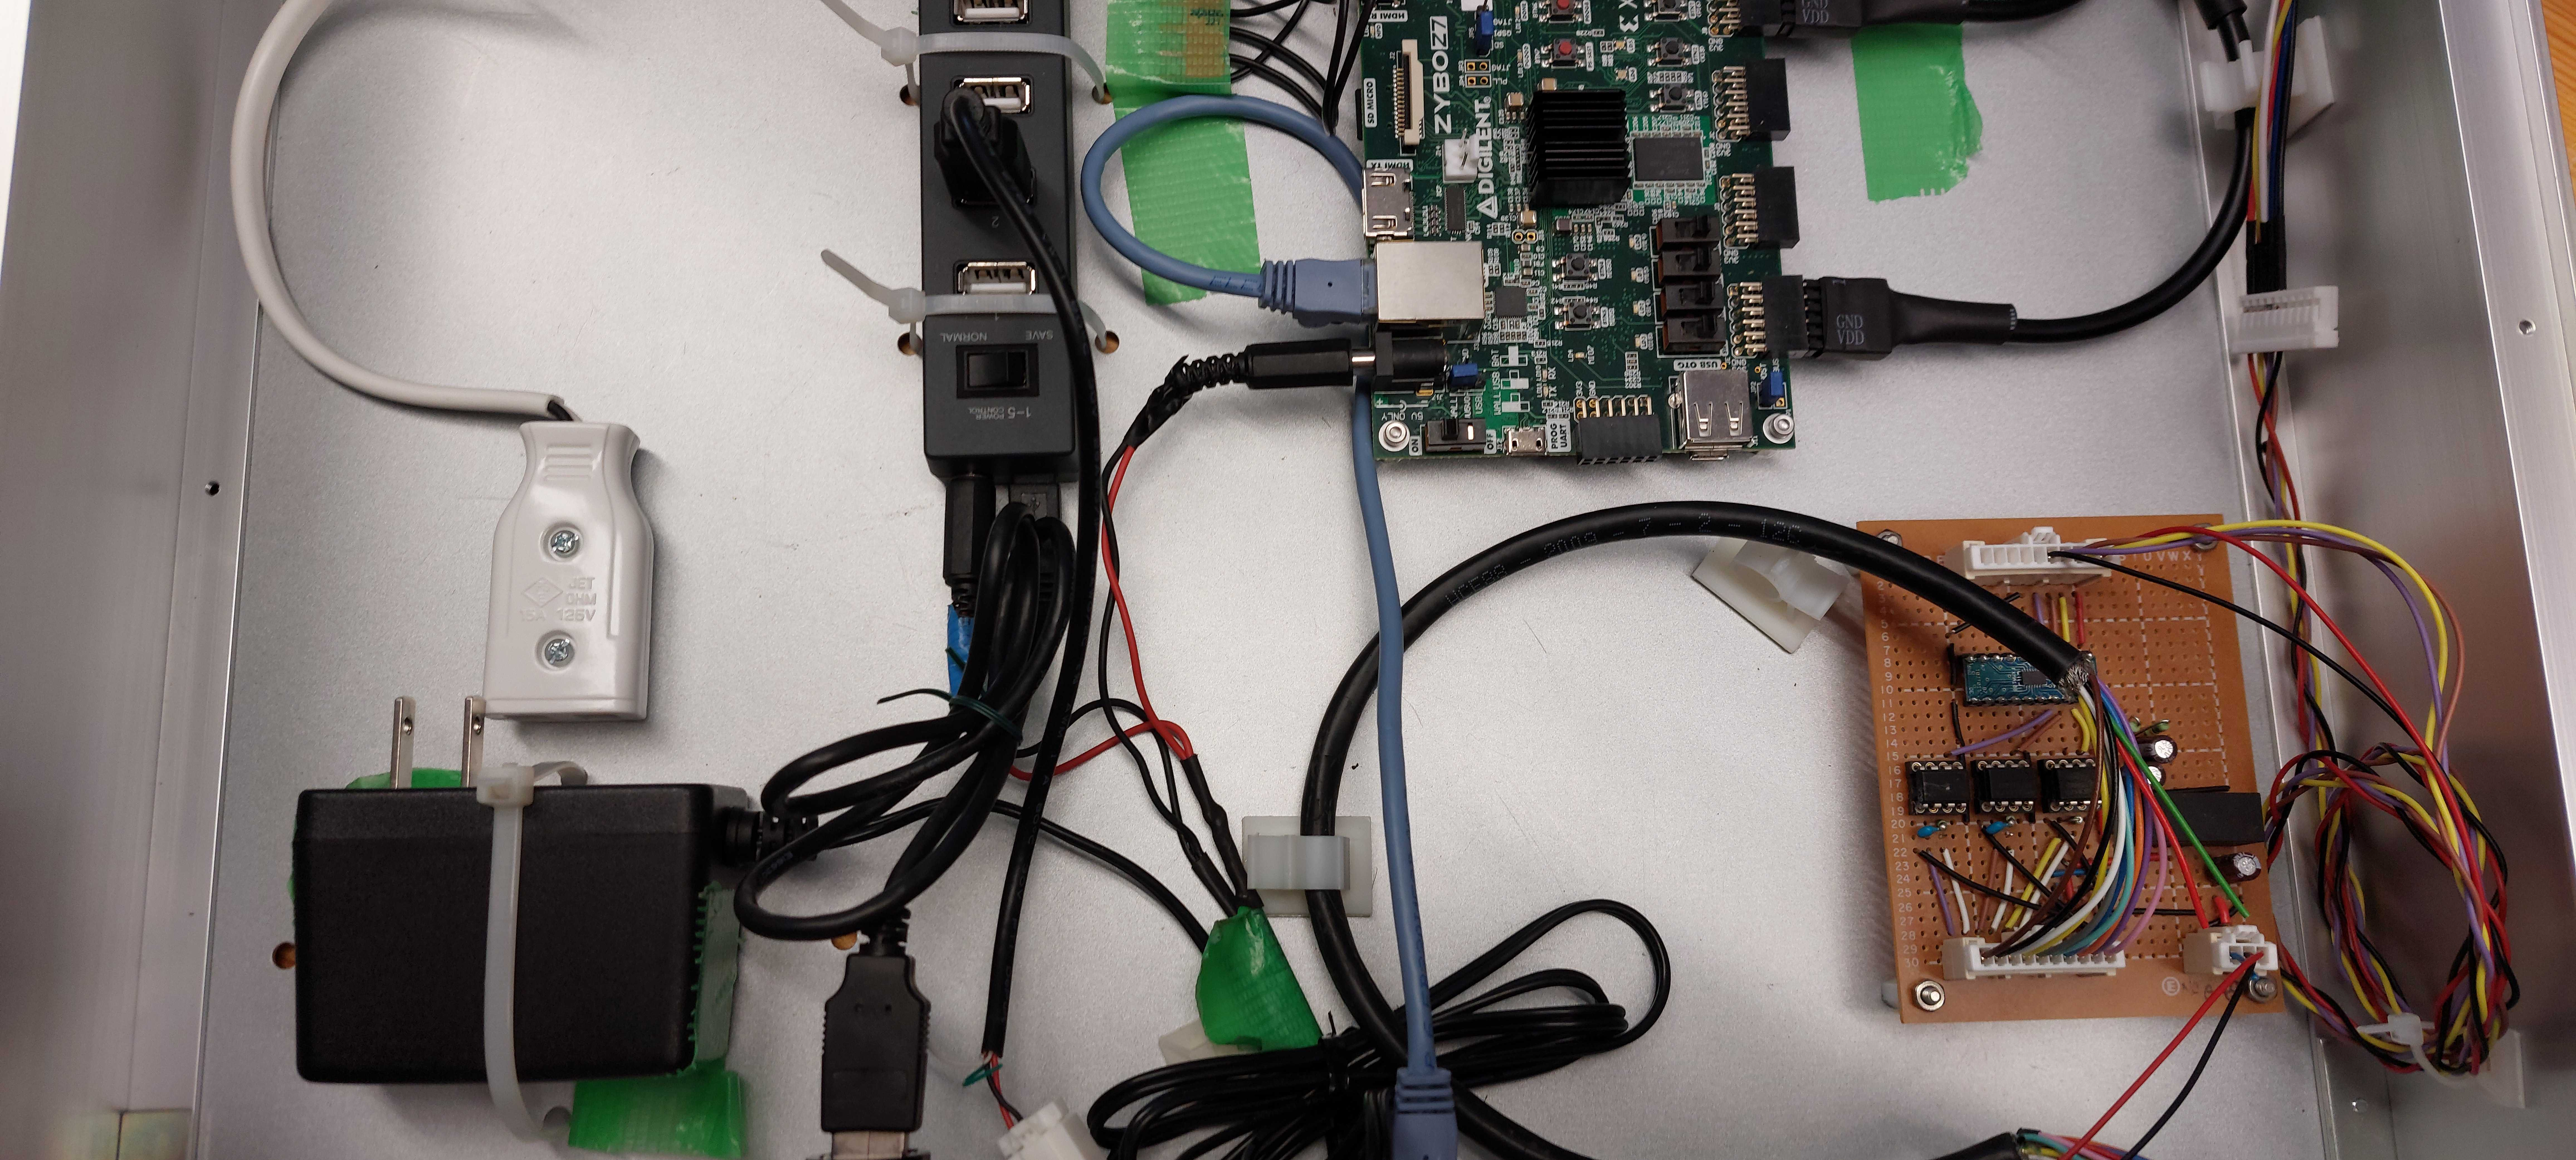
\includegraphics[keepaspectratio, scale=0.02]{4_elDAQ/figs/new_connector_set.jpg}
      \subcaption{配線の変更}
    \end{minipage}
    %---- 2番目の図 --------------------------
    \begin{minipage}[t]{0.45\hsize}
      \centering
      \includegraphics[keepaspectratio, scale=0.02]{4_elDAQ/figs/new_connector_boot.jpg}
      \subcaption{PYNQの再起動}
    \end{minipage}
    %---- 図はここまで ----------------------
  \end{tabular}
  \vspace{5pt}
  \caption{電源供給方法の変更}
  \label{new_connector}
\end{figure}

\subsection{Zynq温度のモニター}
2つ目の要因についても調査し、問題がないことを確認した。ZyboのZynq部分にはヒートシンクが取り付けられており、ある程度の発熱は抑えられるはずだが、消費電力が高いと発熱量が増えてZynqの動作温度の上限($\sim\SI{85}{^{\circ}}$C)を超えることは起きうる。しかし、\ref{power_sup}で見たように新システムの消費電力が大きくなく、稼働中にヒートシンクを手で触っても熱くないため上限を超えるほどの発熱をしていることはまずない。そのことをZynq内の温度モニター機能を用いて確かめた。Zynqには``XADC(Xilinx Analog to Digital Converter) \cite{xadc}''と呼ばれるADCが内蔵されており、供給電圧と温度のモニタリング機能を有している。電圧と温度の値はOSシステムの[ /sys/bus/iio/devices/iio:devices0 ]ディレクトリに出力される。特に温度情報は
\begin{itemize}
  \item in\_temp0\_offset
  \item in\_temp0\_raw
  \item in\_temp0\_scale
\end{itemize}
の3つの値で与えられ、Zynq温度は
\begin{equation}
  \mathrm{T}_{\mathrm{Zynq}}(^{\circ}\mathrm{C}) = (\mathrm{in\_temp0\_raw} + \mathrm{in\_temp0\_offset})\cdot \mathrm{in\_temp0\_scale} / 1000
\end{equation}
で求められる。定期的にZynqの温度を読み出し、値を保存することで温度を確認できるようにした。読み出した温度のプロットを図\ref{temp_zynq}に示す。気温の影響もあるためZynq温度は夏季になると全体的に高くなるが、それでも動作温度の上限である$\SI{85}{^{\circ}}$Cよりも十分低い温度で動作していることが分かる。

%\begin{figure}[h]
  %\begin{tabular}{cc}
    %---- 最初の図 ---------------------------
    %\begin{minipage}[t]{0.45\hsize}
      %\centering
      %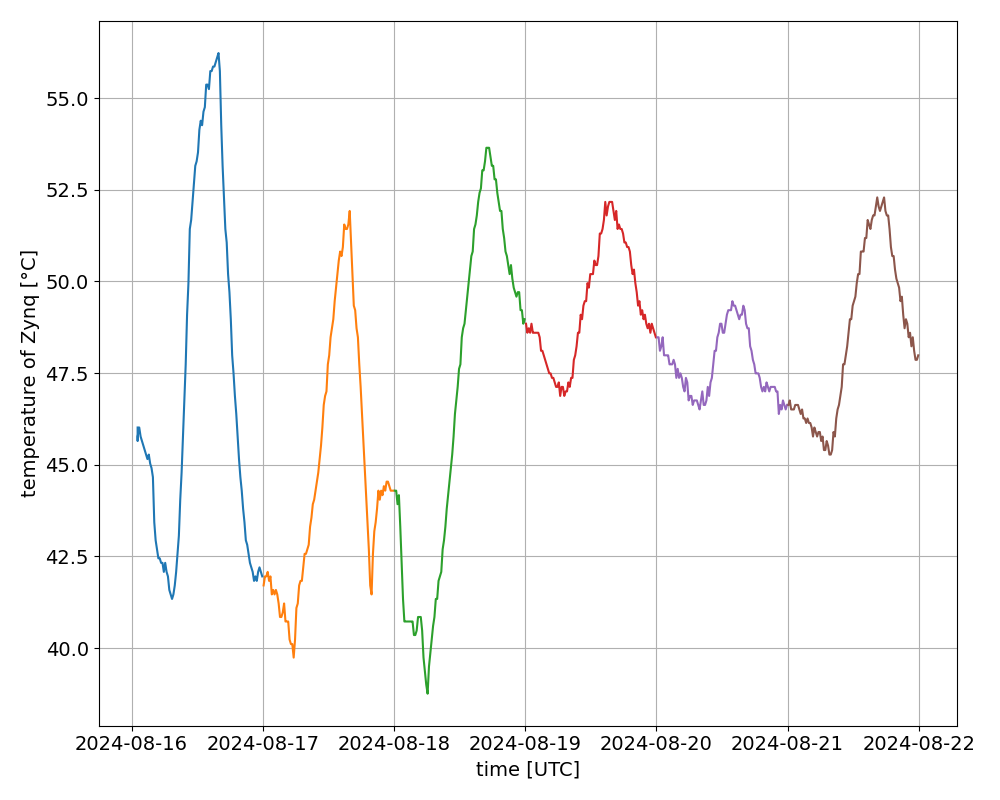
\includegraphics[keepaspectratio, scale=0.25]{4_elDAQ/figs/temp_zynq_202408.png}
      %\subcaption{夏の温度データ}
    %\end{minipage}
    %---- 2番目の図 --------------------------
    %\begin{minipage}[t]{0.45\hsize}
      %\centering
      %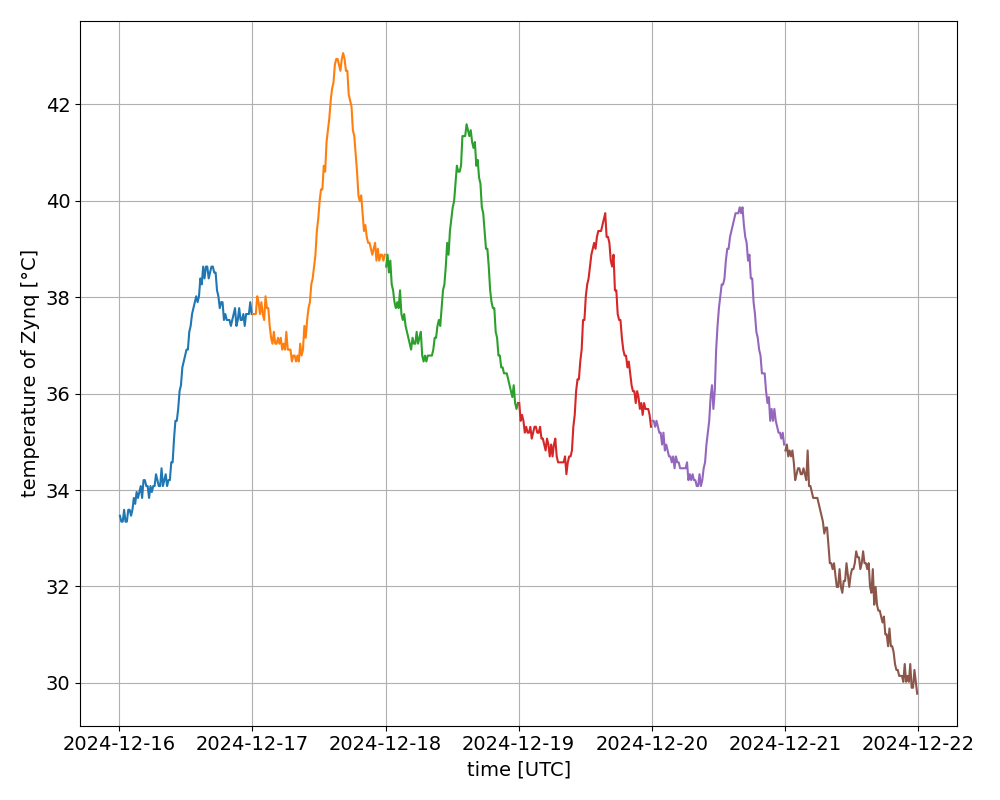
\includegraphics[keepaspectratio, scale=0.25]{4_elDAQ/figs/temp_zynq_202412.png}
      %\subcaption{冬の温度データ}
    %\end{minipage}
    %---- 図はここまで ----------------------
  %\end{tabular}
  %\caption{Zynqの温度モニター}
  %\label{temp_zynq}
%\end{figure}

\begin{figure}[htbp]
  \centering
  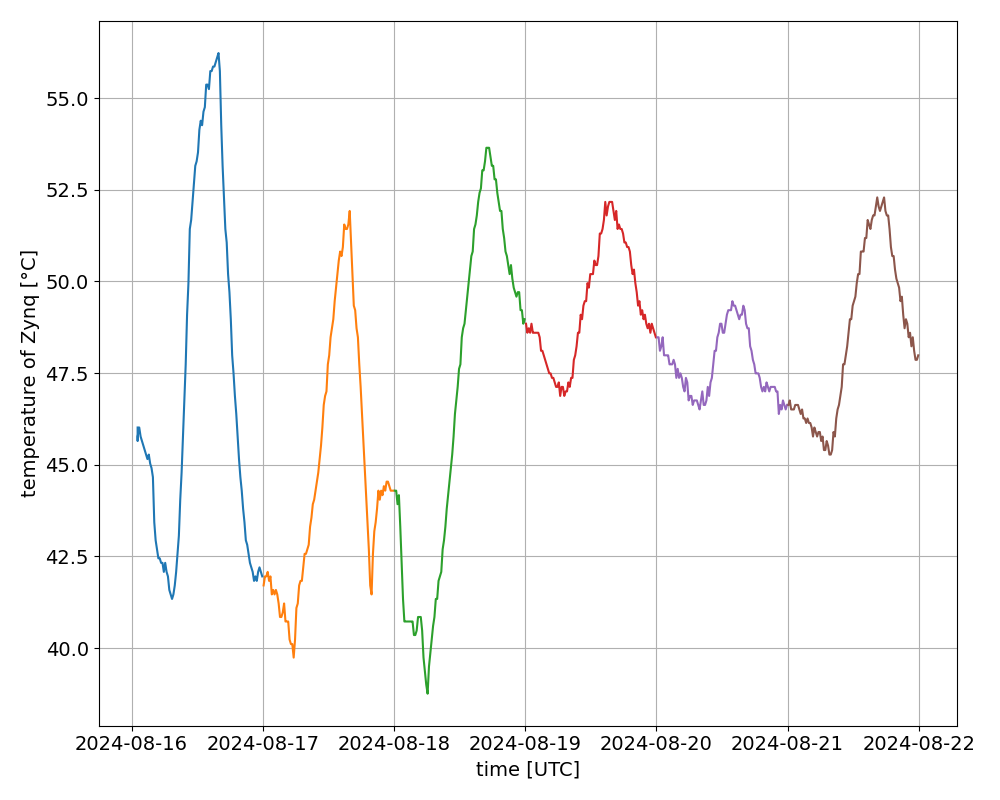
\includegraphics[width=0.9\columnwidth]{4_elDAQ/figs/temp_zynq_202408.png}
  \caption{Zynqの温度モニター。2024/08の6日分のデータをピックアップした。1日の中でも気温の影響を受けてZynqの温度も変動する。そのため、夏季の温度は冬季よりも全体的に高くなる。}
  \label{temp_zynq}
\end{figure}

今後は新しく導入したデータ取得システムの動作状況のモニターを継続して、安定的な運用とメンテナンスを続けていく。

\chapter{焦点面検出器アライメントの較正}
\label{chapter4}

GroundBIRD実験での偏光測定のためには、検出器間での信号の差分を取ることが重要であり、それに伴って望遠鏡のスキャンに対して最適な検出器のアライメントが求められる。この章では検出器アライメントの最適化に向けた改善を行い、観測データからその効果を確認した。

\section{検出器アライメントの問題点}

\subsection{スキャン軸に対する傾きと差分解析}
\label{scan_pair_diff}
まず、GroundBIRDでの解析手法の1つである差分解析と検出器アライメントの関係について述べる。\ref{mkid_design}で示したように、焦点面検出器は異なる偏光方向に感度を持った検出器が交互に配置されている。これらの検出器が検出する信号は空のある点からの放射が望遠鏡内の光学系を経て焦点面へと届いたものである。つまり、焦点面での検出器の配置を空へと射影した時にどう配置されているかが重要になる。各検出器は空のある点を見ており、望遠鏡の方位角回転に伴って同じ仰角の空を回転しながら観測する(図\ref{scan_image})。
\begin{figure}[htbp]
  \centering
  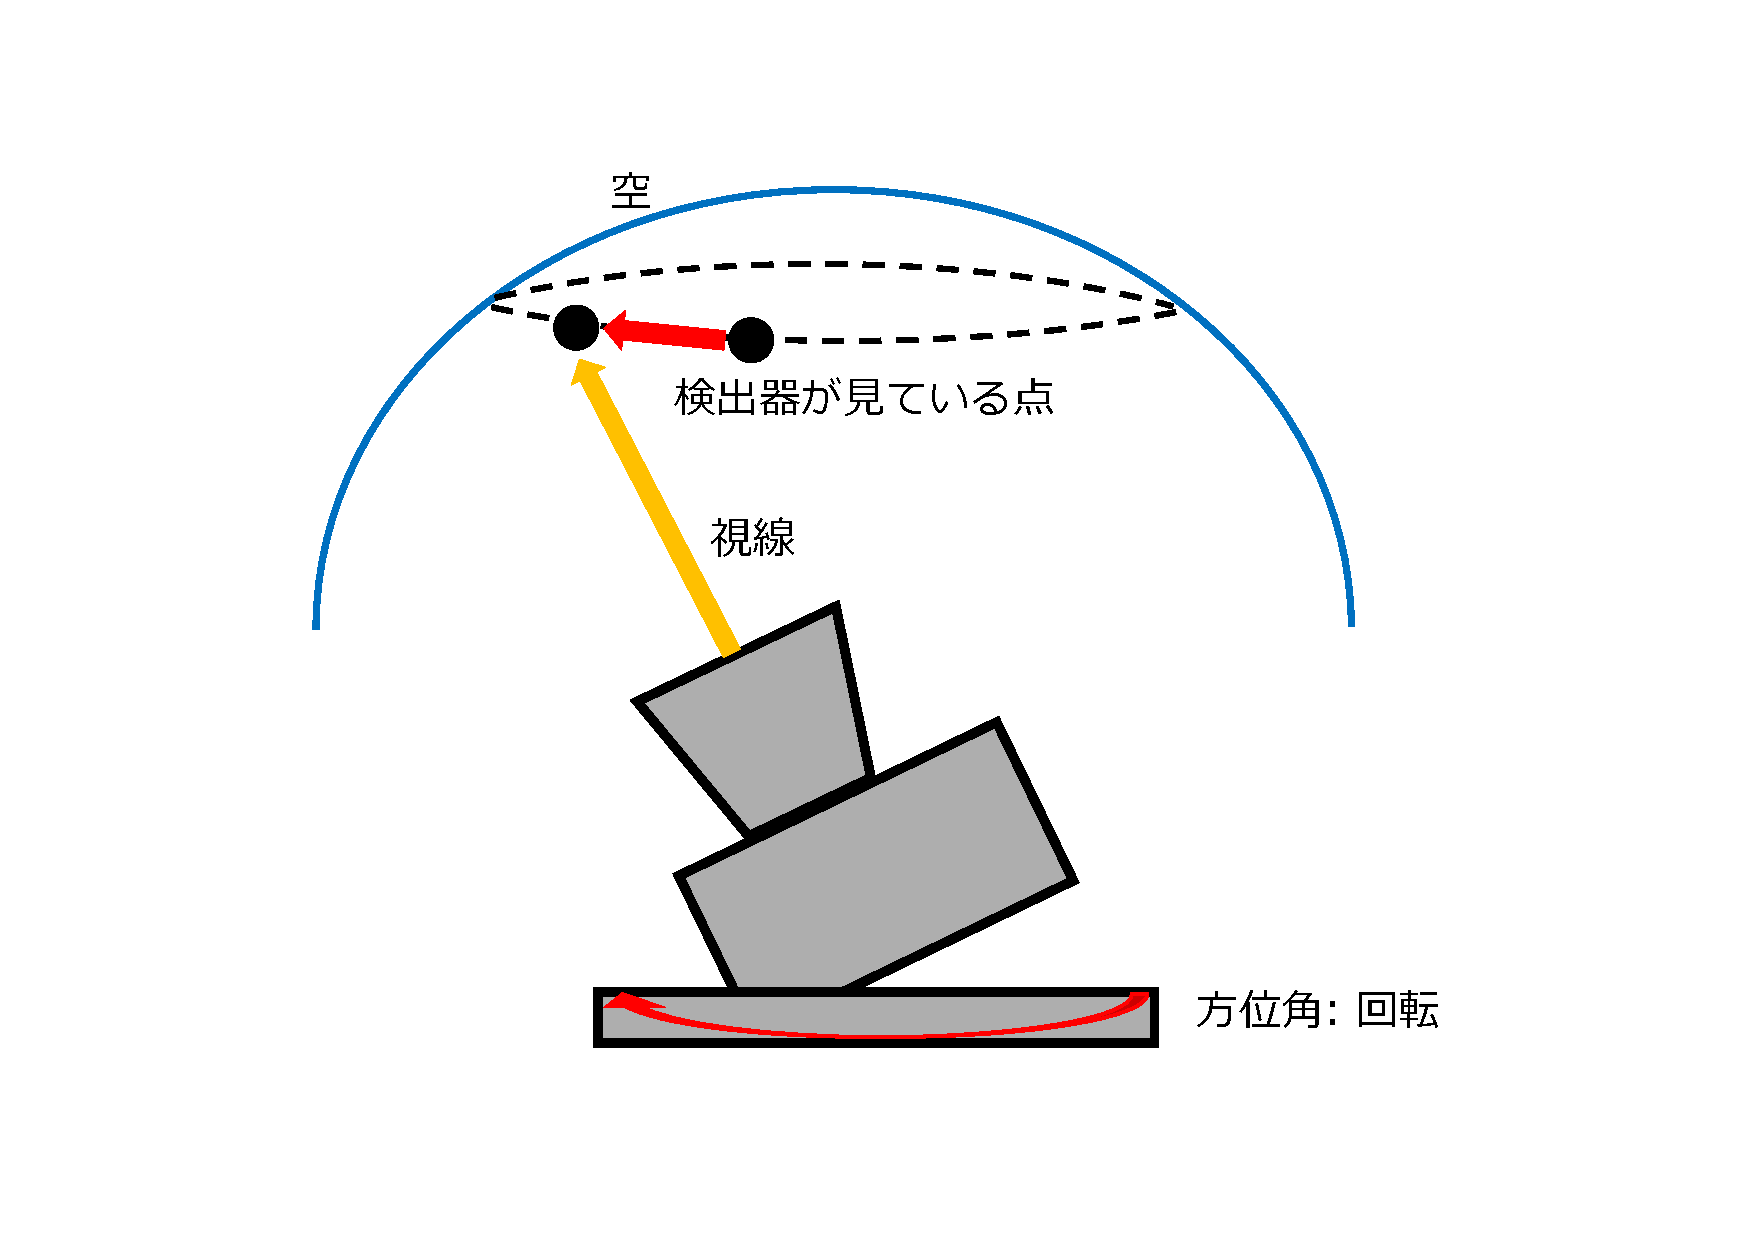
\includegraphics[width=0.6\columnwidth]{5_alignment/figs/scan_image.pdf}
  \caption{検出器が空の領域をスキャンする概要図。ある仰角を高速回転しながらスキャンする。}
  \label{scan_image}
\end{figure}
検出器で観測する信号は大きく(CMB + ノイズ)に分けられる。さらにノイズの中でも寄与が大きい成分に大気放射に由来するノイズがある。このノイズは刻一刻と変動する上に空の領域によっても異なっているため、高速回転によるスキャンで異なる検出器が同じ空の領域をスキャンすることで抑制できる。具体的には、異なる偏光方向に感度のある検出器が同じ仰角の空をスキャンする時、もう一方の検出器は片方の検出器が観測した空の領域をわずかな時間差で観測することができる。つまり、スキャンの間に大気の情報は変動せず観測される大気由来のノイズも変動しないことになる。そのため、検出器間で信号の差分をとることで、大気ノイズは共通していると考えれば取り除くことができ、偏光成分のみを残すことができる。しかし、検出器の配置がずれていて検出器間でスキャンする空の領域が異なる場合、大気の情報も異なり、差分をとっても大気ノイズを取り除くことができない(図\ref{scan_axis})。
\begin{figure}[htbp]
  \centering
  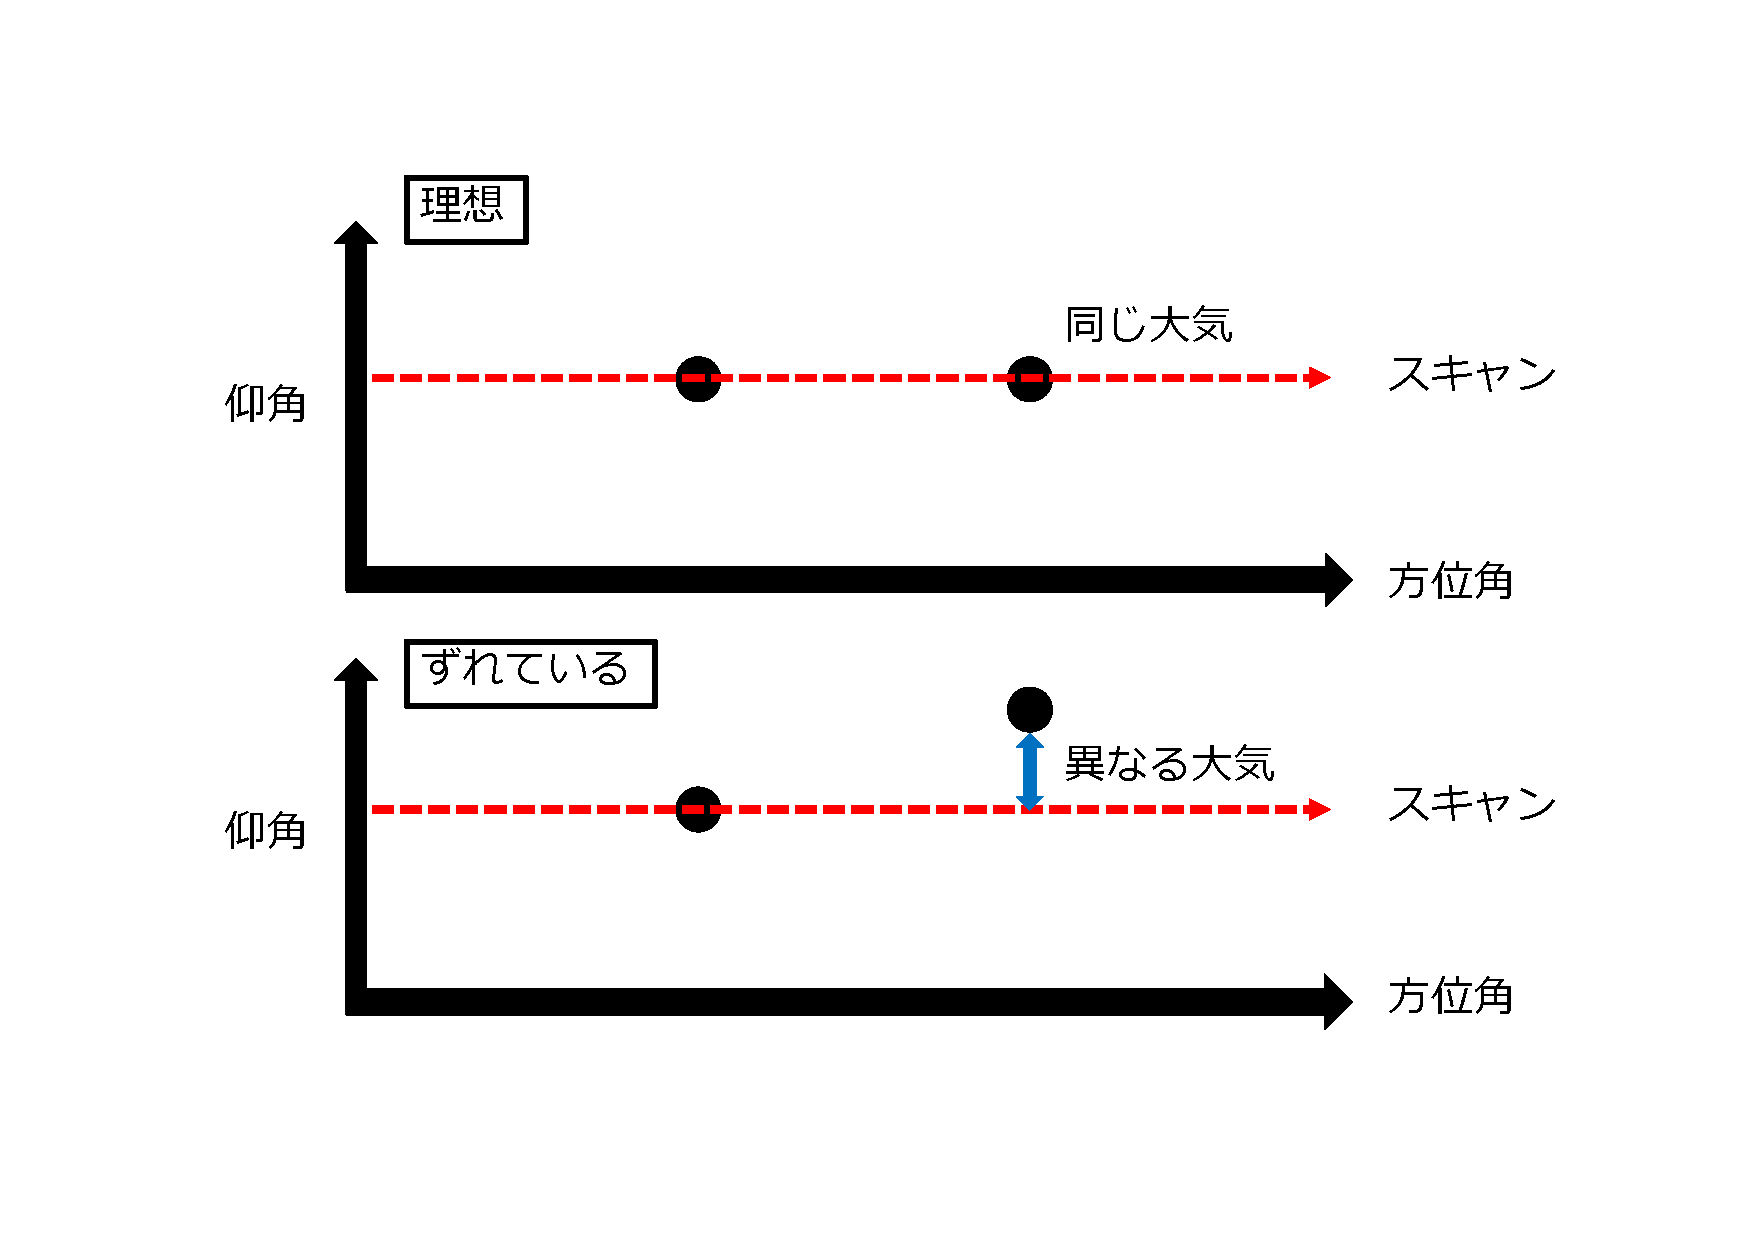
\includegraphics[width=0.7\columnwidth]{5_alignment/figs/scan_axis.pdf}
  \caption{空での理想的な検出器の配置とずれている場合の配置との比較。スキャン軸(方位角軸)に沿って検出器が並んでいないと観測する大気が検出器ごとに異なる。}
  \label{scan_axis}
\end{figure}

以上から空での理想的な検出器の配置は``複数の検出器がスキャン軸に沿って並んでいる''ことである。

しかし、観測データから理想的な検出器の配置からずれていることが示唆されていた。また、そのずれはスキャン軸に対して無視できないほどに有意な角度で傾いているものだと考えられていたが十分な検証と較正(実際に何度傾いているのか、傾きがあることでどれ程大気ノイズの影響が残ってしまうのか、など)がされていなかった。検出器アライメントの問題を改善し、GroundBIRDが持つ観測性能を最大限に引き出すことは質の良いデータを取得するためには不可欠である。

\subsection{要求される理想的なアライメント}

GroundBIRDにおける理想的な検出器の配置について詳細を見ていく。焦点面検出器は図\ref{full_array_picture}のように7つの検出器アレイが平面的に取り付けられているが、この検出器が観測する領域は平面のまま空に射影される訳ではない。観測する空の点は天球面上に張り付いた点と考えられるため、球面として射影される。焦点面検出器が平面を見るときと空を見る時での理想的な配置の違いを図\ref{distortion_pos}に示す。実際には球面から来る歪みの影響を受けた配置として空を観測することになり、望遠鏡の視線中心(\SI{220}{GHz}アレイ)ではほぼ平面だが、中心から離れた検出器は歪みの影響が出る。歪みを考慮した上で複数の検出器をスキャン軸に沿って並べることは焦点面の設計上難しい。また、高周波になるほど大気放射の寄与が大きくなる\cite{atmos_radiation}ことから、本論文では歪みの影響が少なく、大気放射の寄与も大きい中心の\SI{220}{GHz}アレイに対して配置がスキャン軸に沿って並んでいること、中心以外の\SI{145}{GHz}アレイに対して配置が仰角軸に対称であることを理想的なアライメントとする。
\begin{figure}[htbp]
  \centering
  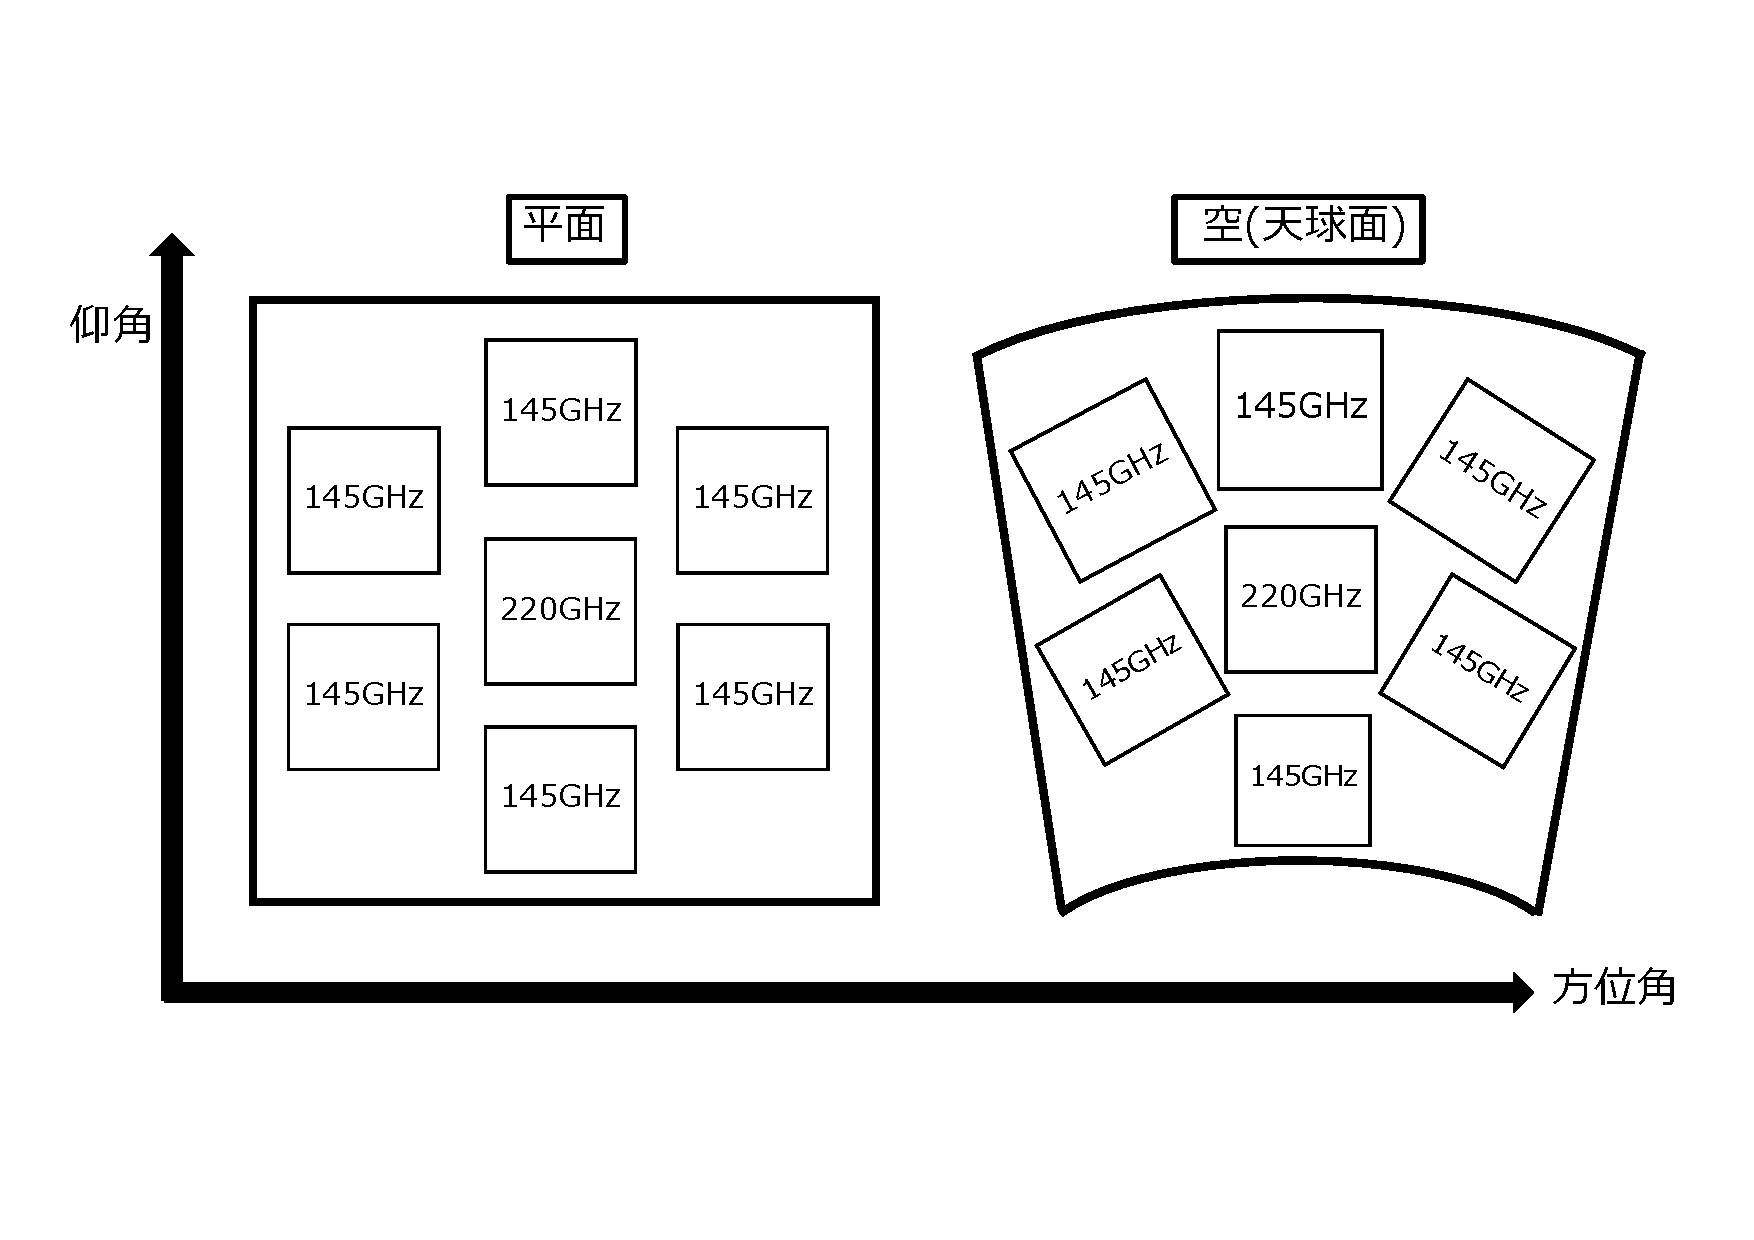
\includegraphics[width=0.8\columnwidth]{5_alignment/figs/distortion_pos2.pdf}
  \caption{平面と空(天球面)での理想的な検出器配置の違い。}
  \label{distortion_pos}
\end{figure}
\subsection{視線軸方向まわりの回転による較正}

スキャン軸に対して傾いた焦点面検出器を理想とする配置にするためには、検出器の視線を回転させてスキャン軸に並べれば良いことになる。また、焦点面検出器は望遠鏡内部で固定されているため望遠鏡全体の視線を回転することに対応する。つまり、望遠鏡のビーム中心を望遠鏡の視線方向とし、視線方向軸周りに適当な角度回転させることで各検出器の視線を回転させる(図\ref{boresight_axis})。
\begin{figure}[htbp]
  \centering
  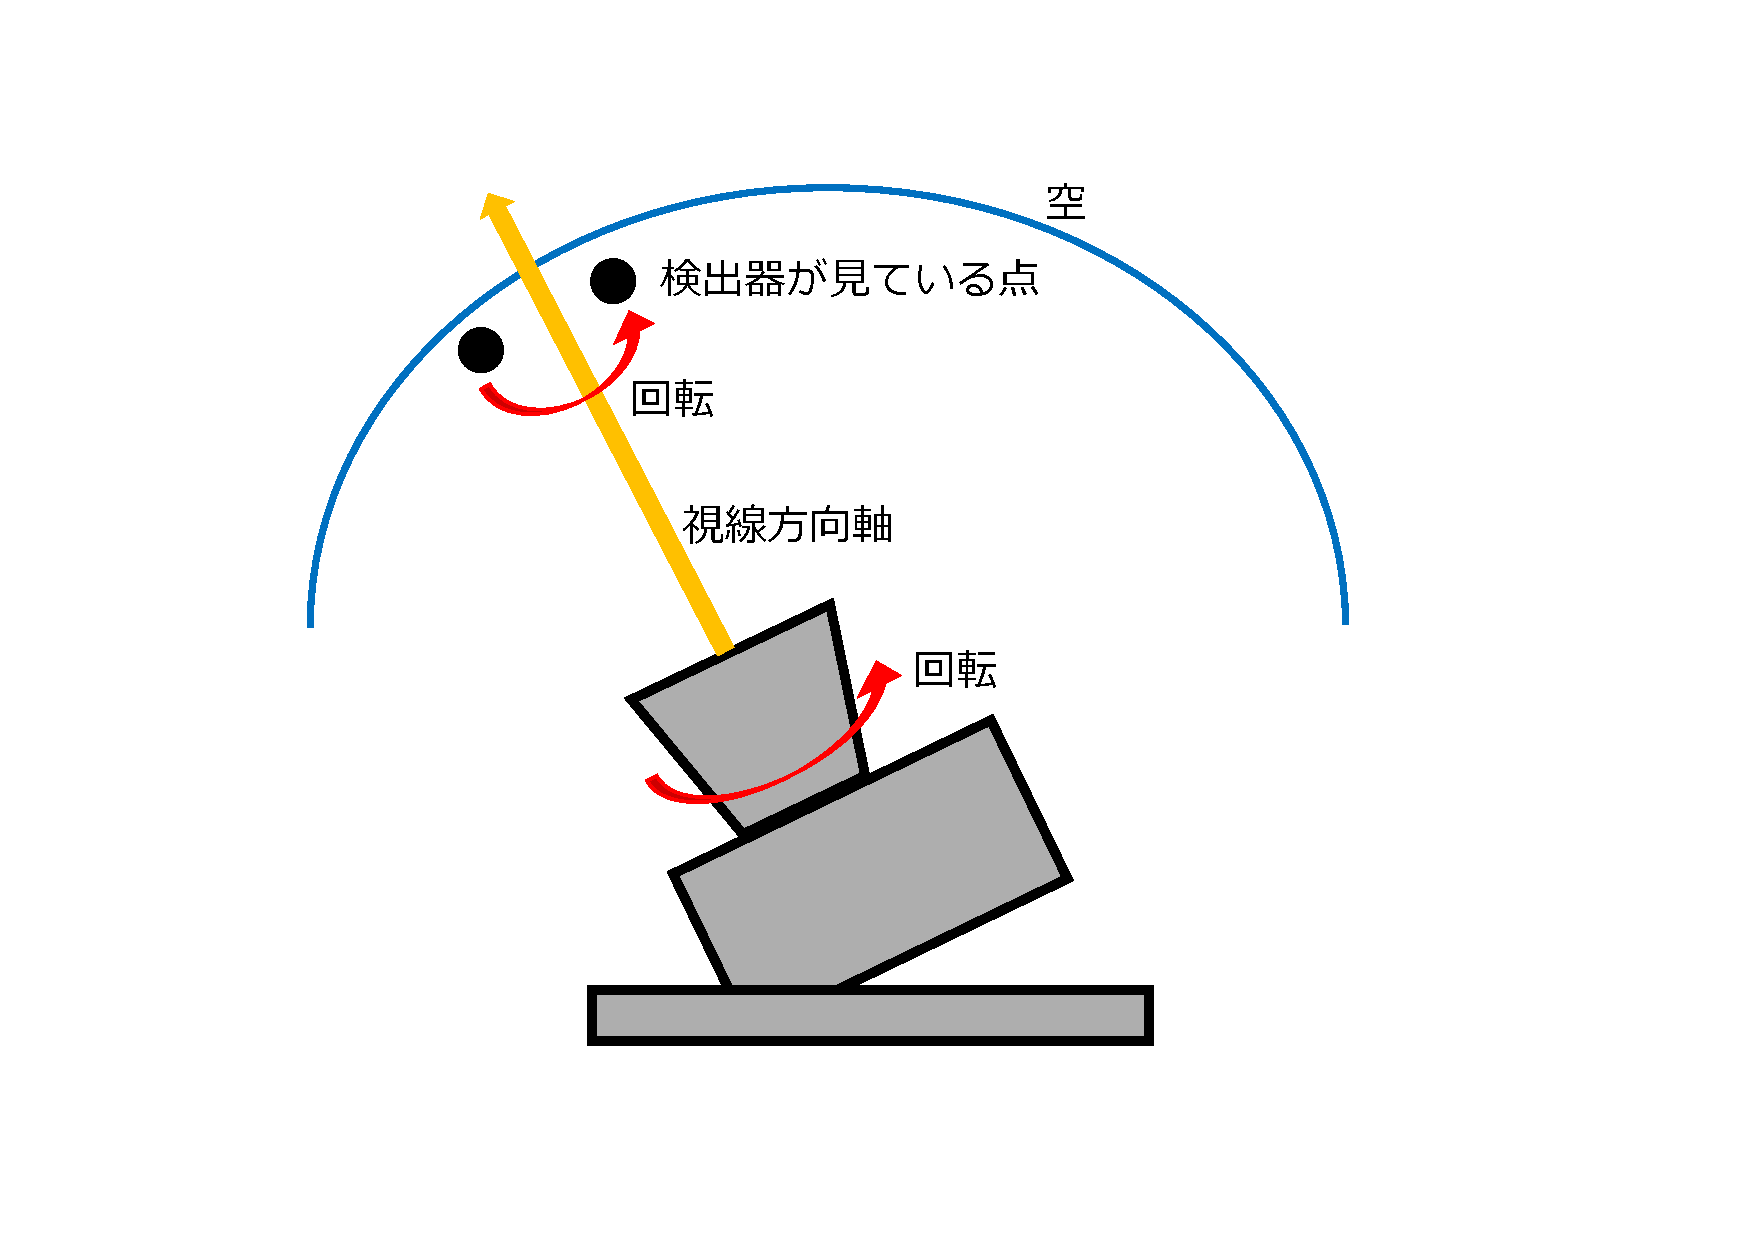
\includegraphics[width=0.8\columnwidth]{5_alignment/figs/boresight_axis.pdf}
  \caption{望遠鏡の視線方向軸と軸周りの回転。検出器の見ている点(視線)も回転する。}
  \label{boresight_axis}
\end{figure}
%検出器の配置がビームの中心に対して傾いている場合、視線方向軸の周りに望遠鏡を適当な角度回転させることで配置をスキャン軸に沿って並ばせることが可能になる。

そのため、理想的なアライメントにするための回転角を見積もる必要がある。回転角を求めるには各検出器の見ている点を知る必要があり、天体の観測データを解析することで算出できる(天体の運動が分かっているので検出器データと角度データから各検出器の視線情報を求められる)。

\section{月を用いた回転角の算出}

\subsection{月を用いた理由}

GroundBIRDで観測できる天体として月や惑星(木星、金星)が挙げられる。しかし、月と惑星ではデータの性質は大きく異なり、それぞれ観測上の長所と短所が存在する。月データと惑星データの特徴を表\ref{moon_vs_planet}に示す。
\begin{table}[htbp]
%\begin{threeparttable}[htbp]
  \centering
  \caption{月データと惑星データの比較\cite{sueno_doctor}}
  \vspace{3mm}
  \begin{tabular}{ccc} \hline
    & 月 & 惑星 \\ \hline
    長所 &
    \begin{tabular}{c}
    S/N比が高い \\ (1度の観測で十分な信号を得られる)
    \end{tabular} &
    \begin{tabular}{c}
    点源として扱える \\ (角直径がビーム幅に比べて十分小さい)
    \end{tabular} \\ \hline
    短所 &
    \begin{tabular}{c}
    点源として扱えない \\ (輝度温度の非一様性が生じる)
    \end{tabular} &
    \begin{tabular}{c}
    S/N比が小さい \\ (データを蓄積しないとノイズに埋もれる)
    \end{tabular} \\ \hline
  \end{tabular}
  \label{moon_vs_planet}
\end{table}
%\end{threeparttable}
検出器の視線情報を得るには点源として扱え、正確に点として求められる惑星が適しているが、\ref{jupiter_ana}で見るように点源で最も明るい木星の観測データでもノイズの影響をかなり受けてしまう。そのため、データを蓄積するか、PWVや湿度が十分低く観測条件が整った観測データを使用する必要がある。一方、月は高いS/N比により1度の観測データで十分な信号を得られ、データを蓄積することによるノイズが加わることなく解析ができる。点源として扱えないことによる誤差はあるものの\footnote{月の輝度温度は月齢によって大きく変動し、月齢を$\phi$~[deg]、波長$\lambda$に対して$\delta=0.3\cdot\lambda$~[mm]とすると、輝度温度$\overline{T_{\mathrm{MOON}}}$は
\begin{equation}
  \overline{T_{\mathrm{MOON}}}=225\Bigl\{1+\frac{0.77}{\sqrt{1+2\delta+2\delta^{2}}}\cos\bigl(\phi-\arctan\frac{\delta}{1+\delta}\bigr)\Bigr\}
\end{equation}
と経験的に表せる\cite{dennpa_tennmonn}。}、高いS/N比がそれをカバーできると考えたため、月のデータを選択した。

\subsection{位相としての検出器TOD}
GroundBIRDにおける観測データは\ref{MKID}で述べた超伝導検出器MKIDの共振状態の変化を入射信号の大きさとして\SI{1}{kSPS}で取得するTODのことである。共振状態の変化とはすなわち共振周波数の変化であるが、これを読み出しRF信号の透過率の変化として測定する。透過率は散乱行列要素の$S_{21}$で表す。MKIDの$S_{21}$は共振の鋭さを表す$Q_{r}$, $Q_{c}$を用いて
\begin{equation}
  |S_{21}-x_{c}| = \frac{Q_{r}}{2Q_{c}} \bigl(x_{c} = 1-\frac{Q_{r}}{2Q_{c}}\bigr)
\end{equation}
で得られ\cite{muto}、$S_{21}$の軌跡が円状になることが分かる。この円は``共振円''と呼ばれる。共振円と$S_{21}$の例を図\ref{res_circ}に示す。
\begin{figure}[htbp]
  \centering
  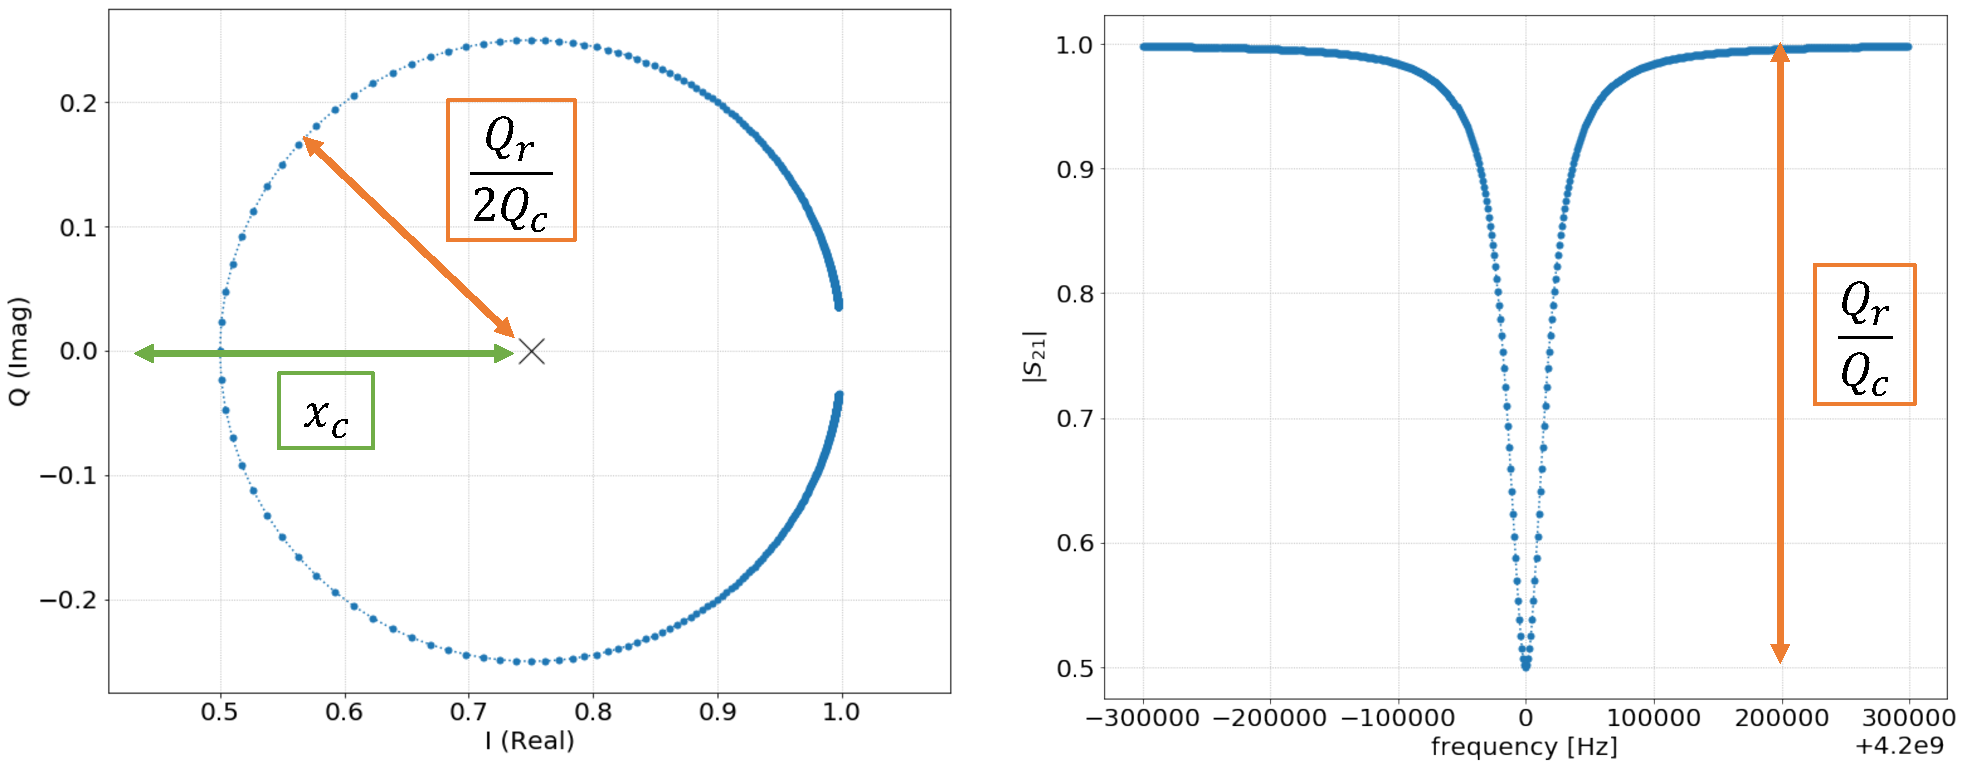
\includegraphics[width=1.0\columnwidth]{5_alignment/figs/iq_amp.pdf}
  \caption{共振円と共振周波数付近での透過率。\cite{sueno_master}より引用。}
  \label{res_circ}
\end{figure}
共振周波数の周りで透過率が鋭いピークを持つことが分かる。共振円を動く$S_{21}$の振幅$A$と位相$\theta$を
\begin{equation}
  A = \frac{|S_{21}|- x_{c}}{1-x_{c}}
\end{equation}
\begin{equation}
  \tan\theta = \frac{\mathrm{Im}(S_{21})}{x_{c}- \mathrm{Re}(S_{21})}
\end{equation}
と定義する。これらの値は共振周波数の変化に対して敏感であるため、振幅の変化($\delta A$)と位相の変化($\delta\theta$)によって入射信号の大きさを読み出せる。入射信号によって振幅と位相が変化する例を図\ref{amp_and_phase}に示す。
\begin{figure}[htbp]
  \centering
  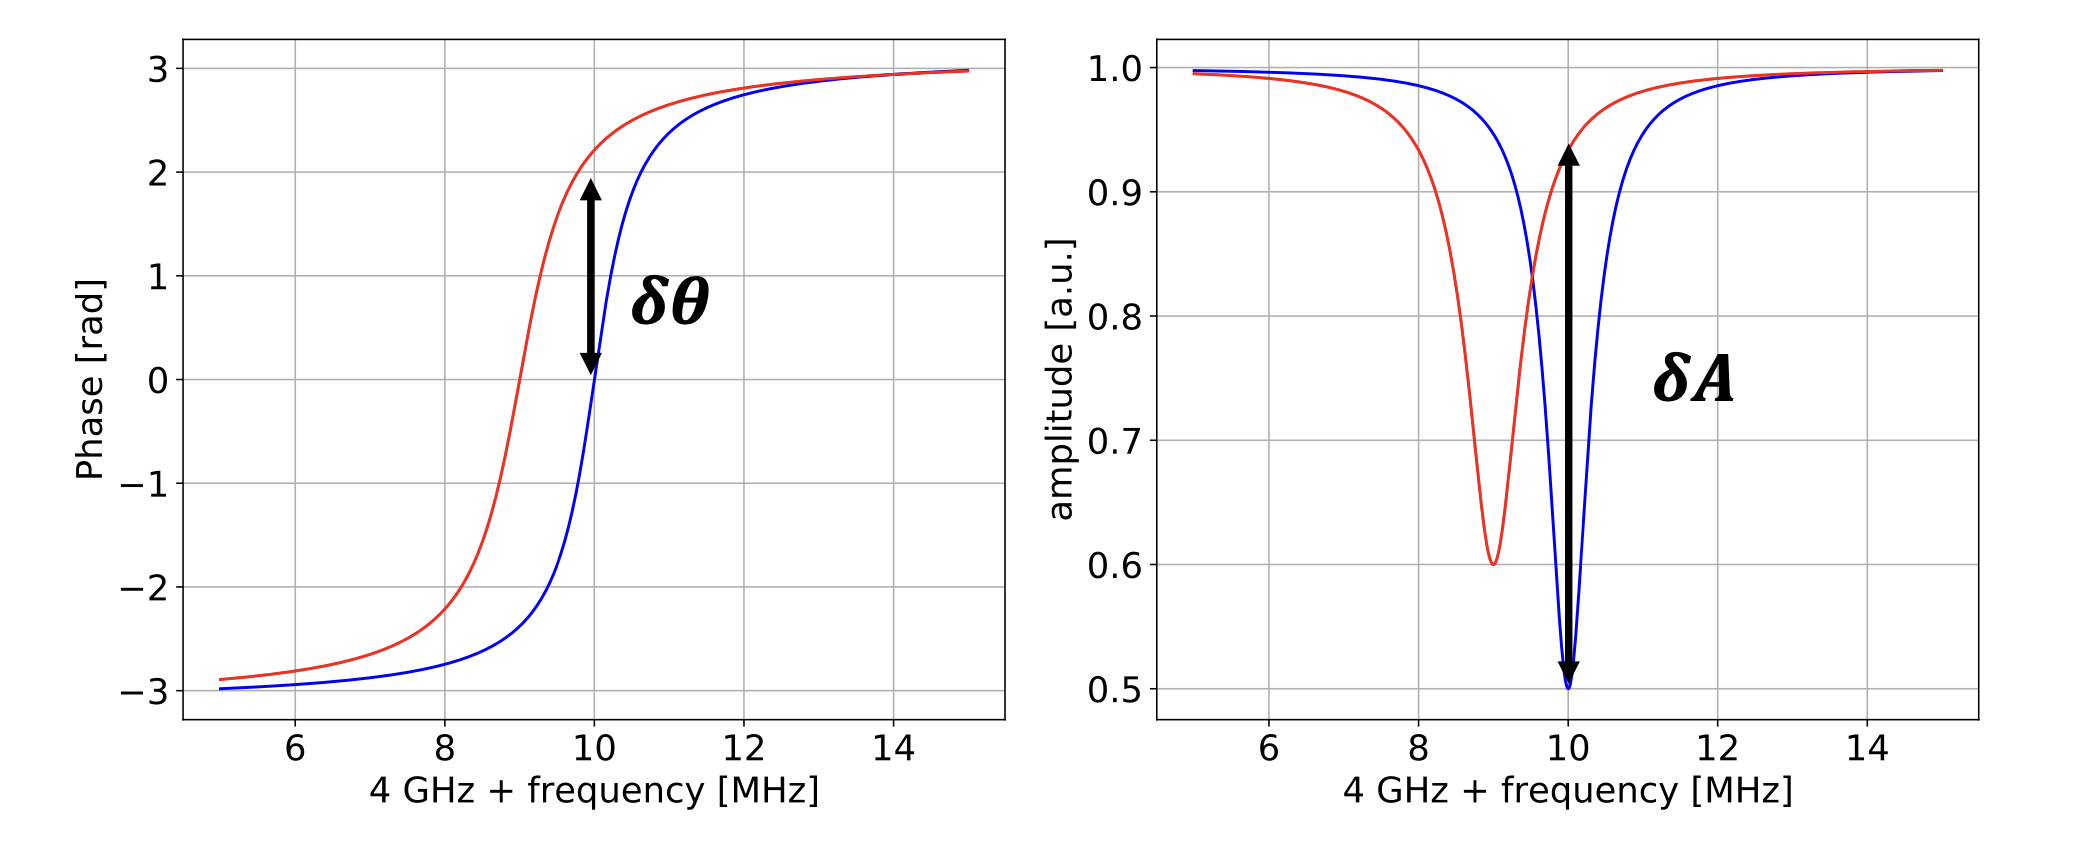
\includegraphics[width=1.0\columnwidth]{5_alignment/figs/amp_and_phase.png}
  \caption{共振周波数付近での$S_{21}$の振幅と位相の変化。\cite{sueno_doctor}より引用。}
  \label{amp_and_phase}
\end{figure}

実際のTOD取得時には図\ref{amp_and_phase}のように各MKIDで固定した共振周波数で測定を行う。そのため、TOD取得前に各MKIDの共振周波数を知る必要がある。また、共振周波数は観測条件によって変動するため、一定の値をとらない。そのため、1観測を1時間で区切っており、1観測ごとにTOD取得前に共振周波数を求めている(その間も望遠鏡は連続的に稼働している)。共振周波数を知るために
\begin{enumerate}
  \item 周波数スイープ
  \item フィッティング
\end{enumerate}
の手順で測定をする。周波数スイープとは、読み出し用のRF信号の周波数を少しずつ変えながら測定をする手法である。測定量はRFの透過率で、スイープで測定されたデータを透過率の関数でフィットすることで共振周波数を求める。フィット関数は$S_{21}$に補正項を入れたもので
\begin{equation}
  T_{21}(f) = a_{0}~\mathrm{exp}(-2\pi if\tau_{0})\biggl(1-\frac{Q_{r}/Q_{c}e^{i\phi}}{1+2iQ_{r}(f-f_{r})/f_{r}}\biggr)
\end{equation}
で表される\cite{sueno_master}。ここで、$a_{0}$, $\tau_{0}$は読み出し回路による振幅の減衰と位相のずれを表す。$e^{i\phi}$はCカップリングでのインピーダンスを補正する項である。このフィットで共振周波数$f_{r}$と共振の鋭さを表す$Q_{r}$, $Q_{c}$を得られる。得られた$f_{r}$にRF周波数を固定し、TODを取得する。TODでの測定量は$T_{21}$であり、補正項の効果を差し引くことで$S_{21}$としての振幅$A$と位相$\theta$を取得できる。
%\begin{equation}
  %|S_{21}-x_{c}| = \frac{Q_{r}}{2Q_{c}} \bigl(x_{c} = 1-\frac{Q_{r}}{2Q_{c}}\bigr)
%\end{equation}
%で得られ\cite{muto}、$S_{21}$の軌跡が円状になることが分かる。この円は``共振円''と呼ばれる。共振円と$S_{21}$の例を図\ref{res_circ}に示す。
%\begin{figure}[htbp]
  %\centering
  %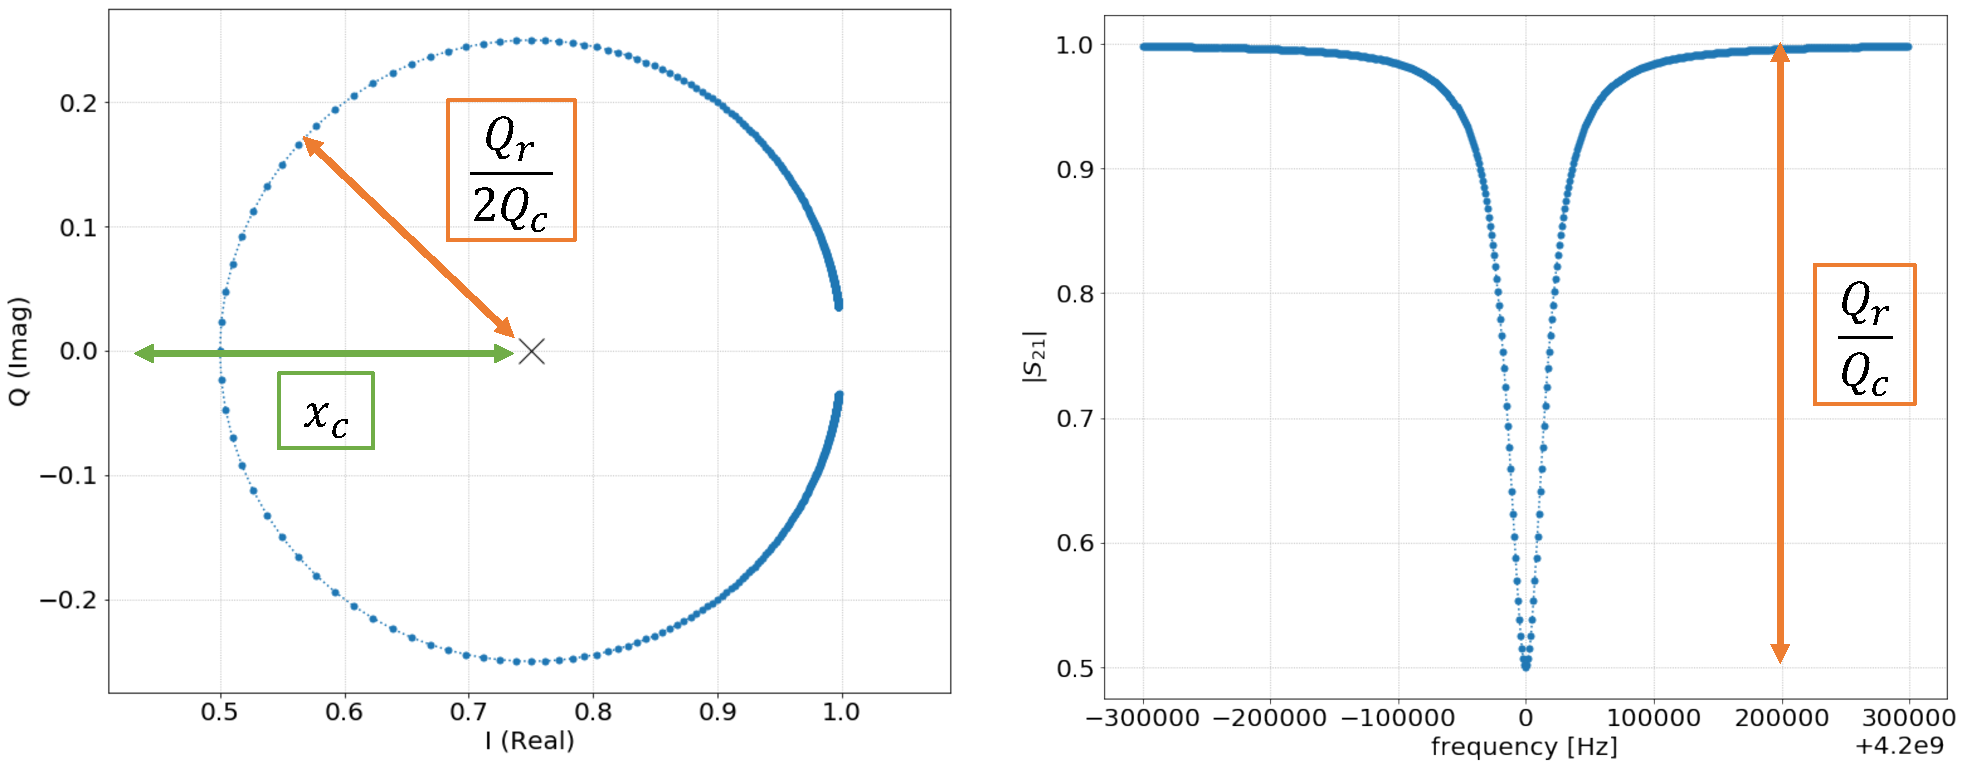
\includegraphics[width=0.9\columnwidth]{5_alignment/figs/iq_amp.pdf}
  %\caption{共振円と共振周波数付近での透過率。\cite{sueno_master}より引用。}
  %\label{res_circ}
%\end{figure}
%共振周波数の周りで透過率が鋭いピークを持つことが分かる。共振円を動く$S_{21}$の振幅$A$と位相$\theta$を
%\begin{equation}
  %A = \frac{|S_{21}|- x_{c}}{1-x_{c}}
%\end{equation}
%\begin{equation}
  %\tan\theta = \frac{\mathrm{Im}(S_{21})}{x_{c}- \mathrm{Re}(S_{21})}
%\end{equation}
%と定義する。これらの値は共振周波数の変化に対して敏感であるため、振幅の変化($\delta A$)と位相の変化($\delta\theta$)を測定することで入射信号の大きさを読み出せる。入射信号によって振幅と位相が変化する例を図\ref{amp_and_phase}に示す。
%\begin{figure}[htbp]
  %\centering
  %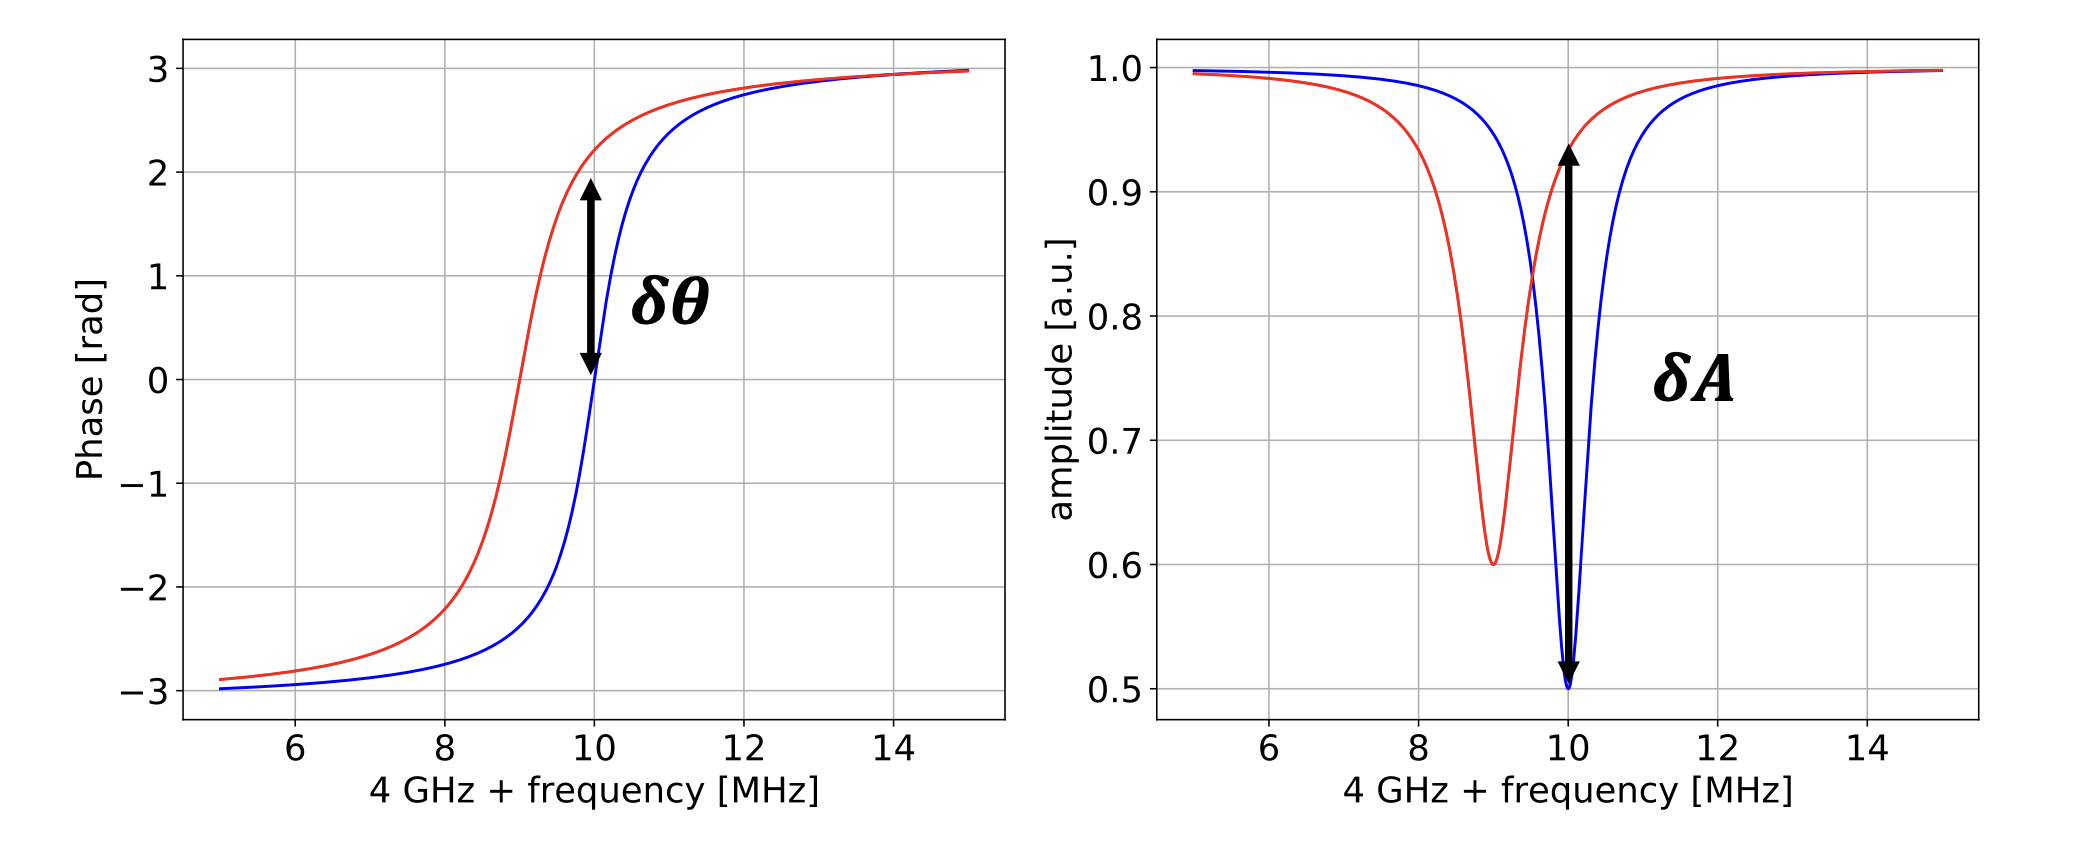
\includegraphics[width=1.0\columnwidth]{5_alignment/figs/amp_and_phase.png}
  %\caption{共振周波数付近での$S_{21}$の振幅と位相の変化。\cite{sueno_doctor}より引用。}
  %\label{amp_and_phase}
%\end{figure}
本論文ではより応答性の高い位相をTODとして使用する。また、非線形効果を補正したものを最終的に使用する位相TODとした。非線形効果の補正は位相の応答($\theta_{\mathrm{res}}$)に対して以下の式\cite{sueno_doctor}を用いた。
\begin{equation}
  \theta = 2\tan(\theta_{\mathrm{res}}/2)
\end{equation}
最終的に使用する位相TODの例(1観測)を図\ref{raw_phase}に示す。
\begin{figure}[htbp]
  \centering
  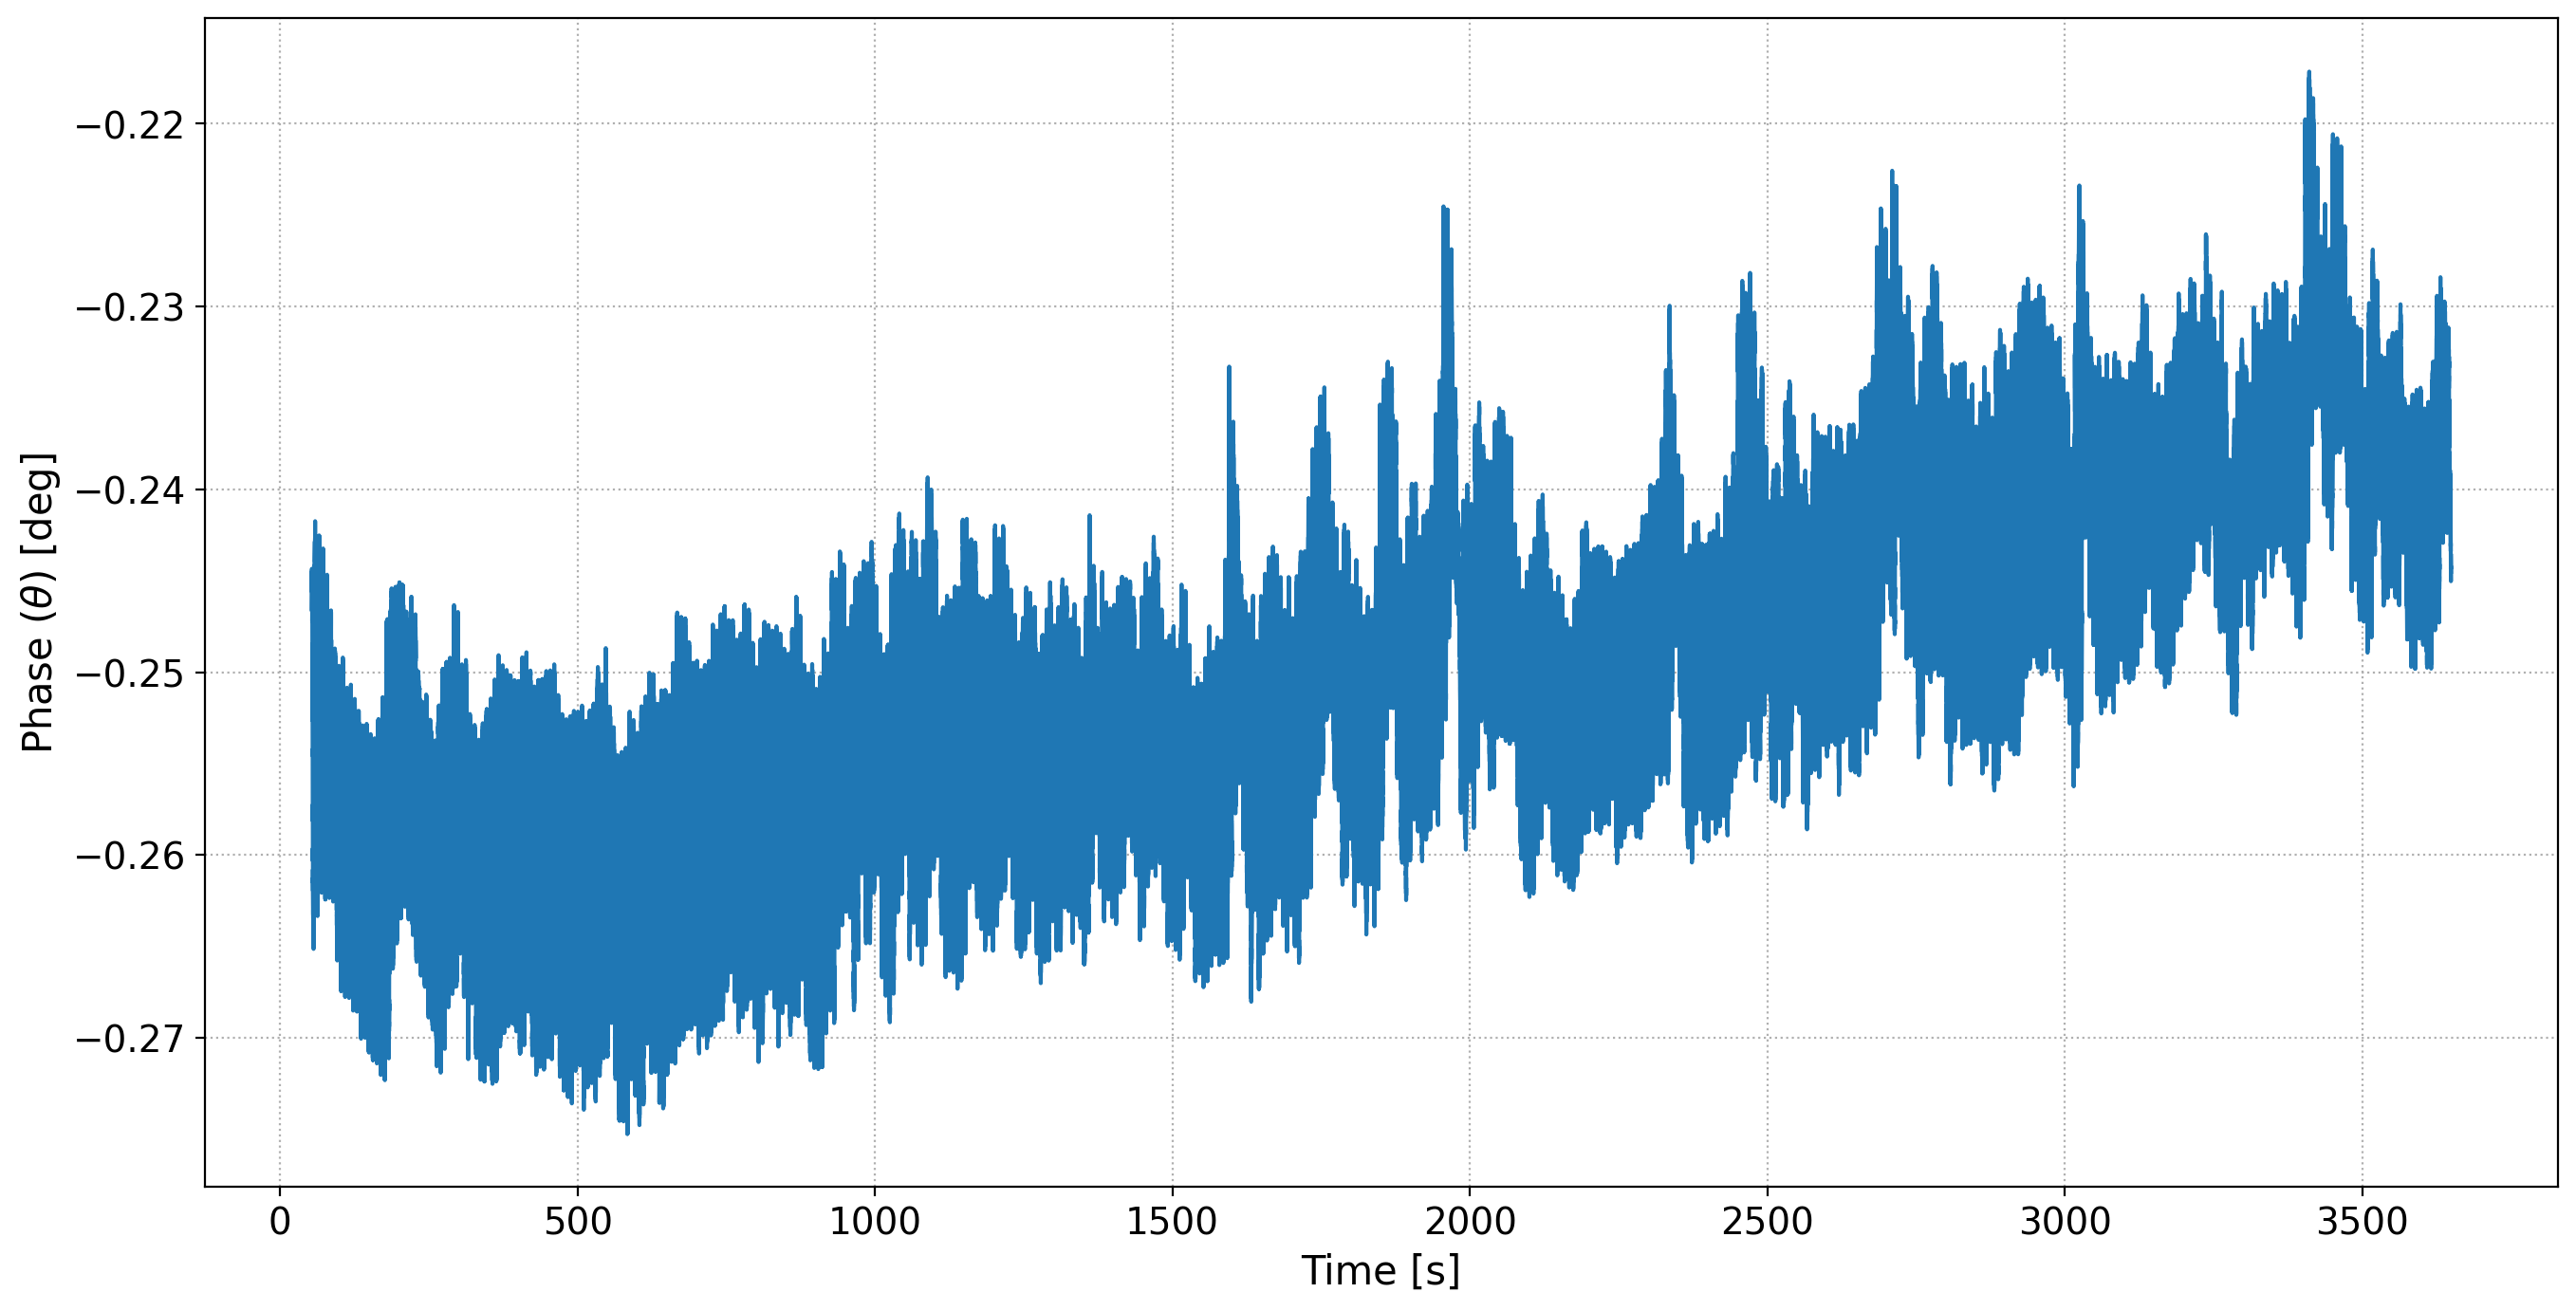
\includegraphics[width=0.9\columnwidth]{5_alignment/figs/raw_phase_deg.png}
  \caption{非線形効果を加えた位相TOD。本論文ではこのTODを用いる。}
  \label{raw_phase}
\end{figure}

\subsection{必要な回転角}
\label{angle_calculation}
月の信号は大きく1観測のTODで鮮明なマップを得ることができる。月を観測した時(2023/12/02、1時間)の位相TODを図\ref{6550_kid0_phase}に示す。
\begin{figure}[htbp]
  \centering
  \includegraphics[width=0.85\columnwidth]{5_alignment/figs/6550_kid0_phase.png}
  \caption{月観測時のTOD。月の中心を観測した時にピークを取る。}
  \label{6550_kid0_phase}
\end{figure}
月は空を動いているが、望遠鏡が仰角を$\SI{70}{^{\circ}}$に固定してスキャンする間に月が望遠鏡の視野を通り過ぎる時に観測できる。つまり、1日の間に月が``昇る''時と``沈む''時とで2回の観測ができる。また、月の角直径は$\SI{30}{'}$であり点源とはみなせない。そのため図\ref{6550_kid0_phase}にあるように、月の端を観測する時と中心を観測する時では入射する信号の大きさが異なり、中心で最も強い信号を観測する。

月の運動はよく知られており、Pythonの``astropy\cite{astropy}''パッケージを使うことで各時間での月の位置(仰角、方位角)を求めることができる。その情報と望遠鏡角度情報とのずれ(オフセット)を考慮することでTODを月中心座標で表すことができ、月中心マップを構成することができる。\SI{220}{GHz}アレイの1観測から構成した各検出器の月中心マップを図\ref{moon_centered_6550}に示す。
\begin{figure}[htbp]
  \centering
  \includegraphics[width=0.85\columnwidth]{5_alignment/figs/moon_centered_6550.png}
  \caption{各MKIDの月中心マップ。座標中心(月中心)で位相が高くなる。}
  \label{moon_centered_6550}
\end{figure}

次にこの月中心のマップから各検出器が見ている空(視線)の情報を取得する。月中心マップでは検出器を個別に見ていたが、検出器全体としての視線情報を得るには望遠鏡の視線中心、つまりビームを中心とした時にどの位置で月を観測したかを知る必要がある。そのため、\SI{220}{GHz}アレイの中心にある検出器(kid17とラベルした)をビーム中心と考え、このビーム中心に対する月のマップを構成した。構成したマップの中で位相が最大となる位置を月の中心を見ていた位置として視線の代表点とする。\SI{220}{GHz}アレイのビーム中心マップと視線のプロットを図\ref{6550_beam_centered}に示す。
\begin{figure}[h]
  \begin{tabular}{cc}
    %---- 最初の図 ---------------------------
    \begin{minipage}[t]{0.48\hsize}
      \centering
      \includegraphics[keepaspectratio, scale=0.4]{5_alignment/figs/6550_gnomonic.png}
      \subcaption{\SI{220}{GHz}アレイのビーム中心マップ。}
      \label{6550_gnomview}
    \end{minipage}
    %---- 2番目の図 --------------------------
    \begin{minipage}[t]{0.48\hsize}
      \centering
      \includegraphics[keepaspectratio, scale=0.32]{5_alignment/figs/6550_pos_kid17_70.png}
      \subcaption{各検出器のビーム中心の視線。}
      \label{6550_pos}
    \end{minipage}
    %---- 図はここまで ----------------------
  \end{tabular}
  \caption{ビーム中心マップから取得した検出器の視線}
  \label{6550_beam_centered}
\end{figure}
ここで\ref{6550_gnomview}では``healpy\cite{healpy}''のgnomviewを使って球面のマップを平面射影している。また、\ref{6550_pos}には検出器のラベルとして各点に番号を記した。この図から検出器の配置がスキャン軸に対して傾いていることが見て取れる。また、中心アレイでは仰角$\SI{70}{^{\circ}}$でも球面による歪みが少なく平面的に見えている。

加えて中心以外の\SI{145}{GHz}アレイも含めた検出器全体でのビーム中心マップを見て傾きを確認した。TODは同時刻帯の月を観測した時のものを使用した。使用データを表\ref{before_full_array_table}に示す。
\begin{table}[htbp]
  \centering
  \caption{ビーム中心マップの構成に使用した月観測データ}
  \vspace{3mm}
  \begin{tabular}{cccc} \hline
    観測日(UTC) & 観測時間 [min] & 周波数 [GHz] & 月の昇降(rise or set) \\ \hline
    2024/02/22 0:04 - 1:04 & 60 & 145 & set \\
    2024/02/22 0:17 - 1:17 & 60 & 145 & set \\
    2024/02/22 0:18 - 1:18 & 60 & 145 & set \\
    2024/02/22 0:37 - 1:37 & 60 & 220 & set \\
    2024/02/22 0:48 - 1:48 & 60 & 145 & set \\
    2024/02/22 0:48 - 1:48 & 60 & 145 & set \\
    2024/02/22 1:10 - 2:10 & 60 & 145 & set \\ \hline

  \end{tabular}
  \label{before_full_array_table}
\end{table}
ビーム中心マップと全検出器の視線は図\ref{6550_beam_centered}と同じ計算で求めた(図\ref{before_full_beam_map}と図\ref{before_full_beam_pos})。
%\begin{figure}[h]
  %\begin{tabular}{cc}
    %---- 最初の図 ---------------------------
    %\begin{minipage}[t]{0.48\hsize}
      %\centering
      %\includegraphics[keepaspectratio, scale=0.4]{5_alignment/figs/before_full_gnomonic.png}
      %\subcaption{フルアレイのビーム中心マップ。}
      %\label{before_full_beam_map}
    %\end{minipage}
    %---- 2番目の図 --------------------------
    %\begin{minipage}[t]{0.48\hsize}
      %\centering
      %\includegraphics[keepaspectratio, scale=0.32]{5_alignment/figs/before_full_pos_70.png}
      %\subcaption{全検出器のビーム中心の視線。}
      %\label{before_full_pos_70}
    %\end{minipage}
    %---- 図はここまで ----------------------
  %\end{tabular}
  %\caption{ビーム中心マップから取得した全検出器の視線}
  %\label{before_full_beam_centered}
%\end{figure}
\begin{figure}[htbp]
  \centering
  \includegraphics[width=0.7\columnwidth]{5_alignment/figs/before_full_gnomonic_70.png}
  \caption{フルアレイのビーム中心マップ。左右の\SI{145}{GHz}アレイで見られるように一部の検出器では月のマップが重なることがあり、視線情報の再構成が上手くできない。}
  \label{before_full_beam_map}
\end{figure}
\begin{figure}[htbp]
  \centering
  \includegraphics[width=1.0\columnwidth]{5_alignment/figs/before_full_pos_70.png}
  \caption{全検出器のビーム中心の視線。各点の番号は検出器のラベルとして記しており、中心の\SI{220}{GHz}アレイのkid17をビーム中心としている。中心以外の\SI{145}{GHz}アレイでは球面に起因する位置の歪みが現れる。}
  \label{before_full_beam_pos}
\end{figure}
全検出器で視線を見ると、図\ref{distortion_pos}で示したような天球面での歪みの効果が周りのアレイに表れる。仰角が$\SI{90}{^{\circ}}$に近づくにつれて検出器が見ている角度の間隔が広くなる。全体としてビーム中心に対して傾いていることが見て取れる。歪みの効果を補正するために仰角を$\SI{70}{^{\circ}}$から$\SI{0}{^{\circ}}$に天球面上で回転させた全検出器の視線を図\ref{before_full_pos_0}に示す。
\begin{figure}[htbp]
  \centering
  \includegraphics[width=1.0\columnwidth]{5_alignment/figs/before_full_pos.png}
  \caption{座標回転により平面的に見たビーム中心の視線。}
  \label{before_full_pos_0}
\end{figure}
回転角を見積もるにあたってはスキャン軸に対する検出器の傾きを直線的に扱える方が考えやすい。そのため、平面的に見た時の傾き角を計算し、較正のための回転角とする。

回転角の算出には歪みの効果が少ない中心の\SI{220}{GHz}アレイのみを使用する。また、中心アレイはスキャン軸に対して5列で検出器が並んでいて理想的には全ての列が同じ角度で傾いていることになる。それを踏まえて以下の手順で回転角を求めた。
\begin{enumerate}
  \item 複数日での月観測データ(\SI{220}{GHz}アレイ)から検出器の視線を求める
  \item アレイ内で5列に並ぶ検出器のそれぞれの列で位置を直線フィット(データの性質が良くなかった1列目は省略した)
  \item フィットの傾きをその列での回転角としてヒストグラムに詰めて、ヒストグラムをガウシアンでフィット
  \item ガウシアン中心を最終的な回転角とする
\end{enumerate}
角度決定における信頼性を高めるために複数の観測データを使用した。表\ref{angle_cal_tods}に使用した\SI{220}{GHz}アレイの月観測データをまとめる。
\begin{table}[htbp]
  \centering
  \caption{回転角の決定に使用した月観測データ}
  \vspace{3mm}
  \begin{tabular}{ccc} \hline
    観測日(UTC) & 観測時間 [min]  & 月の昇降(rise or set) \\ \hline
    2023/06/15 9:04 - 10:04 & 60 & rise \\
    2023/12/02 3:06 - 4:06 & 60 & rise \\
    2023/12/02 6:09 - 7:09 & 60 & set \\
    2023/12/04 4:59 - 5:59 & 60 & rise \\
    2023/12/04 7:06 - 8:06 & 60 & set \\
    2023/12/27 2:12 - 3:12 & 60 & set \\
    2024/02/21 21:34 - 22:34 & 60 & rise \\
    2024/02/22 0:37 - 1:37 & 60 & set \\
    2024/07/01 6:48 - 7:48 & 60 & rise \\
    2024/07/02 7:59 - 8:59 & 60 & rise \\ \hline

  \end{tabular}
  \label{angle_cal_tods}
\end{table}
各観測データで検出器の列ごとに行った回転角の直線フィットを図\ref{linear_fit}に示す。
\begin{figure}[htbp]
  \centering
  \includegraphics[width=1.05\columnwidth]{5_alignment/figs/angle_cal_lines.pdf}
  \caption{検出器の各列での直線フィット。全5列の内、1列目は除外した。}
  \label{linear_fit}
\end{figure}
アレイの1列目について、データの性質が良くなく視線の再構成に失敗した検出器が複数の観測で見られたため、使用しなかった。そのため1観測で2~5列目までの4列でそれぞれ直線の傾きから回転角を算出した。また、10観測分の月データについて同様の手順を踏んだため、合計で40の回転角データを求めた。この回転角の中で明らかな外れ値があったため除外し、最終的に38の回転角データを得た。回転角ヒストグラムのガウシアンフィットの結果を図\ref{gaussian_fit}に示す。
\begin{figure}[htbp]
  \centering
  \includegraphics[width=0.8\columnwidth]{5_alignment/figs/hist_rotation_angle2.png}
  \caption{回転角データのガウシアンフィット。}
  \label{gaussian_fit}
\end{figure}
ガウシアンの中心$\mu=\SI{6.00}{^{\circ}}$と分散$\sigma^{2}=0.17$を得た。これより、最終的な回転角を$\SI{6.00}{^{\circ}}$と決定した。

\subsection{回転する上でのジグの必要性}
決定した回転角分だけ望遠鏡を視線方向軸の周りに回転させれば理想とする検出器配置になると考えられるが、回転にあたって望遠鏡の機構上の問題点があった。GroundBIRDの視線方向軸周りの回転機構の概略を図\ref{gb_fixing_system}に示す。
\begin{figure}[htbp]
  \centering
  \includegraphics[width=0.85\columnwidth]{5_alignment/figs/gb_fixing_system.pdf}
  \caption{GroundBIRDの視線方向軸周りの回転機構。固定穴の角度間隔に対して理想的なアライメントにするための回転角が小さい。}
  \label{gb_fixing_system}
\end{figure}
望遠鏡クライオスタットが外側の支持部によって支えられているとともに、歯車で視線方向軸周りに回転できるようになっている。また、クライオスタットと支持部は固定穴にネジを締めることで固定されている。しかし、この穴は円周上に等間隔で24箇所しか空けられていない設計になっていた。つまり、$\SI{15}{^{\circ}}$ずつの回転でしか固定ができないようになっていた。そのため、必要な回転角で回転をした後に固定ができず、安全性が担保できないという点で問題だった。

この問題に対処するために、回転後に望遠鏡のクライオスタットと支持部を固定するための機構が必要であり、本論文では固定用のジグを新しく導入することを考えた。
\section{ジグの設計と現地インストール}

\subsection{固定用ジグの作成}
回転後の固定用ジグの設計は回転によって移動する固定穴の距離を基に長さを決めて行った。図\ref{jig_fixing}に設計したジグと望遠鏡内での設置位置を示す。
\begin{figure}[htbp]
  \centering
  \includegraphics[width=0.85\columnwidth]{5_alignment/figs/jig_making.pdf}
  \caption{設計したジグと望遠鏡支持部への設置位置。固定穴は対角線上に2箇所あるため、それに合わせたジグも2個必要になる。}
  \label{jig_fixing}
\end{figure}
本来の固定穴があった位置と移動した後の固定穴の位置にそれぞれネジで締めるための穴を空けている。また、回転角に対して柔軟な設計にはなっていないため、回転角とジグは1対1対応になっている。回転角の見積もりをジグの設計時には間違えており$\SI{8.25}{^{\circ}}$と試算していた。そのため、ジグの設計も$\SI{8.25}{^{\circ}}$の回転に対応したものになってしまった。以降で述べる実装はこの角度の回転に伴っている。実装後に取得した観測データも$\SI{8.25}{^{\circ}}$回転した検出器配置でのデータになる。その点を考慮していただきたい。

\subsection{望遠鏡への実装}
設計したジグを実際の望遠鏡に実装した(2024/08/29)。望遠鏡を視線方向軸の周りに回転させ、その後設計したジグで固定した。固定後のジグの様子を図\ref{jig_install}に示す。
\begin{figure}[htbp]
  \centering
  \includegraphics[width=0.85\columnwidth]{5_alignment/figs/jig_install.pdf}
  \caption{視線方向軸周りの回転後にジグで固定した望遠鏡支持部とクライオスタット。}
  \label{jig_install}
\end{figure}
ジグは望遠鏡支持部の回転機構に対してフィットするように設計してあるため、固定の強度は十分である。固定後は安全性の確認のために、望遠鏡の方位角回転をさせて稼働に問題がないかをモニターした。連続運転を行なっても異常がないことを確認し、観測を再開させた。実装後に取得したデータは本来の検出器配置に対して$\SI{8.25}{^{\circ}}$回転させたもので、\ref{angle_calculation}で求めた理想とする回転角$\SI{6.00}{^{\circ}}$より$\SI{2.25}{^{\circ}}$余分に回転させた配置となっている。つまり、理想とする最適な配置ではないが、従来に比べてスキャン軸により沿った配置に是正されていることになる。

\section{天体を用いた較正結果の確認}

\subsection{月データによる確認}
\label{moon_ana}
視線方向軸周りによる検出器配置の変化を\ref{angle_calculation}と同様にして月の観測データから確認した。使用した観測データを表\ref{after_full_array_table}に示す。
\begin{table}[htbp]
  \centering
  \caption{ビーム中心マップの構成に使用した月観測データ(回転後)}
  \vspace{3mm}
  \begin{tabular}{cccc} \hline
    観測日(UTC) & 観測時間 [min] & 周波数 [GHz] & 月の昇降(rise or set) \\ \hline
    2024/08/30 7:56 - 8:56 & 60 & 145 & rise \\
    2024/08/30 8:12 - 9:12 & 60 & 145 & rise \\
    2024/08/30 8:19 - 9:19 & 60 & 145 & rise \\
    2024/08/30 8:26 - 9:26 & 60 & 220 & rise \\
    2024/08/30 8:42 - 9:42 & 60 & 145 & rise \\
    2024/08/30 8:54 - 9:54 & 60 & 145 & rise \\ \hline

  \end{tabular}
  \label{after_full_array_table}
\end{table}
ここで、\SI{145}{GHz}アレイの1つはDAQの不調により、データを取得できなかった。これらのデータを使って再構成したビーム中心マップを図\ref{after_full_beam_map}に示す。

\begin{figure}[htbp]
  \centering
  \includegraphics[width=0.8\columnwidth]{5_alignment/figs/after_full_gnomonic_70_mod.pdf}
  \caption{視線方向軸周りの回転後のビーム中心マップ。}
  \label{after_full_beam_map}
\end{figure}
回転前の図\ref{before_full_beam_map}と比較することで検出器の配置がスキャン軸に沿った方向へとビーム中心に対して回転したことが見て取れる。この図はあくまで仰角$\SI{70}{^{\circ}}$中心の配置を平面射影したもので、位相の最大点をとった視線を仰角$\SI{0}{^{\circ}}$の球面で見たもの(図\ref{after_full_pos_0})に対応している。これを実際の仰角$\SI{70}{^{\circ}}$での球面での視線で見ると図\ref{after_full_pos_70}のようになる。
\begin{figure}[htbp]
  \centering
  \includegraphics[width=1.0\columnwidth]{5_alignment/figs/after_full_pos_0_mod.pdf}
  \caption{座標変換により平面的に見た回転後のビーム中心の視線。}
  \label{after_full_pos_0}
\end{figure}
\begin{figure}[htbp]
  \centering
  \includegraphics[width=1.0\columnwidth]{5_alignment/figs/after_full_pos_70_mod.pdf}
  \caption{回転後の全検出器の視線。球面による歪みによって生じる非対称性が回転によって是正された。}
  \label{after_full_pos_70}
\end{figure}
図\ref{before_full_beam_pos}では検出器の配置が傾いていることに加えて、球面による歪みの効果によって特に\SI{145}{GHz}アレイでビーム中心に対する非対称性が見られた。視線方向軸周りの回転でこの非対称性は大きく補正されたことが分かる。一方で余分に回転させたことによる傾きが残っていることも見て取れる(図\ref{10960_beam_centered})。しかし、図\ref{before_full_beam_pos}と図\ref{after_full_pos_70}との比較で分かるように、全検出器としての視線はスキャン軸に対する角度の傾きに歪みの効果が加わるため、回転による較正で配置は大きく改善された結果となった。
\begin{figure}[h]
  \begin{tabular}{cc}
    %---- 最初の図 ---------------------------
    \begin{minipage}[t]{0.48\hsize}
      \centering
      \includegraphics[keepaspectratio, scale=0.4]{5_alignment/figs/10960_gnomonic.png}
      \subcaption{\SI{220}{GHz}アレイのビーム中心マップ。}
      \label{10960_gnomview}
    \end{minipage}
    %---- 2番目の図 --------------------------
    \begin{minipage}[t]{0.48\hsize}
      \centering
      \includegraphics[keepaspectratio, scale=0.32]{5_alignment/figs/10960_pos_kid17_70.png}
      \subcaption{各検出器のビーム中心の視線。}
      \label{10960_pos}
    \end{minipage}
    %---- 図はここまで ----------------------
  \end{tabular}
  \caption{ビーム中心マップから取得した検出器の視線(\SI{220}{GHz}、回転後)。中心アレイでは歪みの影響が少ない分、余分に回転させたことによるスキャン軸に対する傾きが残っていることが見て取れる。}
  \label{10960_beam_centered}
\end{figure}

\subsection{木星データによる確認}
\label{jupiter_ana}
次に\ref{moon_ana}で見た検出器アライメントの較正結果を木星の観測データでも確認した。木星は表\ref{moon_vs_planet}にまとめたように点源として扱えるため検出器の視線を知る上ではより正確であるが、信号が小さくノイズに埋もれやすいため、月より観測は難しい。そのため、月での結果を再現して較正結果の妥当性を保証することを目的として行った。以下では\SI{220}{GHz}アレイでの結果のみを述べる。木星は望遠鏡のビーム幅に対してその角直径は十分小さい。この場合、木星観測時のアンテナ温度$T_{\mathrm{Jupiter}}$は
\begin{equation}
  T_{\mathrm{Jupiter}}=\frac{\overline{T_{\mathrm{B}}}\Omega_{\mathrm{Jupiter}}}{\Omega_{\mathrm{A}}}
\end{equation}
と表せる。ここで、$\Omega_{\mathrm{A}}$はビーム立体角、$\Omega_{\mathrm{Jupiter}}$は木星のビームの広がり、$\overline{T_{\mathrm{B}}}$は、木星の平均輝度温度である。つまり、真の木星輝度温度よりも観測されるアンテナ温度は十分小さくなる。木星の輝度温度は周波数依存性があるが、ミリ波帯での典型的な値\SI{150}{K}とし、木星の角直径$\sim\SI{40}{''}$、\SI{220}{GHz}検出器のビーム幅\SI{25}{'}からアンテナ温度を見積もると、おそよ$T_{\mathrm{Jupiter}}\sim$\SI{100}{mK}と小さいことが分かる。実際、木星観測時のTODを見るとノイズに信号が埋もれて木星のマップを再構成できないことがある。TODには大気放射に由来するノイズが混入し、それは大気中の水蒸気量が多い時ほど顕著になって木星由来の信号の邪魔となる。そのため、木星の観測データの中でも十分PWVが小さいものを主な解析対象とした。また、木星中心座標データから以下の処理
\begin{enumerate}
  \item スキャンごとの位相を線形関数でフィットし、ベースラインを差っ引く
  \item $\SI{0.2}{^{\circ}}\cdot\SI{0.2}{^{\circ}}$の角度領域でリビンし、領域内の位相の平均をとり、その値を代表値とする
\end{enumerate}
を行なった。まず、PWVが比較的高い観測のTODと各検出器の木星中心マップを図\ref{5862_jupiter}に示す。
\begin{figure}[htbp]
  \centering
  \includegraphics[width=1.0\columnwidth]{5_alignment/figs/5862_jupiter.pdf}
  \caption{高いPWVでの木星観測データ(2023/07/27, PWV= \SI{4.6}{mm})。(左)1観測でのTOD。(右)ベースラインを引き、リビンした後の木星中心マップ。}
  \label{5862_jupiter}
\end{figure}
ここで、PWVの値はTODの観測時間内のPWVデータベースの平均値をとっている。月中心マップ(図\ref{moon_centered_6550})では中心に月のマップが鮮明に見えたが、この木星データでは木星のマップが見て取れない。

次にPWVが十分低い観測での木星中心データを図\ref{5987_jupiter}に示す。
\begin{figure}[htbp]
  \centering
  \includegraphics[width=1.0\columnwidth]{5_alignment/figs/5987_jupiter.pdf}
  \caption{十分低いPWVでの木星観測データ(2023/07/28, PWV= \SI{0.83}{mm})。(左)ベースラインを引いた後の木星中心座標での位相。中心付近で位相が高くなっており、これが木星の信号に対応している。(右)ベースラインを引き、リビンした後の木星中心マップ。}
  \label{5987_jupiter}
\end{figure}
月と同様にして鮮明な木星のマップを得られた。これより、十分PWVが低く観測条件が整っていれば1時間のTODで木星を観測できることが分かった。一方でPWVが比較的高い時は1観測では木星を見ることはできず、データを蓄積する必要がある\footnote{十分にPWVが低く、かつ木星が通過する時間での観測データは現在時点では数観測しか確認できていない。そのため、十分ではないが比較的低いPWVでの観測データを蓄積し、S/N比を上げて木星を見るような解析手法が求められる。}。

得られた木星中心マップから月と同様にして、各検出器の視線を求めた。視線方向軸周りの回転前のものを図\ref{5987_jupiter_pos}に、回転後のものを図\ref{11280_jupiter_pos}に示す。
\begin{figure}[htbp]
  \centering
  \includegraphics[width=1.0\columnwidth]{5_alignment/figs/5987_jupiter_pos.pdf}
  \caption{木星データから取得した検出器の視線(回転前、2023/07/28, PWV= \SI{0.83}{mm})。(左)\SI{220}{GHz}アレイのビーム中心マップ。月と比べて信号の広がりが小さい。(右)各検出器のビーム中心の視線。}
  \label{5987_jupiter_pos}
\end{figure}
\begin{figure}[htbp]
  \centering
  \includegraphics[width=1.0\columnwidth]{5_alignment/figs/11280_jupiter.pdf}
  \caption{木星データから取得した検出器の視線(回転後、2024/09/05, PWV= \SI{0.81}{mm})。(左)\SI{220}{GHz}アレイの各検出器の木星中心マップ。一部の検出器では木星のマップを再構成できていない。(右)各検出器のビーム中心の視線。}
  \label{11280_jupiter_pos}
\end{figure}
回転前と回転後とで、スキャン軸に対する検出器配置の傾きを再現でき、月での結果の妥当性を示している。一方で、回転後の十分低いPWVの観測データでも一部の検出器がノイズに埋もれてしまい、全検出器の視線を取得できなかった。

\section{検出器間差分で見る大気揺らぎの抑制}

\subsection{TODの差分とPSD}
天体の観測データを用いて検出器の配置が回転し、スキャン軸に沿った向きへと較正されたことを見たが、\ref{scan_pair_diff}で述べたように検出器間での信号の差分をとり、同じ大気をスキャンできるようになっているかを確認して初めて理想とする検出器アライメントに近づいたと言える。異なる検出器がスキャンする大気が同じであれば観測するTODは強い相関を持つことに対応する。そのため、この章ではスキャン軸に沿って並ぶ異なる2つの検出器のTOD相関が配置の回転によってどう変化したのか、に着目する。また、球面による歪みの影響が少なく、大気放射の寄与も大きい中心の\SI{220}{GHz}アレイに焦点を置いて議論する。使用したTODを表\ref{pair_diff_table}に示す。
\begin{table}[htbp]
  \centering
  \caption{検出器間差分に使用した\SI{220}{GHz}アレイ観測データ}
  \vspace{3mm}
  \begin{tabular}{cccccc} \hline
    観測日(UTC) & 観測時間 [min] & 観測対象 & 検出器配置 & スキャン & PWV [mm]\\ \hline
    2024/07/01 5:48 - 6:48 & 60 & sky & 回転前 & 9RPM & 0.96\\ \hline
    2024/09/03 17:49 - 18:49 & 60 & sky & 回転後 & 9RPM & 1.1 \\ \hline

  \end{tabular}
  \label{pair_diff_table}
\end{table}
視線方向軸周りの回転を行った前後でPWVの低く、条件が近い観測データを選択した。また、大気放射ノイズを見るために1時間のTODの中で月や木星といった光源となる天体を観測しなかったものを選択した(表中では観測対象が天体ではなく大気なのでskyとした)。

次に同じアレイ内の検出器TODの性質を見ていく。1アレイ内の検出器が観測する空の領域は同じではないが、ある程度狭い角度領域で収まっているため観測する大気もある程度は近いものである。それは検出器配置を回転させる前でも言えることである。そのため、検出器のTODが共通したトレンドを持ち、相関を持つ\footnote{見ている空の領域が近いことによるものと、1アレイで読み出しを行なっていることによる生のTOD以外の要因もあると思われる。}。
\begin{figure}[htbp]
  \centering
  \includegraphics[width=1.0\columnwidth]{5_alignment/figs/9011_tod_cor_combined.pdf}
  \caption{hoge}
  \label{9011_tod_cor_combined}
\end{figure}
回転前TODを実際の検出器配置に沿って並べたものを図\ref{9011_tod_cor_combined}(上)に示す。TODの位相は1観測での平均値でベースラインを引いて表している。一部の検出器以外ではTODの形状が非常に似ており、共通したトレンドを持っている。異なる検出器のペアごとに求めたTODの相関係数を図\ref{9011_tod_cor_combined}(下)に示す。相関係数はピアソンの積率相関係数に従って以下の式
\begin{equation}
  r = \frac{\displaystyle\sum_{i=1}^{n}(x_{i}-\overline{x})(y_{i}-\overline{y})}{\sqrt{\displaystyle\sum_{i=1}^{n}(x_{i}-\overline{x})^{2}\displaystyle\sum_{i=1}^{n}(y_{i}-\overline{y})^{2}}}
\end{equation}
によって算出している。つまり、ここでの相関係数は同時刻での各TODについてのものである。

\subsection{timing offsetの算出}

\subsection{PSDと自己相関}

\subsection{大気揺らぎ抑制の確認}

\chapter{今後の展望}
\label{chapter5}
最後に、本論文の研究に関して今後期待される展望とGroundBIRDの今後のアップデートの方針について述べる。
\section{大気揺らぎに由来するノイズのモデリング}
\label{atmos_model}
\ref{chapter4}章でスキャン軸上の検出器がより高い相関を持つこと、すなわちより同じ大気を観測するように改善されたことを見た。また、図\ref{compare_9011_11139}や図\ref{compare_9011_11679}にあるように、検出器間の相関の違いが\SI{10}{Hz}前後で顕著に出る結果を得た。この結果から大気放射ノイズは\SI{10}{Hz}前後の周波数で観測されていると考えられる。大気の揺らぎは非常に複雑であり、大気を何かしらのモデルによって単純化することが必要になる。本研究で、異なる検出器配置とその配置での相関の差を得られたため、両者の結果を矛盾なく説明する大気のモデル(大気の揺らぐ時間的、角度的スケール)を構築することができれば、GroundBIRDで観測する大気ノイズに対する系統的な理解を深めることが期待できる。ノイズの性質をより理解できれば、観測データから適切にノイズを差し引くことができ、CMBの偏光をより高精度に観測することにつながる。

ここでは、\cite{nishinomiya}の大気モデルを参考に、大気の相関に関する簡易的な考察を行う。大気のモデルとして、図\ref{atmos_layer}のように平面的な大気の層が重なっているものを考える。

\begin{figure}[htbp]
  \centering
  \includegraphics[width=0.7\columnwidth]{6_prospect/figs/atmos_layer.pdf}
  \caption{平面の層を用いた大気のモデル。全ての層は同じ風速の風を同じ方向に受けて動くと仮定している。}
  \label{atmos_layer}
\end{figure}
まず1層のみの場合で考える。層上の2つの検出器$i, j$があり、これらの座標の差を
\begin{equation}
  \Delta\bm{x} = (x_{i} -x_{j}, y_{i} - y_{j}) = (\Delta x, \Delta y)
\end{equation}
とする。この検出器間の相関を表す相関関数を
\begin{equation}
  R(\Delta\bm{x},\omega,z, v_{w}) = \frac{1}{2^{1/3}\Gamma(\frac{4}{3})}\mathrm{exp}\Bigl(i\frac{\omega}{v_{w}}\Delta x\Bigr)\Bigl(\frac{\omega}{v_{w}}|\Delta y|\Bigr)^{4/3}K_{4/3}\Bigl(\frac{\omega}{v_{w}}|\Delta y|\Bigr)
\end{equation}
と記述できる。ここで、$\omega$は周波数、$v_{w}$は風速、$K_{4/3}$は修正ベッセル関数を表す。

次に$n$層の場合を考える。全ての層同士は相関を持たないと仮定するため、多層であっても1層の場合でそれぞれ計算し、和を取ることで表せる。$i$番目の層までの距離を$z_{i}$とすると、$n$層での相関関数は
\begin{equation}
  R_{n}(\Delta\bm{\theta},\omega,v_{w}) = \frac{\displaystyle\sum_{i=1}^{n}w(z_{i})^{2}R(z_{i}\Delta\bm{\theta},\omega,z_{i},v_{w})}{\displaystyle\sum_{i=1}^{n}w(z_{i})^{2}}
\end{equation}
のように表せる。ここで、$\Delta\bm{\theta} = (\Delta x/z, \Delta y/z)$であり、$w(z)$は$z$の重み関数である。
\section{両偏波アンテナを搭載した焦点面検出器のアップデート}

\chapter{まとめ}
\label{chapter6}

CMBの偏光観測は宇宙の進化を説明するための鍵となっており、多くの観測実験が進められている。特に$\ell\sim 10$での大角度スケールのCMB偏光パターンは宇宙の再電離期の情報が刻まれ、その観測によってニュートリノ質量和の精密測定に寄与する重要なプローブである。GroundBIRD実験は大角度スケールのCMB偏光の観測に特化した地上CMB望遠鏡である。望遠鏡を最大で1分間で20回転させる独自のスキャン戦略をとることで、地上実験にとって障壁となる大気放射の揺らぎを抑制した観測を実現する。時間応答性の良い超伝導検出器MKIDを採用し、高速スキャンに伴う高いサンプリングレートを可能にしている。2023年5月に全焦点面検出器のインストールが完了し、GroundBIRDは本格的な物理観測の段階に突入した。

目標とする光学的厚み$\tau$の測定には3年間の観測を実施して統計量を貯める必要があるため、望遠鏡の観測システムは安定して長期運用ができること、そして質の良いデータを取得し続けることが必要になる。しかし、望遠鏡仰角データ取得システムが硬直的である問題と天球上での検出器配置がスキャン軸から傾いている問題があり、この要求を十分に満たせていない状況にあった。本論文ではこれらの問題に対する改善と最適化を行なった。

仰角のデータ取得にFPGAボードを使用しており、FPGAチップ内でデータ処理を行っている。既存システムではその運用をリモート主体で行えず、現地でのメンテナンスを要する点で長期運用の障壁となっていた。本論文ではボード内のFPGAチップにPYNQと呼ばれるOSシステムを搭載し、アクセス性の向上とOS上からソフトウェアを動かすことでデータ取得システムの操作性向上を図った。また、信号処理の確認と安定動作の確認を行った後、望遠鏡システムへのインストールを完了させた。

天球上での検出器配置が望遠鏡のスキャン軸に対して約$\SI{6}{^{\circ}}$と有意に傾いていることを月の観測データから見積もった。検出器MKIDはCMBの偏光信号と大気放射由来のノイズを検出するが、スキャン軸上の異なる検出器間で信号の差分をとることで、共通した大気ノイズを差し引くことができる。しかし、配置が傾いていると検出器間で観測する大気が揺らぎ、差分をとってもノイズが残ってしまうため、データの質が落ちてしまう。そのため、望遠鏡を視線方向軸の周りに回転させることで天球上での検出器配置を改善した。回転による配置の変化を月と木星の観測データを用いて確認した。加えて、スキャン軸上の検出器間で信号の差分をとり、検出器間での相関の強さを示す指標に焼き直し、回転の前後で比較することで観測する大気の揺らぎを抑制する結果を得た。

以上2点の改善と最適化を通してGroundBIRDが持つ観測、運用性能を向上させることに成功した。

%\include{5_TLS/TLS_wide}
%\include{6_Summary/Summary}
%

% 謝辞
\chapter{謝辞}

京都大学高エネルギー物理学研究室で過ごした2年間の研究生活は大変有意義なもので、多くのことを学び、成長することができたと実感しています。本論文の執筆に至るまでご指導・ご支援いただいた全ての方々に感謝を申し上げます。

%

% 参考文献
\begin{thebibliography}{99}
\addcontentsline{toc}{chapter}{\protect\numberline{}{参考文献}\hfil}
% \addcontentsline{toc}{chapter}{\protect\numberline{}{参考文献}}
\markboth{\bibname}{参考文献}

% 2_introduction

% 3_GB
\bibitem{PWV}
Julio A. Castro-Almaz\'{a}n, Casiana Mu\~{n}oz-Tu\~{n}\'{o}n, Bego\~{n}a Garc\'{i}a-Lorenzo, Gabriel P\'{e}rez-Jord\'{a}n, Antonia M. Varela, and Ignacio Romero ”Precipitable Water Vapour at the Canarian Observatories (Teide and Roque de los Muchachos) from routine GPS”, Proc. SPIE 9910, Observatory Operations: Strategies, Processes, and Systems VI, 99100P (18 July 2016)
\href{https://doi.org/10.1117/12.2232646}{https://doi.org/10.1117/12.2232646}

\bibitem{MKID_res}
P. K. Day, H. G. LeDuc, B. A. Mazin, A. Vayonakis, J. Zmuidzinas, Nature 425,
817-821 (2003)
\href{https://doi.org/10.1038/nature02037}{https://doi.org/10.1038/nature02037}

\bibitem{MKID_pic}
\href{https://pubs.aip.org/aip/apl/article-abstract/103/20/203503/130528/High-optical-efficiency-and-photon-noise-limited?redirectedFrom=fulltext}{R. M. J. Janssen, et al., High optical efficiency and photon noise limited sensitivity of microwave kinetic inductance detectors using phase readout. Appl. Phys. Lett. 103, 203503, 2013.}

\bibitem{tau_measure}
\href{https://lambda.gsfc.nasa.gov/education/graphic\_history/taureionzation.html}{https://lambda.gsfc.nasa.gov/education/graphic\_history/taureionzation.html}

\bibitem{CLASS}
arXiv:2309.00675 [astro-ph.CO]
\href{https://doi.org/10.48550/arXiv.2309.00675}{https://doi.org/10.48550/arXiv.2309.00675}

\bibitem{QUIJOTE}
Monthly Notices of the Royal Astronomical Society, Volume 519, Issue 3, March 2023, Pages 3383—3431
\href{https://doi.org/10.1093/mnras/stac3439}{https://doi.org/10.1093/mnras/stac3439}

% 4_elDAQ
\bibitem{R-1SL}
\href{https://canon.jp/biz/product/indtech/incremental-encoder/lineup/r1sl}{https://canon.jp/biz/product/indtech/incremental-encoder/lineup/r1sl}

\bibitem{Zybo}
\href{https://digilent.com/reference/programmable-logic/zybo/start?redirect=1}{https://digilent.com/reference/programmable-logic/zybo/start?redirect=1}

\bibitem{ERM220}
\href{https://www.heidenhain.co.jp/製品/角度エンコーダ/組込み型角度エンコーダ/erm-2000シリーズ}{https://www.heidenhain.co.jp/製品/角度エンコーダ/組込み型角度エンコーダ/erm-2000シリーズ}

\bibitem{Spartan}
\href{https://japan.xilinx.com/support/documentation-navigation/silicon-devices/mature-products/spartan-3e.html}{
https://japan.xilinx.com/support/documentation-navigation/silicon-devices/mature-products/spartan-3e.html}

\bibitem{ikemitsu}
池満拓司. CMB望遠鏡のデータ読み出しシステムの時刻同期と較正に関する開発研究. 京都大学理学研究科 修士論文 2020.

\bibitem{Zynq}
\href{https://docs.amd.com/v/u/en-US/ds187-XC7Z010-XC7Z020-Data-Sheet}{https://docs.amd.com/v/u/en-US/ds187-XC7Z010-XC7Z020-Data-Sheet}

\bibitem{FIFO}
\href{https://japan.xilinx.com/products/intellectual-property/axi\_fifo.html}{https://japan.xilinx.com/products/intellectual-property/axi\_fifo.html}

\bibitem{Pynq}
\href{http://www.pynq.io}{http://www.pynq.io}

\bibitem{image}
\href{https://wasa-labo.com/wp/?p=1102}{https://wasa-labo.com/wp/?p=1102}

\bibitem{power_ref}
\href{https://digilent.com/reference/programmable-logic/zybo-z7/reference-manual?redirect=1}{https://digilent.com/reference/programmable-logic/zybo-z7/reference-manual?redirect=1}

\bibitem{xadc}
\href{https://japan.xilinx.com/products/intellectual-property/axi\_xadc.html}{https://japan.xilinx.com/products/intellectual-property/axi\_xadc.html}

% 5_alignment


\end{thebibliography}


%補遺
\appendix
%\chapter{Zynqへのlinux搭載}

時間あったら書きたい


%\newpage
%\chapter{MKID~forecaster}

%観測サイトにおけるシミュレーションに用いた~MKID~forecaster~の概要について述べる。

\chapter{Zynqへのlinux搭載}

時間あったら書きたい


%\newpage
%\chapter{MKID~forecaster}

%観測サイトにおけるシミュレーションに用いた~MKID~forecaster~の概要について述べる。


\end{document}
